\chapter{Desarrollo y evaluación de casos de uso}
\label{desarrollo}

En este capítulo, se describirá el desarrollo realizado tanto para los medios cableados como para los entornos inalámbricos, con la finalidad de cumplir el objetivo del presente \gls{tfg}. Las secciones que se pueden encontrar en este capítulo son las siguientes: \gls{xdp} en entornos cableados; P4 en entornos cableados; P4 en entornos inalámbricos; y por último, \gls{xdp} en entornos inalámbricos. Según se puede apreciar el orden elegido para las secciones no es simétrico, esto se debe a que a la hora del desarrollo en medios inalámbricos hubo que analizar en profundidad el subsistema wireless de Linux con la finalidad de adaptar el \gls{bmv2} a Mininet-WiFi. Como resultado de dicho análisis se obtuvieron valiosas conclusiones que nos ayudarían a implementar los casos de uso de la tecnología XDP en entornos inalámbricos. Por ello, se cree que el orden elegido ayudará al lector a tener una mejor compresión de las implementaciones.  Cada sección estará compuesta de cinco subsecciones, donde cada subsección representará un caso de uso descrito en el capítulo de Análisis (Cap. \ref{analisisPreimplementacion}).\\
\par

Se indicarán las partes más importantes de cada caso de uso, añadiendo explicaciones teóricas cuando proceda, y ofreciendo al final de cada caso una evaluación de su funcionamiento, proveyendo indicaciones para que se pueda replicar la funcionalidad esperada. En todos los casos de uso se han suministrado scripts para el despliegue de los desarrollos en entornos de red mínimos, intentando representar siempre una mota \gls{iot}.


\section{Casos de uso \glsentryshort{xdp} en medios cableados}

En esta sección se introducirán todos los casos de uso realizados con la tecnología \gls{xdp} en entornos cableados. Todos los casos de uso se han nombrado siguiendo la misma sintaxis que en el repositorio del \gls{tfg}, alojado en GitHub. Para \textbf{la instalación de las dependencias} de la tecnología \gls{xdp}, se ha generado el Anexo \ref{deps} donde se detallan todos los pasos a seguir.\\
\par

Los casos de uso se han dividido en cinco partes, con la finalidad de que la lectura de estos sea más clara y ordenada.

\begin{itemize}
    \item \textbf{Introducción}: En esta parte se abordarán las explicaciones teóricas complementarias en caso de que sean necesarias, explicaciones propias sobre el caso de uso y comentarios sobre el código desarrollado.
    
    \item \textbf{Compilación}: En esta parte se explicará al lector cómo proceder para compilar el programa \gls{xdp}.
    
    \item \textbf{Puesta en marcha del escenario}: En esta parte se explicará al lector cómo levantar el escenario y cómo poder limpiarlo tras finalizar la comprobación de funcionamiento, y por último se comentará el escenario recreado. 
    \item \textbf{Carga de los programas \gls{xdp}}: En esta parte se indicará sobre qué interfaz se producirá la carga de los programas \gls{xdp}, y cómo realizar dicha carga.
    
    \item \textbf{Evaluación del funcionamiento}: Por último se hará una evaluación sobre el funcionamiento del caso de uso.
\end{itemize}

Para que el lector pueda seguir el desarrollo con los casos de uso, a continuación se indica la tabla \ref{tab:XDP_ether_usecases}, la cual expone en qué ruta del repositorio del \gls{tfg} se puede encontrar dicho caso de uso, y un vídeo demostración donde el autor va comentando paso a paso el caso de uso y su evaluación. 

\begin{table}[ht]
\centering
\resizebox{\textwidth}{!}{%
\begin{tabular}{|l|c|c|}
\hline
\rowcolor[HTML]{EFEFEF} 
\multicolumn{1}{|c|}{\cellcolor[HTML]{EFEFEF}\textbf{Caso de uso}} & \textbf{Enlace al repositorio} & \textbf{Enlace al vídeo demostración  } \\ \hline
case01 - Drop                                                      & \href{https://github.com/davidcawork/TFG/tree/master/src/use_cases/xdp/case01}{\texttt{Enlace al código}}                         & \href{https://www.youtube.com/watch?v=1Ii5J9dqmVA}{Enlace al vídeo}                                \\ \hline
case02 - Pass                                                      & \href{https://github.com/davidcawork/TFG/tree/master/src/use_cases/xdp/case02}{\texttt{Enlace al código}}                         & \href{https://youtu.be/Aar6Q_iM3AQ}{Enlace al vídeo}                                \\ \hline
case03 - Echo server                                               & \href{https://github.com/davidcawork/TFG/tree/master/src/use_cases/xdp/case03}{\texttt{Enlace al código}}                          & \href{https://youtu.be/8eCGmO4t8d4}{Enlace al vídeo}                                \\ \hline
case04 - Layer 3 forwarding                                        & \href{https://github.com/davidcawork/TFG/tree/master/src/use_cases/xdp/case04}{\texttt{Enlace al código}}                           & \href{https://youtu.be/oD1k7wWykBQ}{Enlace al vídeo}                                \\ \hline
case05 - Broadcast                                                 & \href{https://github.com/davidcawork/TFG/tree/master/src/use_cases/xdp/case05}{\texttt{Enlace al código}}                          & \href{https://youtu.be/-2SJEyW2rIE}{Enlace al vídeo}                                \\ \hline
\end{tabular}
}
\caption{Resumen de la documentación sobre los casos de uso XDP en entornos cableados}
\label{tab:XDP_ether_usecases}
\end{table}


%%%%%%%%%%%%%%%%%%%%%%%%%%%%%%%%%%%%%%%%%%%%%%%%%%%%%%%%%%%%%%%%%%%%%%%%%%%%%%%%%%%%%%%%%%%%%%%
%   Casos de uso XDP medio Cableados 

\subsection{Case01 - Drop}
\label{xdp_ether_case01}

En este caso de uso se probará que es posible descartar todos los paquetes recibidos haciendo uso de la tecnología XDP. Para la realizar la prueba, primero se debe compilar el programa XDP desarrollado y levantar el escenario donde se va a realizar la prueba. Acto seguido se anclará el binario a una interfaz del escenario, y por último, se observarán los resultados cuando se genere tráfico que atraviese dicha interfaz. En este caso, al descartar todos los paquetes con el código de retorno \texttt{XDP\_DROP}, no habría conectividad.

\begin{lstlisting}[language=C, style=C-color, caption={Programa básico XDP - Case01},label=code:case01_xdp_ether_kernprog]
    SEC("xdp_case01")
    int xdp_pass_func(struct xdp_md *ctx){
    
    	int action = XDP_DROP;
    	goto out;
    
    out:
            return xdp_stats_record_action(ctx, action);
    }
    
    char _license[ ] SEC("license") = "GPL";
\end{lstlisting}
\vspace{0.5cm}

Como se puede apreciar en el bloque \ref{code:case01_xdp_ether_kernprog}, el programa es bastante básico, únicamente se está retornando un valor que indica que el paquete en cuestión debe ser descartado. La función \texttt{xdp\_stats\_record\_action()} se explicará más adelante cuando sea necesario tomar estadísticas sobre los códigos de retorno XDP. Actualmente es totalmente inocua para el funcionamiento del programa. 


\vspace{1cm}
\textbf{Compilación}\\
\par

Para compilar el programa XDP se ha dejado un Makefile preparado en el directorio del caso de uso, por lo que de momento no es necesario entender todo el proceso de compilación. Más adelante se detallará este proceso, pero por ahora y dado que es el primer caso de uso, y puede que el primer contacto con esta tecnología, se ha preferido dar una visión directa y evitar los detalles minuciosos. Por lo que exclusivamente se deben seguir los pasos del bloque \ref{code:case01_xdp_ether_compilacion}.

\begin{lstlisting}[language= bash, style=Consola, caption={Compilación programa XDP - Case01},label=code:case01_xdp_ether_compilacion]
    # En caso de no haber entrado en el directorio asignado del caso de uso
    cd TFG/src/use_cases/xdp/case01
    
    # Hacemos uso del Makefile suministrado 
    sudo make
\end{lstlisting}
\vspace{0.5cm}

Con la ejecución de los comandos presentados, ya se habría compilado el programa \gls{xdp}. Ahora se podrá observar que en el directorio actual se han generado varios ficheros con extensiones \texttt{*.ll}, \texttt{*.o}, varios ejecutables que se utilizarán más adelante para anclar programas \gls{xdp} en las interfaces (xdp\_loader), y para comprobar los códigos de retorno de nuestros programas \gls{xdp} una vez ya anclados (xdp\_stats).

\vspace{0.7cm}
\textbf{Puesta en marcha del escenario}\\
\par
Para testear los programas \gls{xdp} se hará uso de las \textit{Network Namespaces}. Debido a que el concepto de las \textit{Network namespaces} podría ser un barrera de entrada para aquellas personas que nunca han trabajado con ellas y quisieran replicar los test, se decidió escribir un script para levantar el escenario, y para su posterior limpieza. De esta manera, aunque se haga uso de un concepto un poco ``abstracto" del Kernel de Linux, este no será un impedimento para corroborar el funcionamiento de los casos de uso. Para levantar el escenario tenemos que ejecutar el \textit{shellscript} indicándole el parámetro  \texttt{-i} (\textit{Install}).\\
\par

Para limpiar la máquina del escenario recreado anteriormente, se puede correr el mismo script indicándole ahora el parámetro \texttt{-c} (\textit{Clean}). En el peor de los casos, y si se cree que la limpieza se no se ha realizado de manera satisfactoria, se puede llevar a cabo un reinicio de la máquina consiguiendo así que todos los entes no persistentes (\gls{veth}, netns..) desaparezcan del equipo.

\begin{lstlisting}[language= bash, style=Consola, caption={Puesta en marcha del escenario - Case01},label=code:case01_xdp_ether_escenario]
    # Para levantar el escenario (Importante hacerlo con permisos de super usuario)
    sudo ./runenv.sh -i
    
    
    # Una vez finalizado la comprobación del caso de uso, limpiaremos nuestra maquina:
    sudo ./runenv.sh -c
\end{lstlisting}
\vspace{0.5cm}

Por último, únicamente describir que el escenario recreado (Ver figura \ref{fig:case01_xdp_ether_scenario}) es el siguiente, compuesto exclusivamente de una \textit{Network Namespace} (\texttt{uno}) y un par de \gls{veth}s (\texttt{veth0} -- \texttt{uno}) para comunicar la \textit{Network Namespace} creada con la \textit{Network Namespace} por defecto.


% figura escenario
\begin{figure}[ht]
    \centering
    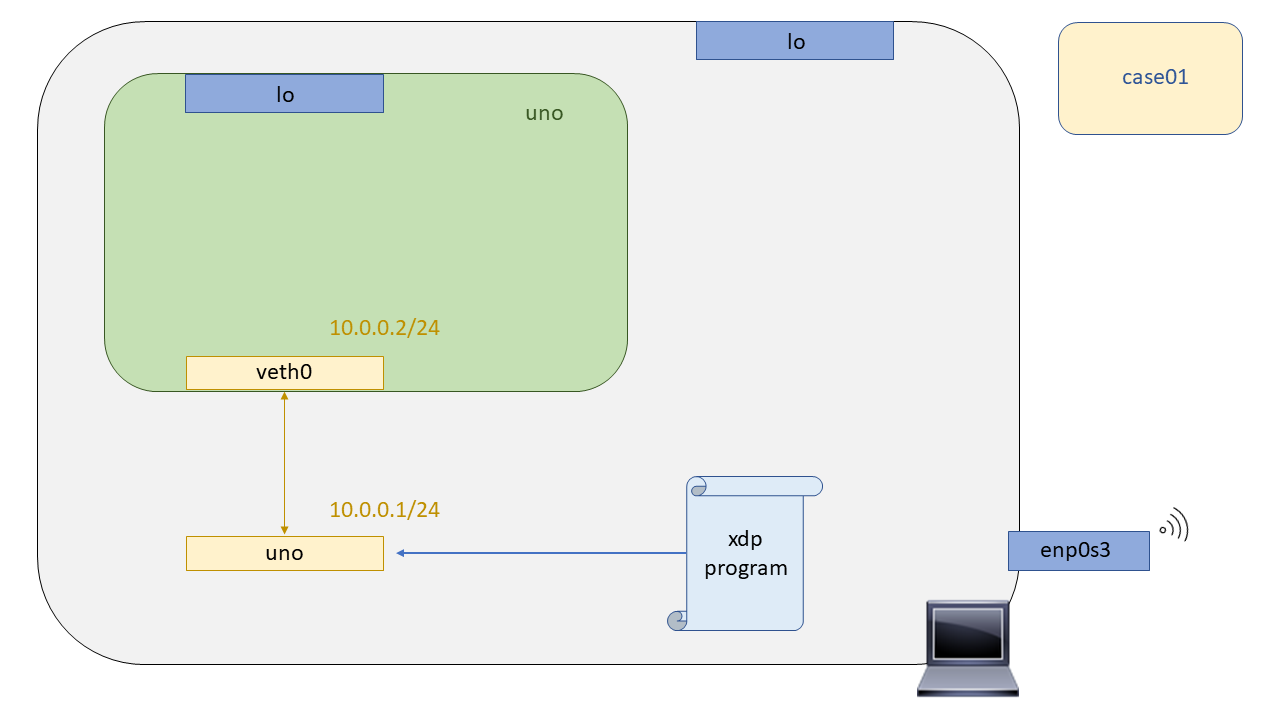
\includegraphics[width=16cm]{archivos/img/dev/xdp/case01/scenario.png}
    \caption{Escenario cableado del Case01 - XDP}
    \label{fig:case01_xdp_ether_scenario}
\end{figure}

\vspace{0.9cm}
\textbf{Carga del programa XDP}\\
\par

Es hora de cargar el programa \gls{xdp} en el Kernel. Para realizarlo, habría
dos maneras de cargar el bytecode en el Kernel. La primera sería hacer uso de la herramienta iproute2 (\ref{iproute2}) a partir de la versión \texttt{v4.12}. La segunda, y la más utilizada debido a las limitaciones de iproute2 para trabajar con los mapas \gls{bpf}, es hacer uso de la librería \textbf{libbpf}\footnote{\url{https://github.com/libbpf/libbpf}}. En este caso se hará uso de un programa hecho en C haciendo uso de dicha librería para cargar los programas \gls{xdp} en el kernel, mapas \gls{bpf} y demás. El código de dicho programa se puede encontrar \href{https://github.com/davidcawork/TFG/blob/master/src/use_cases/xdp/util/xdp_loader.c}{\textbf{aquí}}. Este \textit{loader} fue desarrollado siguiendo el tutorial de los desarrolladores del kernel de Linux llamado xdp-tutorial\footnote{\url{https://github.com/xdp-project/xdp-tutorial}}. \\
\par
Al \textit{loader} se le está indicando \texttt{-d} (\textit{device}), \texttt{-F} (\textit{Force}) para que haga un \textit{override} en caso de que ya haya un programa \gls{xdp} anclado a dicha interfaz, y por último, se le indica el \texttt{--progsec} (\textit{program section}) utilizados en \gls{xdp} para englobar distintas funcionalidades en un mismo \textit{bytecode} compilado. 

\begin{lstlisting}[language= bash, style=Consola, caption={Carga del programa XDP - Case01},label=code:case01_xdp_ether_load]
    # Cargaremos el programa sobre la interfaz "uno" 
    sudo ./xdp_loader -d uno -F --progsec xdp_case01
\end{lstlisting}

\vspace{1cm}
\textbf{Comprobación del funcionamiento}\\
\par

Una vez que el programa \gls{xdp} fue anclado a la interfaz se comprobará de que funciona según lo esperado. Esto se hará generando tráfico desde un extremo de una \gls{veth} para que atraviese por la interfaz que tiene anclado el programa \gls{xdp}. En este caso el comportamiento esperado del programa \gls{xdp} es que haga un drop de los paquetes nada más llegar a la interfaz \texttt{uno}.

% figura escenario
\begin{figure}[ht]
    \centering
    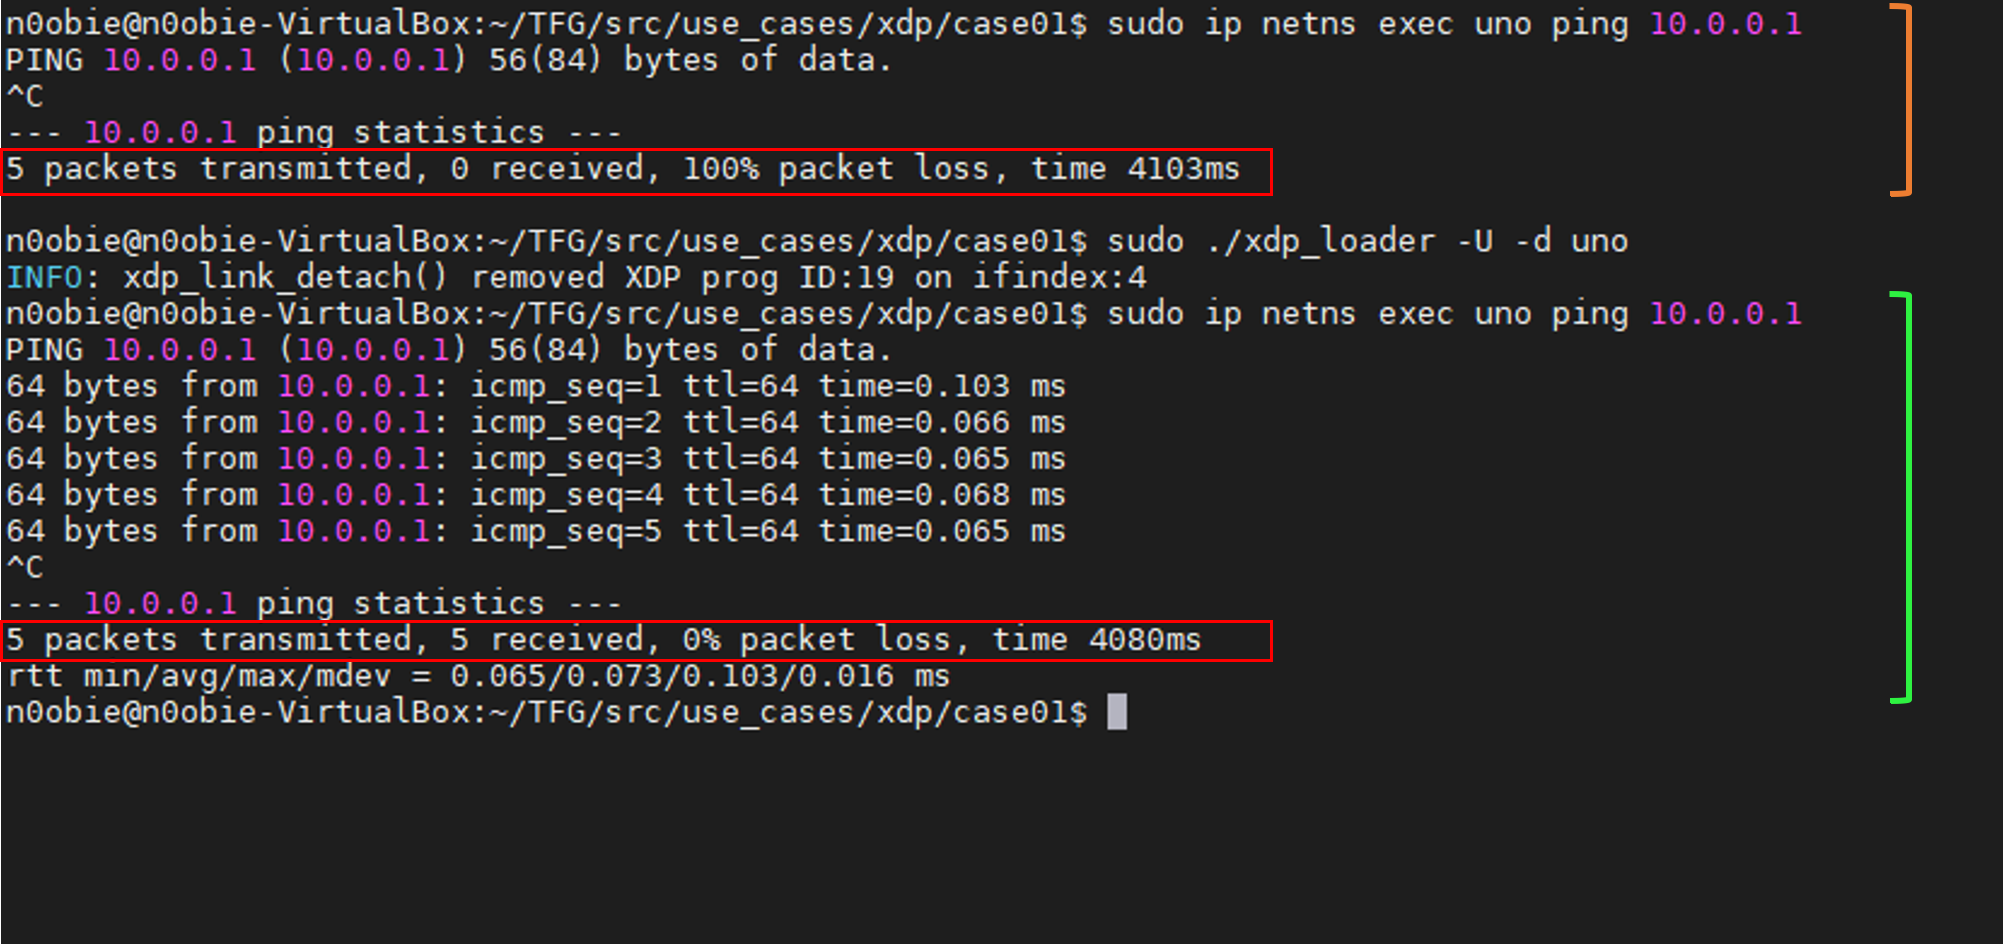
\includegraphics[width=15.5cm]{archivos/img/dev/xdp/case01/demo_case01_edited.png}
    \caption{Comprobación de funcionamiento del Case01 - XDP}
    \label{fig:case01_xdp_ether_func}
\end{figure}

Como se puede ver en la figura \ref{fig:case01_xdp_ether_func}, se accede al interior de la \textit{Network namespace} \texttt{uno} y se realiza un ping \fcolorbox{black}{orange}{\rule{0pt}{2.5pt}\rule{2.5pt}{0pt}}\hspace{1mm}  hacia la interfaz con el programa XDP. Se puede apreciar que no hay conectividad, por lo que el programa \gls{xdp} desarrollado está funcionando según lo esperado. Para corroborar que la falta de conectividad se debe al programa \gls{xdp}, se va a desanclar de la interfaz y se probará de nuevo la conectividad. Según se puede ver en el último ping \fcolorbox{black}{green}{\rule{0pt}{2.5pt}\rule{2.5pt}{0pt}} , ya hay conectividad, por lo que se afirma que realmente los paquetes que atravesaban la interfaz eran descartados por el programa \gls{xdp}. \newpage





\subsection{Case02 - Pass}
\label{xdp_ether_case02}

En este caso de uso se probará que es posible admitir todos los paquetes recibidos en la interfaz donde está anclado el programa \gls{xdp}. Pero podría surgir la siguiente pregunta: ¿qué significa ``Admitir”? Se quiere comprobar si es posible dejar pasar los paquetes, sin que les afecte el datapath programado con la tecnología. El motivo es que, aunque \gls{xdp} se concibe normalmente como como un mecanismo para hacer un \textit{by-pass} al \textit{stack} de red del Kernel de Linux (es decir, una completa redefinición del mismo), en muchas ocasiones será útil trabajar en conjunto para conseguir la funcionalidad deseada. \\
\par
Para la realizar la prueba, al igual que en el case01 (\ref{xdp_ether_case01}) primero se deberá compilar el programa \gls{xdp}, acto seguido levantar el escenario donde se va a realizar la prueba, y por último, anclar el binario a una interfaz del escenario.

\begin{lstlisting}[language=C, style=C-color, caption={Programa básico XDP - Case01},label=code:case02_xdp_ether_kernprog]
    SEC("xdp_case02")
    int xdp_pass_func(struct xdp_md *ctx)
    {
    	int action = XDP_PASS;
    	goto out;
    out:
            return xdp_stats_record_action(ctx, action);
    }
    
    char _license[ ] SEC("license") = "GPL";
\end{lstlisting}
\vspace{0.5cm}

Como se puede ver en el bloque \ref{code:case02_xdp_ether_kernprog}, el programa es exactamente igual al desarrollado en el case01 (\ref{xdp_ether_case01}) cambiando únicamente el código de retorno \gls{xdp}. De esta forma se consigue modificar la funcionalidad del programa, a la deseada.\\

\vspace{0.3cm}
\textbf{Compilación}\\
\par

Para compilar el programa \gls{xdp} se ha dejado un Makefile preparado en este directorio al igual que en el case01 (\ref{xdp_ether_case01}), por lo que para compilarlo únicamente hay que seguir las indicaciones del bloque \ref{code:case02_xdp_ether_compilacion}.

\begin{lstlisting}[language= bash, style=Consola, caption={Compilación programa XDP - Case02},label=code:case02_xdp_ether_compilacion]
    # En caso de no haber entrado en el directorio asignado del caso de uso
    cd TFG/src/use_cases/xdp/case02
    
    
    # Hacemos uso del Makefile suministrado 
    sudo make
\end{lstlisting}
\vspace{0.5cm}

Ahora bien, en el anterior caso de uso no se quiso incidir demasiado en este aspecto, pero ¿Cómo se produce la compilación de los programas \gls{xdp}?  Como ya se ha podido ver, los programas \gls{xdp} están escritos en lo que llaman un lenguaje C restringido, en los cuales la secuencia de programa siempre empieza por ``xdp". Esto es así ya que, si no, el verificador del Kernel no podrá saber de que tipo de \textit{bytecode} se trata y lo rechazará.\\
\par

Este código C restringido, se compilará haciendo uso de la herramienta \textbf{clang} cómo compilador de \textit{frontend}, y de la herramienta \textbf{LLVM} cómo compilador de  \textit{backend}. De esta manera se generará un \textit{bytecode} \gls{bpf}, y posteriormente se almacenará en un objeto de tipo \gls{elf}. Estos últimos serán los que se carguen en el Kernel (\texttt{*.o}). Es curioso el hecho de entender cómo pasamos de los hipotéticos programas \gls{xdp} (C restringido) a \textit{bytecode} \gls{bpf}, ya que, cuando se indaga un poco más en \gls{xdp}, se llega a la conclusión de que \gls{xdp} se podría ver como un \textit{framework} de \gls{bpf} para trabajar a nivel de \gls{nic}.\\
\par
Hay más factores que lo diferencian de los programas \gls{bpf}, como son las estructuras de datos que manejan, además de los metadatos; pero al fin y al cabo, para anclar un programa \gls{xdp} este debe antes ser traducido a un \textit{bytecode} \gls{bpf}.\\

\vspace{0.7cm}
\textbf{Puesta en marcha del escenario}\\
\par

Para testear los programas \gls{xdp} se hará uso de las \textit{Network Namespaces} (más información en la sección \ref{namespaces}). Como ya se comentaba, para que no suponga una barrera de entrada el concepto de las \textit{Network Namespaces}, se ha dejado escrito un script para levantar el escenario, y para su posterior limpieza. Es importante señalar que el script debe ser lanzado con permisos de root. Para levantar el escenario se debe ejecutar dicho script como se indica en el bloque \ref{code:case02_xdp_ether_escenario}.\\
\par
Para limpiar la máquina del escenario recreado anteriormente, se puede correr el mismo script indicándole ahora el parámetro \texttt{-c} (\textit{Clean}). En el peor de los casos, y si se cree que la limpieza se no se ha realizado de manera satisfactoria, se puede llevar a cabo un reinicio de la máquina consiguiendo así que todos los entes no persistentes (\gls{veth}, netns..) desaparezcan del equipo.

\begin{lstlisting}[language= bash, style=Consola, caption={Puesta en marcha del escenario - Case02},label=code:case02_xdp_ether_escenario]
    # Para levantar el escenario (Importante hacerlo con permisos de super usuario)
    sudo ./runenv.sh -i
    
    
    # Una vez finalizado la comprobación del caso de uso, limpiaremos nuestra maquina:
    sudo ./runenv.sh -c
\end{lstlisting}
\vspace{0.5cm}

El escenario que se va a manejar en este caso de uso es el siguiente (Ver figura \ref{fig:case02_xdp_ether_scenario}), compuesto únicamente de una \textit{Network Namespace} (\texttt{uno}) y un par de \gls{veth}s (\texttt{veth0} -- \texttt{uno}) para comunicar la \textit{Network Namespace} creada con la \textit{Network Namespace} por defecto.

\newpage

% figura escenario
\begin{figure}[ht]
    \centering
    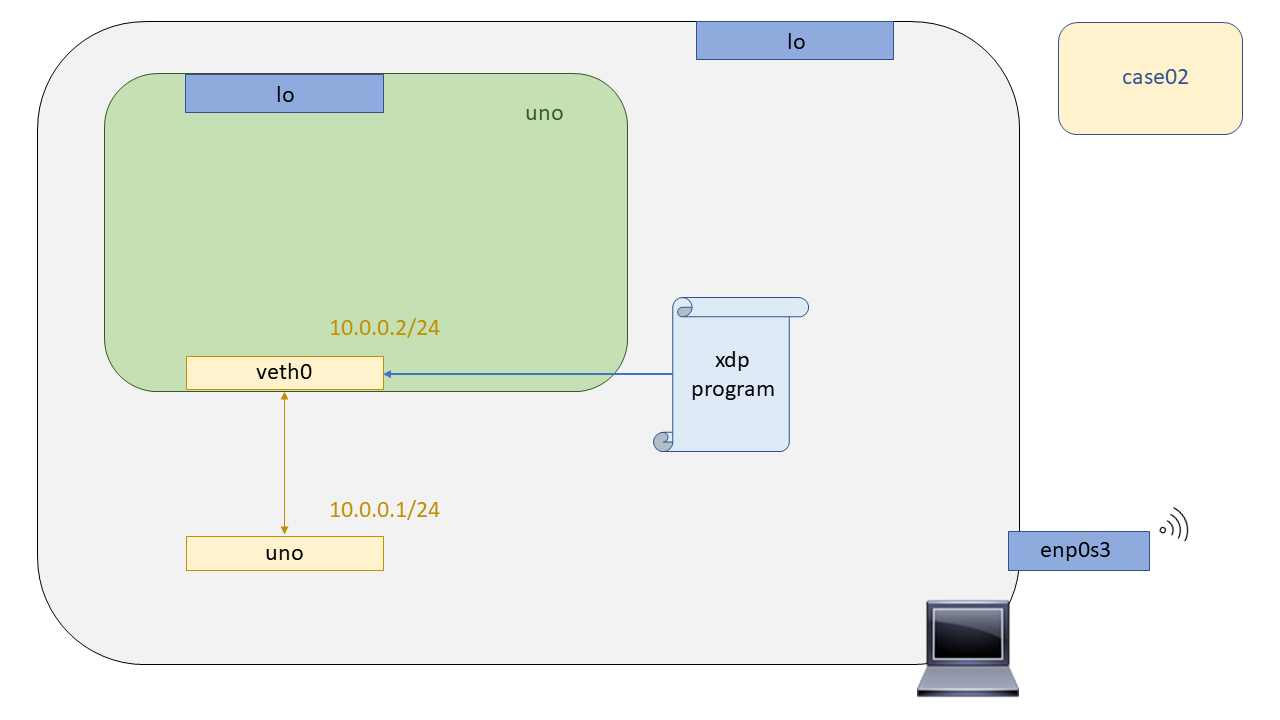
\includegraphics[width=16cm]{archivos/img/dev/xdp/case02/scenario.png}
    \caption{Escenario cableado del Case02 - XDP}
    \label{fig:case02_xdp_ether_scenario}
\end{figure}

\vspace{0.5cm}
\textbf{Carga del programa \gls{xdp}}\\
\par
Una vez que se tiene el escenario y el programa \gls{xdp} compilado, se procederá a cargarlo en el Kernel. Para más información sobre el programa  xdp\_loader, qué aporta la librería libbpf, o por que no se hace uso de la herramienta iproute2 para cargar los programas \gls{xdp} en el Kernel, se recomienda regresar al case01 (\ref{xdp_ether_case01})  donde se intenta abordar todas estas cuestiones.\\
\par

Como se comentaba, es hora de cargar el programa en el Kernel, esta vez por variar se va a cargar el programa \gls{xdp} en el extremo de la \gls{veth} que se encuentra en el interior de la \textit{Network Namespace}. Se podría haber hecho de la misma manera que en el caso de uso anterior y cargar el programa \gls{xdp} en la \gls{veth} que se ve desde la \textit{Network Namespace} por defecto, pero de esta manera se explorará como ejecutar comandos ``dentro" de una \textit{Network Namespace}. Para ejecutar comandos ``dentro" de una \textit{Network Namespace} se hará uso de la herramienta iproute2 (\ref{iproute2}), más concretamente su módulo llamado \textbf{netns}. A la herramienta se le debe indicar el parámetro \texttt{exec} y el nombre de la \textit{Network Namespace} dónde se quiera ejecutar el comando, y por último, se le indicará el comando que correrá ``dentro" de la \textit{Network Namespace}.

\begin{lstlisting}[language= bash, style=Consola, caption={Carga del programa XDP - Case02},label=code:case02_xdp_ether_load]
    # Cargaremos el programa sobre la interfaz "veth0" 
    sudo ip netns exec uno ./xdp_loader -d veth0 -F --progsec xdp_case02
\end{lstlisting}
\vspace{0.2cm}

Por lo que, entendiendo como funciona el módulo netns, y los parámetros suministrados al programa xdp\_loader, explicados en el caso de uso case01 (\ref{xdp_ether_case01}), se podrá intuir que el resultado de la sentencia anterior es la de cargar el programa \gls{xdp} en la interfaz llamada \texttt{veth0} contenida en la \textit{Network Namespace} \texttt{uno}.


\vspace{1.2cm}
\textbf{Comprobación del funcionamiento}\\
\par


La comprobación del funcionamiento del programa \gls{xdp} anclado a la interfaz \texttt{veth0} se llevará a cabo testeando la conectividad entre el par de \gls{veth}s. Puede que sea una prueba un poco simple, pero es suficiente, ya que únicamente se quiere verificar que el programa anclado en la interfaz está delegando los paquetes que le llegan, al \textit{stack} de red.\\
\par

En este punto se quiere comentar un aspecto de \gls{xdp}, y es que, desde que se empezó a trabajar con \gls{xdp}, se veía al \textit{stack} de red de Linux como a un enemigo a batir, o ``by-passear"; ya que con \gls{xdp} se quiere conseguir definir de manera exclusiva el datapath que se desea implementar con un equipo que porte el Kernel de Linux.  De esta manera, se consigue técnicamente un rendimiento superior ya que se quita de encima toda la redundancia y capas que no son necesarias para el procesamiento del hipotético datapath.\\
\par
Ahora bien, en el transcurso del aprendizaje con esta tecnología se ha visto que en ocasiones trabajar de manera cooperativa con el \textit{stack} de red puede reportar muchas facilidades y muchas otras funcionalidades ya implementadas en éste. No es cuestión de reinventar la rueda, más que nada porque el rendimiento que se puede llegar a ganar por hacer todo el procesamiento de manera exclusiva en la propia \gls{nic}, en opinión del autor, no compensa con la robustez y fiabilidad que tendrá dicha funcionalidad en el \textit{stack} de red de Linux.\\
\par
Como se puede apreciar en la figura \ref{fig:case02_xdp_ether_func}, prestando atención al ping \fcolorbox{black}{green}{\rule{0pt}{2.5pt}\rule{2.5pt}{0pt}}  (Fig. \ref{fig:case02_xdp_ether_func_ping}), hay perfecta conectividad. Eso significa que el programa \gls{xdp} está delegando correctamente los paquetes al \textit{stack} de red, se puede verificar dicho funcionamiento atendiendo a las estadísticas sobre los códigos de retorno de la figura \ref{fig:case02_xdp_ether_func_stats}, dónde el código de retorno \texttt{XDP\_PASS} va en aumento. Dichas estadísticas han sido recolectadas haciendo uso del binario xdp\_stats. En el siguiente caso de uso se explicará brevemente el funcionamiento de la recolección de estadísticas de los programas \gls{xdp}. 
\newpage

\begin{figure}[h!]
    \centering
    \begin{subfigure}[b]{\textwidth}
    	\centering
        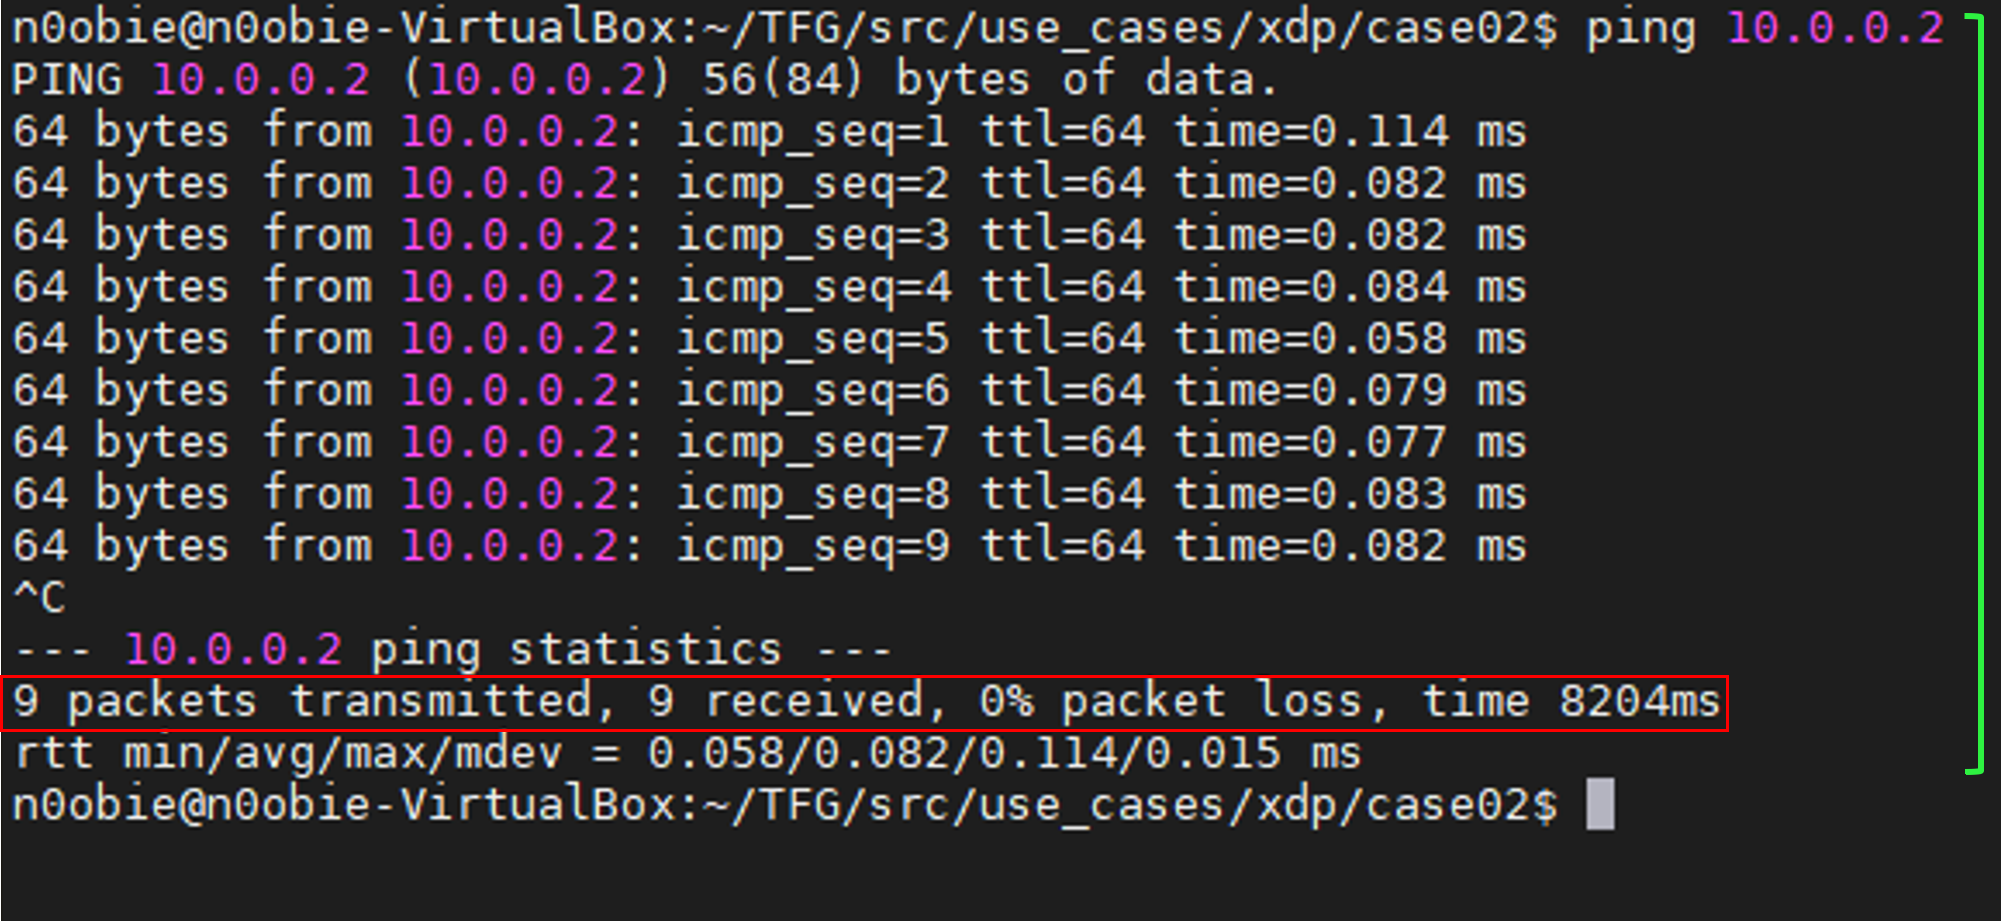
\includegraphics[width=11cm]{archivos/img/dev/xdp/case02/demo_case02_3_edited.png}
        \caption{Ejecución de ping hacia la interfaz con el programa XDP}
        \label{fig:case02_xdp_ether_func_ping}
    \end{subfigure}
    \par\bigskip
    \begin{subfigure}[b]{\textwidth}
    	\centering
    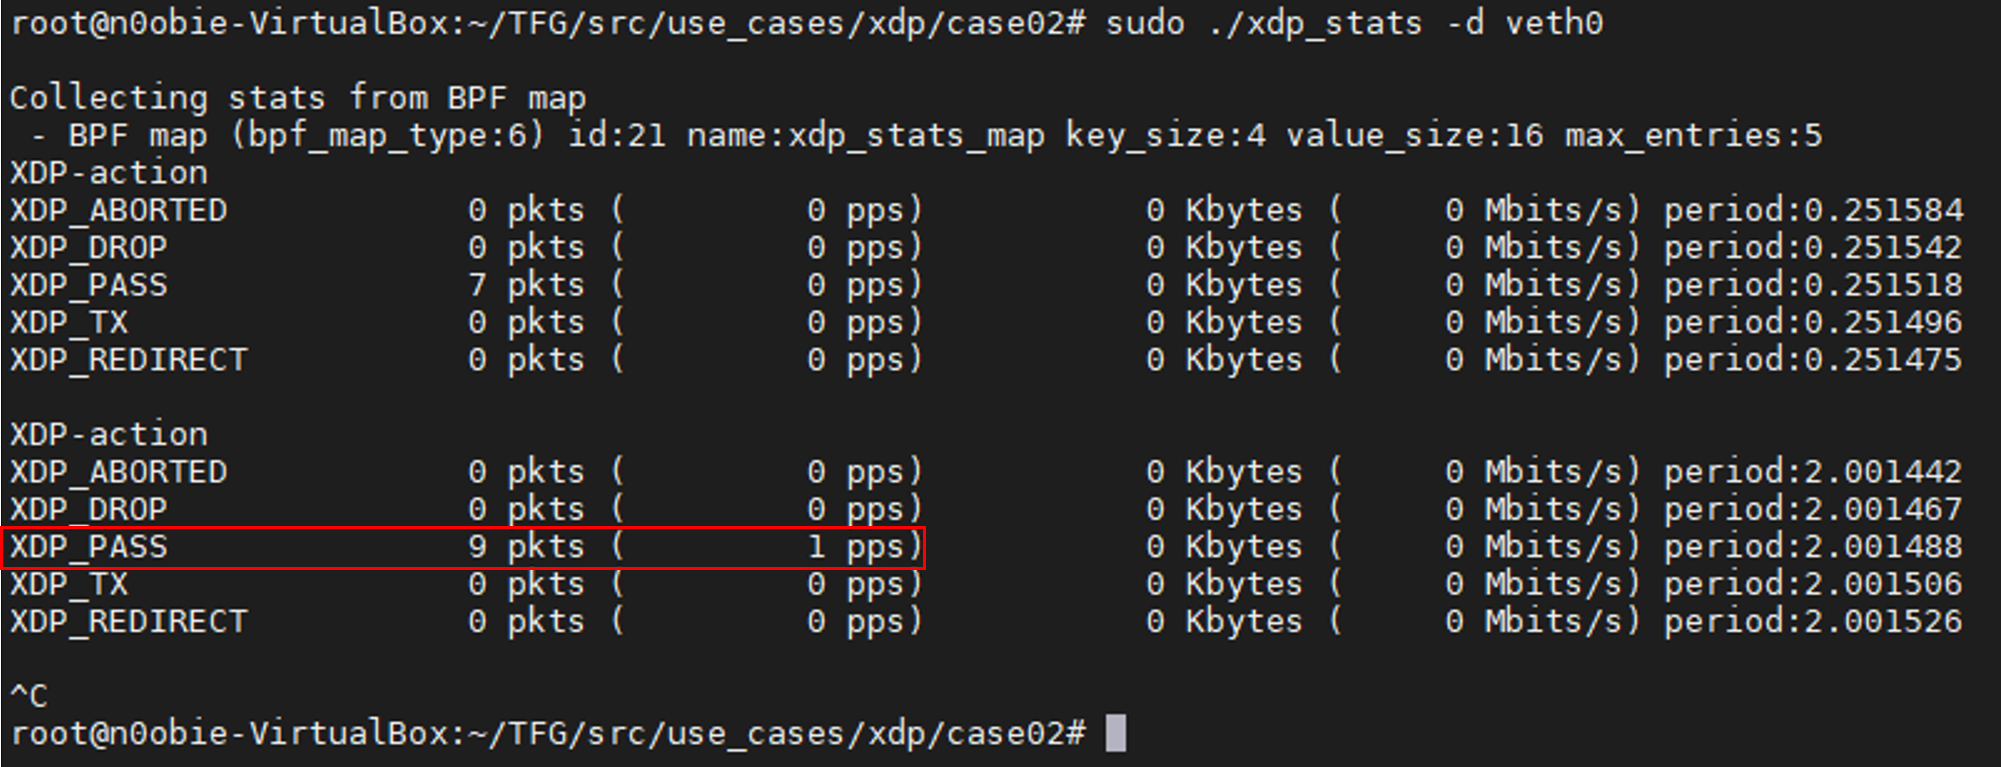
\includegraphics[width=14cm]{archivos/img/dev/xdp/case02/demo_case02_4_edited.png}
        \caption{Estadísticas de los códigos de retorno XDP}
        \label{fig:case02_xdp_ether_func_stats}
    \end{subfigure}
    \caption{Comprobación de funcionamiento del Case02 - XDP}
    \label{fig:case02_xdp_ether_func}
\end{figure}


\vspace{0.3cm}
\subsection{Case03 - Echo server}
\label{xdp_ether_case03}


En este caso de uso se hará un especial hincapié en el análisis de paquetes, su filtrado y manejo. En los anteriores caso de uso se definía un comportamiento de los paquetes haciendo un uso exclusivo de los códigos de retorno \gls{xdp}, más concretamente \texttt{XDP\_DROP} para tirar los paquetes y \texttt{XDP\_PASS} para admitir los paquetes. Hay más códigos de retorno \gls{xdp} pero con ellos no se puede lograr desarrollar todas las lógicas posibles. Como ya se comentaba en la sección \ref{TecnologiaXDP}, estos códigos se encuentran definidos en el archivo de cabecera \texttt{bpf.h}. En la tabla \ref{tab:xdp_return_code} se pueden recordar y ver qué funcionalidad aportaba cada uno de ellos.\\
\par
\vspace{0.3cm}

\begin{table}[ht]
\centering
\resizebox{\textwidth}{!}{%
\begin{tabular}{|c|c|}
\hline
\rowcolor[HTML]{EFEFEF} 
\multicolumn{1}{|l|}{\cellcolor[HTML]{EFEFEF}{\color[HTML]{24292E} \textbf{Código de Retorno}}} & \textbf{Comportamiento}                                                              \\ \hline
\texttt{XDP\_PASS}                                                                                       & Admitir el paquete, pasarselo al \textit{stack} de red                                        \\ \hline
\texttt{XDP\_DROP}                                                                                       & Tirar el paquete                                                                     \\ \hline
\texttt{XDP\_ABORTED}                                                                                    & Tirar el paquete y generar una \texttt{xdp:xdp\_exception}, útiles para depurar               \\ \hline
\texttt{XDP\_REDIRECT}                                                                                   & Utilizado cuando se realiza un forwarding del paquete a otra interfaz                \\ \hline
\texttt{XDP\_TX}                                                                                         & Re-transmitir el paquete por la misma interfaz por la cual se ha recibido el paquete \\ \hline
\end{tabular}}
\caption{Resumen sobre los códigos de retorno XDP}
\label{tab:xdp_return_code}
\end{table}


Ahora bien, ¿Cómo se puede implementar una lógica más avanzada? Esto se podrá conseguir filtrando los paquetes, y en base al tipo de paquete aplicar unas acciones u otras haciendo uso de los códigos de retorno \gls{xdp}. Para filtrar paquetes, se tendrá que hacer uso de las estructuras de datos de los protocolos de red definidas en el Kernel de Linux. Además de hacer numerosas comprobaciones de limites de acceso a memoria, para que el verificador del Kernel no nos tire el paquete por un acceso indebido según se comentaba en las limitaciones \gls{xdp} (Sección \ref{TecnologiaXDP}). Las estructuras de datos que han sido utilizadas para filtrar paquetes en este caso de uso se dejan indicadas en la tabla \ref{tab:xdp_structs}.\\
\par


\begin{table}[ht]
\centering

\begin{tabular}{|c|c|}
\hline
\rowcolor[HTML]{EFEFEF} 
\multicolumn{1}{|l|}{\cellcolor[HTML]{EFEFEF}{\color[HTML]{24292E} \textbf{Estructura}}} & \multicolumn{1}{l|}{\cellcolor[HTML]{EFEFEF}{\color[HTML]{24292E} \textbf{Archivo de cabecera}}} \\ \hline
\texttt{struct ethhdr}                                                                            & \texttt{<linux/if\_ether.h>}                                                                               \\ \hline
\texttt{struct ipv6hdr}                                                                           & \texttt{<linux/ipv6.h>}                                                                                   \\ \hline
\texttt{struct iphdr}                                                                             & \texttt{<linux/ip.h>}                                                                                     \\ \hline
\texttt{struct icmp6hdr}                                                                          & \texttt{<linux/icmpv6.h>}                                                                                 \\ \hline
\texttt{struct icmphdr}                                                                           & \texttt{<linux/icmp.h>}                                                                                   \\ \hline
\end{tabular}
\caption{Estructuras de datos para procesar las cabeceras de los paquetes}
\label{tab:xdp_structs}
\end{table}


Es importante señalar que los paquetes vienen por la red en un \textit{byte order} denominado como  \textit{Network byte order}. Por esta razón, se necesitará traducirlo al \textit{byte order} usado por la máquina ( \textit{Host order} ) en el caso de que se quiera comprobar o hacer uso del valor de algunos de sus campos. Para ello, se hará uso de las funciones \texttt{bpf\_ntohs()} y \texttt{bpf\_htons()} respectivamente.\\
\par

Por lo tanto, sabiendo qué estructuras de datos utilizar para el filtrando los paquetes, se filtrarán todos los paquetes de tipo ICMP - ICMPv6 con un código \texttt{ICMP-ECHO}. El resto de paquetes se le delegarán al \textit{stack} de red para que los maneje. En cuanto a los paquetes ICMP filtrados, se contestarán  automáticamente desde el programa \gls{xdp} desarrollado. Esto se conseguirá en la propia \gls{nic}, cambiando el \texttt{ICMP-ECHO} por un \texttt{ICMP-REPLY}, cambiando MACs, y por último, actualizando el \textit{checksum} de la cabecera ICMP. Como en este caso el paquete debe ser reenviado por la misma interfaz por la cual se recibió, se hará uso de código de retorno \texttt{XDP\_TX}.

\vspace{1cm}
\textbf{Compilación}\\
\par

Para compilar el programa \gls{xdp} se ha dejado un Makefile preparado en este directorio al igual que en el case02 (\ref{xdp_ether_case02}), por lo que para compilarlo únicamente hay que seguir las indicaciones del bloque \ref{code:case03_xdp_ether_compilacion}.

\begin{lstlisting}[language= bash, style=Consola, caption={Compilación programa XDP - Case03},label=code:case03_xdp_ether_compilacion]
    # En caso de no haber entrado en el directorio asignado del caso de uso
    cd TFG/src/use_cases/xdp/case03
    
    
    # Hacemos uso del Makefile suministrado 
    sudo make
\end{lstlisting}
\vspace{0.5cm}

Para más información sobre el proceso de compilación del programa \gls{xdp}, recomendamos que vuelva al case02 (\ref{xdp_ether_case02}) donde se hace referencia al flujo dispuesto para la compilación de los programas \gls{xdp}.


\vspace{0.7cm}
\textbf{Puesta en marcha del escenario}\\
\par
Para comprobar el funcionamiento de los programas \gls{xdp} se hará uso de nuevo de las \textit{Network Namespace} (más información en la sección \ref{namespaces}). Como ya se comentaba, para que no suponga una barrera de entrada el concepto de las \textit{Network Namespace}, se ha dejado escrito un script para levantar el escenario, y para su posterior limpieza. Es importante señalar que el script debe ser lanzado con permisos de root. Para levantar el escenario debemos ejecutar dicho script como se indica en el bloque \ref{code:case03_xdp_ether_escenario}. Para limpiar la máquina del escenario recreado anteriormente, se puede correr el mismo script indicándole ahora el parámetro \texttt{-c} (\textit{Clean}). En el peor de los casos, y si se cree que la limpieza se no se ha realizado de manera satisfactoria, se puede llevar a cabo un reinicio de la máquina consiguiendo así que todos los entes no persistentes (\gls{veth}, netns..) desaparezcan del equipo.

\begin{lstlisting}[language= bash, style=Consola, caption={Puesta en marcha del escenario - Case03},label=code:case03_xdp_ether_escenario]
    # Para levantar el escenario (Importante hacerlo con permisos de super usuario)
    sudo ./runenv.sh -i
    
    
    # Una vez finalizado la comprobación del caso de uso, limpiaremos nuestra máquina:
    sudo ./runenv.sh -c
\end{lstlisting}
\vspace{0.5cm}

El escenario que se va a manejar en este caso de uso es el siguiente (Ver figura \ref{fig:case03_xdp_ether_scenario}), compuesto únicamente de una \textit{Network Namespace} (\texttt{uno}) y un par de \gls{veth}s (\texttt{veth0} -- \texttt{uno}) para comunicar la \textit{Network Namespace} creada con la \textit{Network Namespace} por defecto.

% figura escenario
\begin{figure}[ht]
    \centering
    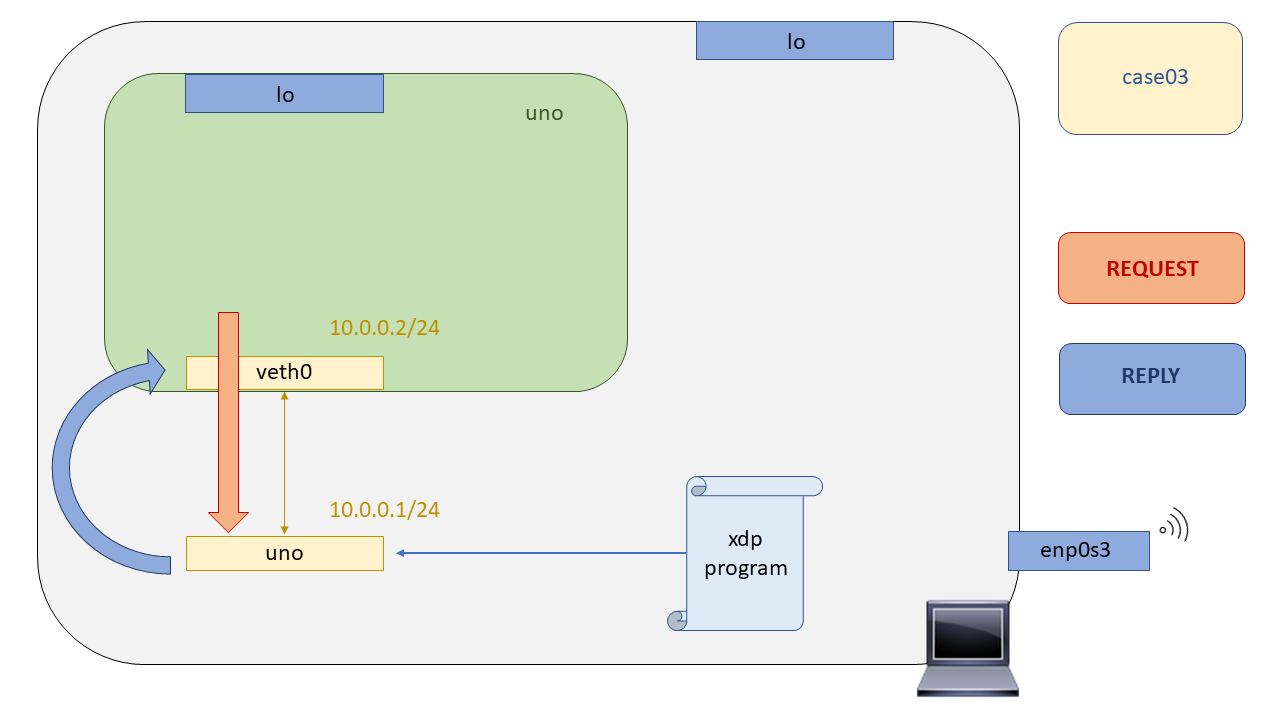
\includegraphics[width=16cm]{archivos/img/dev/xdp/case03/scenario.png}
    \caption{Escenario cableado del Case03 - XDP}
    \label{fig:case03_xdp_ether_scenario}
\end{figure}


\vspace{0.7cm}
\textbf{Carga del programa XDP}\\
\par
Una vez que se tiene el escenario levantado y el programa \gls{xdp} compilado, se procederá a cargarlo en el Kernel. Para más información sobre el programa xdp\_loader, qué aporta la librería libbpf, o por que no se hace uso de la herramienta iproute2 para cargar los programas \gls{xdp} en el Kernel,  se recomienda regresar al case01 (\ref{xdp_ether_case01})  donde se intenta abordar todas estas cuestiones. De forma adicional, es interesante comentar que se va hacer uso del módulo \textbf{netns} de la herramienta iproute2, si tiene alguna duda sobre dicho módulo le recomendamos que consulte su \textit{man-page} o vuelva al case02 (\ref{xdp_ether_case02}) donde se hace una pequeña introducción sobre éste, y su funcionamiento básico para ejecutar comandos ``dentro" de una \textit{Network Namespace}.

\begin{lstlisting}[language= bash, style=Consola, caption={Carga del programa XDP - Case03},label=code:case03_xdp_ether_load]
    # Anclamos el programa XDP (xdp_pass) en la interfaz veth0, perteneciente a la Network Namespace "uno" 
    sudo ip netns exec uno ./xdp_loader -d veth0 -F --progsec xdp_pass
    
    # Anclamos el programa XDP en la interfaz uno, perteneciente a la Network Namespace por defecto
    sudo ./xdp_loader -d uno -F --progsec xdp_case03
\end{lstlisting}
\vspace{0.5cm}

En este caso de uso se anclará el programa \gls{xdp} a validar en la \gls{veth} exterior, por lo que las pruebas vendrán inducidas desde ``dentro" de la \textit{Network Namespace} \texttt{uno}. Para anclar el programa se ha hecho uso de nuevo del programa xdp\_loader. Es importante señalar que se ha tenido que anclar un \textit{dummy program} que permite pasar todos los paquetes a la \gls{veth} destino, esta es una limitación propia por trabajar con \gls{veth}s y \gls{xdp}, de momento se trata de una limitación de implementación, pero puede que a un corto plazo esta limitación se vea ya superada. \\
\par
Para más información sobre esta limitación recomendamos ver la charla de la Netdev llamada ``\textit{\gls{veth}: \gls{xdp} for containers}"\footnote{\url{https://netdevconf.info/0x13/session.html?talk-veth-xdp}} donde explican con un mayor detalle la misma, cómo abordarla y por qué está inducida.

\vspace{0.5cm}
\textbf{Comprobación del funcionamiento}\\
\par

La comprobación del funcionamiento del programa \gls{xdp} anclado a la interfaz \texttt{uno} se llevará a cabo generando pings desde ``dentro" la \textit{Network Namespace} \texttt{uno} hacia afuera. De esta forma la interfaz \texttt{uno} los filtrará, analizará y generará una respuesta. \\
\par
El funcionamiento del programa xdp\_stats es muy simple, ya que desde el programa anclado en el Kernel se genera un mapa \gls{bpf} del tipo clave-valor, donde las claves son los distintos códigos de retorno y los valores son contadores. Después, desde el espacio de usuario el programa xdp\_stats, sabiendo el nombre del mapa \gls{bpf}, y dónde se almacena, va a buscarlo. Para ello, abre el descriptor de archivo asociado a ese mapa almacenado en el path \texttt{/sys/fs/bpf/}. Una vez que tiene abierto el descriptor de archivo, este irá leyendo por clave del mapa todas las estadísticas sobre los códigos de retorno de forma periódica.


\begin{figure}[ht]
    \centering
    \begin{subfigure}[b]{\textwidth}
    	\centering
        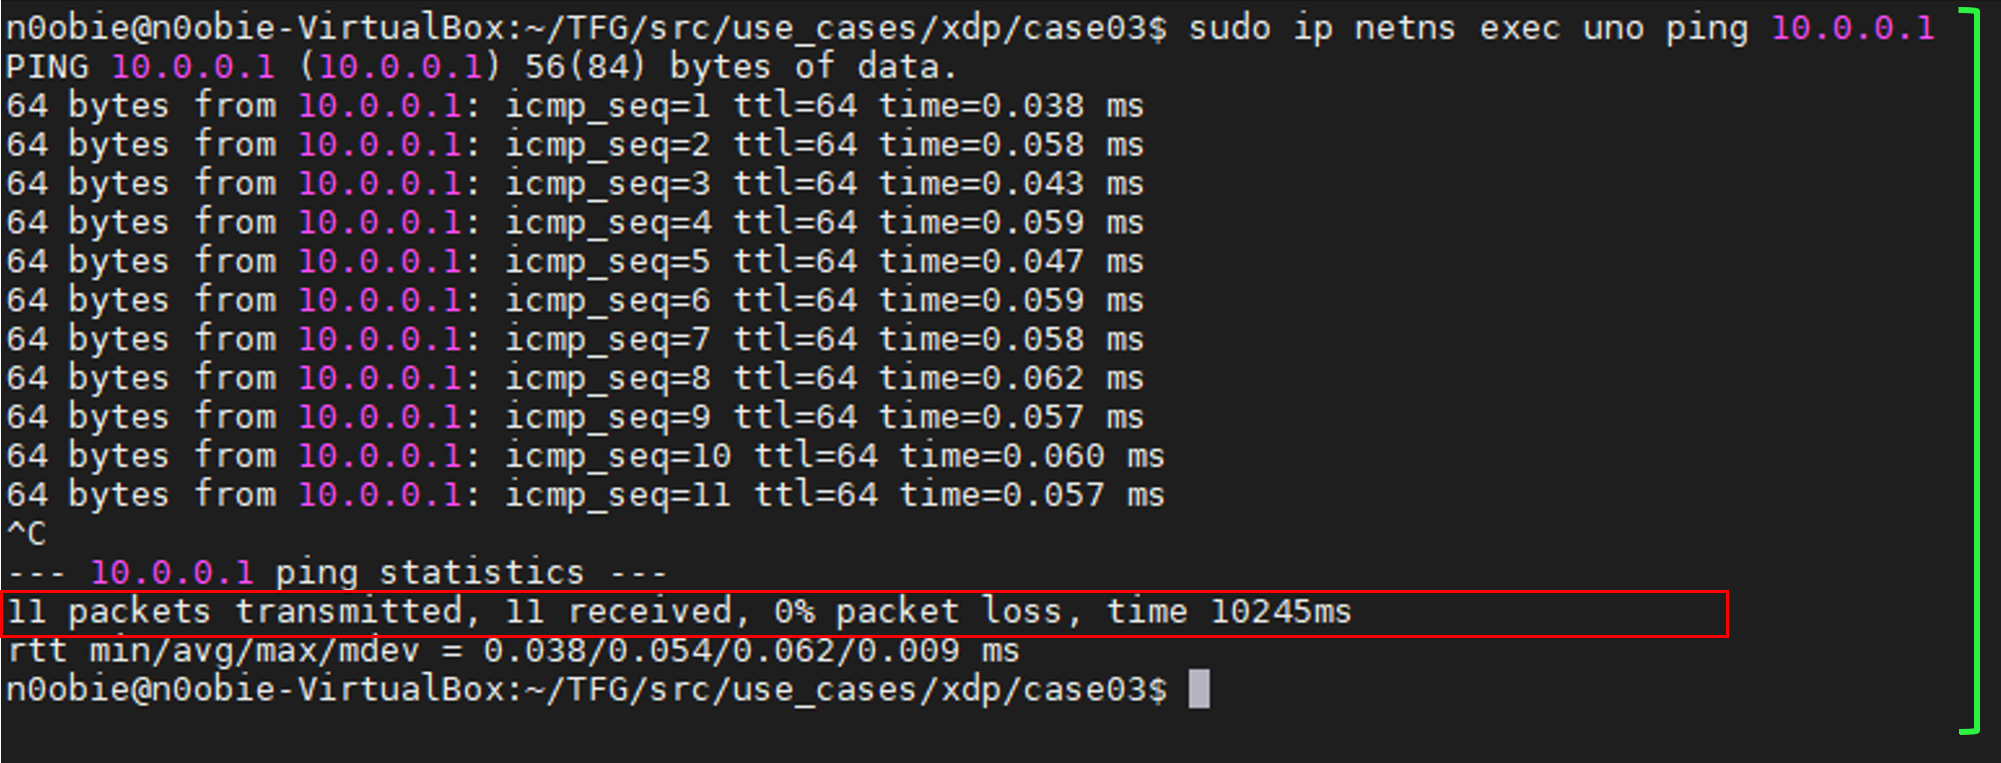
\includegraphics[width=12cm]{archivos/img/dev/xdp/case03/demo_case03_2_edited.png}
        \caption{Ejecución de ping hacia la interfaz con el programa XDP}
        \label{fig:case03_xdp_ether_func_ping}
    \end{subfigure}
    \par\bigskip
    \begin{subfigure}[b]{\textwidth}
    	\centering
        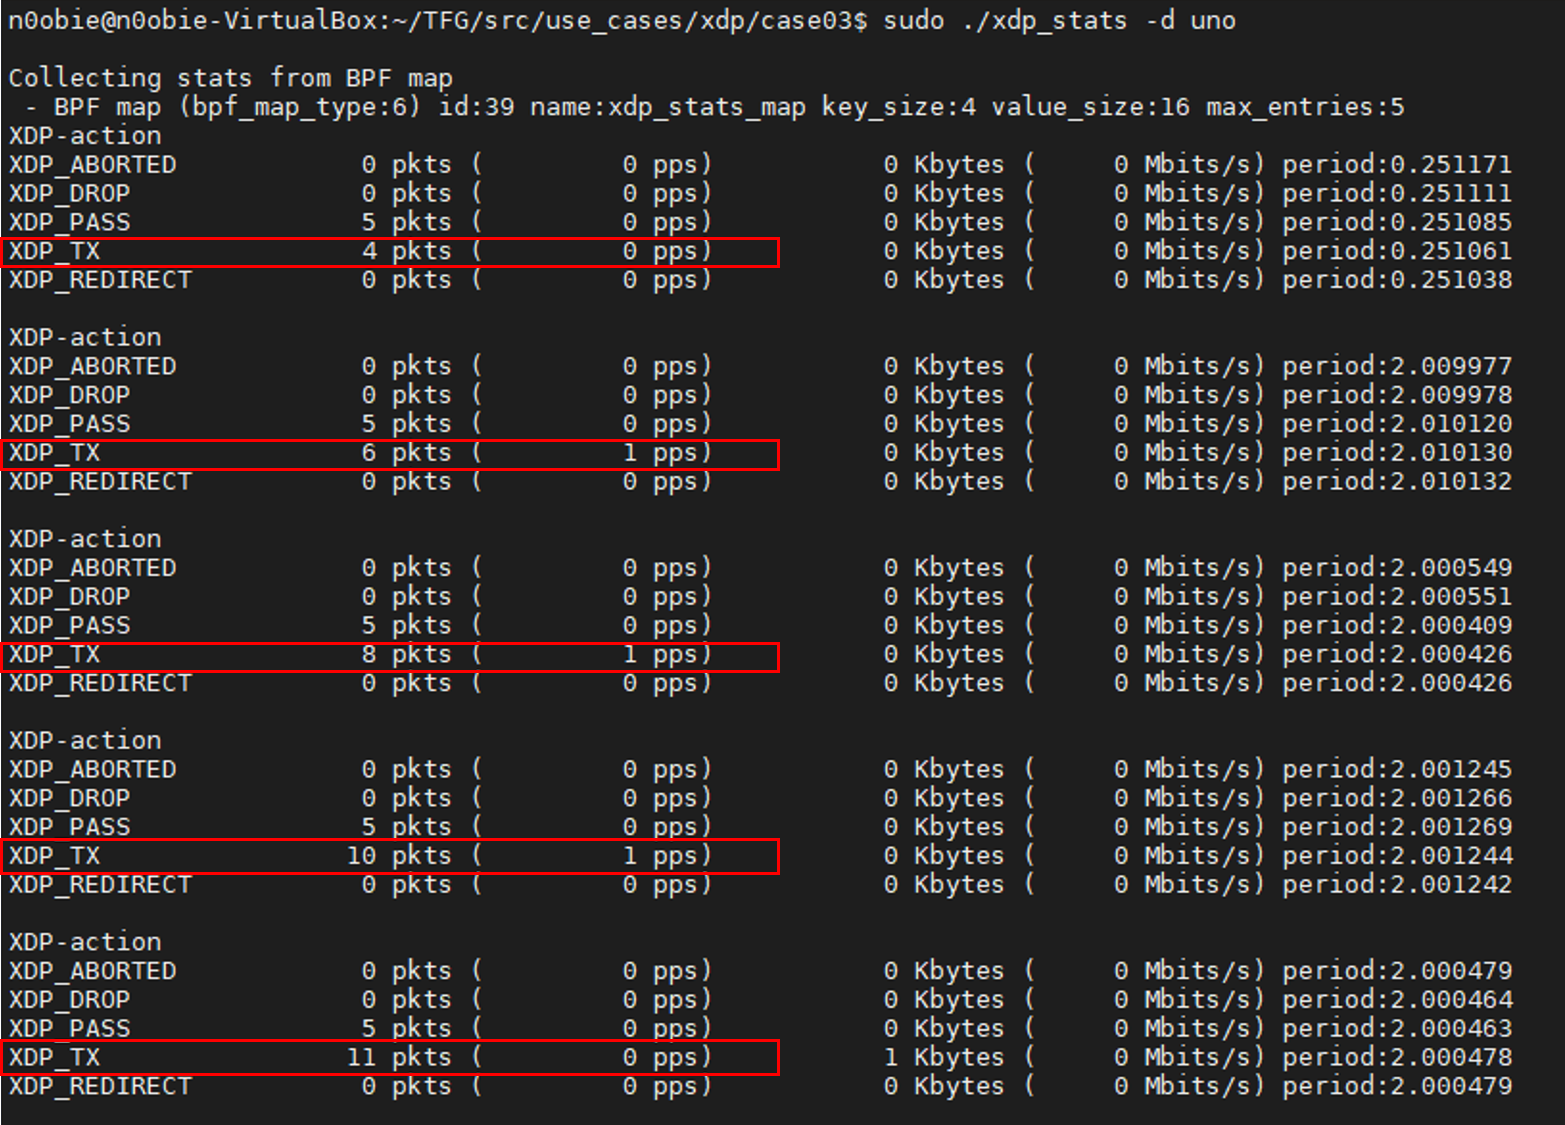
\includegraphics[width=11cm]{archivos/img/dev/xdp/case03/demo_case03_3_edited.png}
        \caption{Estadísticas de los códigos de retorno XDP}
        \label{fig:case03_xdp_ether_func_stats}
    \end{subfigure}
    \caption{Comprobación de funcionamiento del Case03 - XDP}
    \label{fig:case03_xdp_ether_func1}
\end{figure}

Si todo funciona correctamente se debería ver como los códigos de retorno mayormente empleados son los de \texttt{XDP\_TX} siempre y cuando no se haya detenido el ping  desde dentro de la \textit{Network Namespace}. Como se puede apreciar en la figura \ref{fig:case03_xdp_ether_func1}, el ping \fcolorbox{black}{green}{\rule{0pt}{2.5pt}\rule{2.5pt}{0pt}}\hspace{1mm} está siendo contestado correctamente por el programa \gls{xdp} dado que los códigos \texttt{XDP\_TX} van aumentando.\\
\par
De forma adicional, se va a comprobar cómo todos los pings que se manden desde dentro de la \textit{Network Namespace} \texttt{uno} serán contestados. Esto es así, ya que el programa \gls{xdp}, contestará todos los \texttt{ECHO-REQUEST} que le lleguen independientemente de si van dirigidos a él. En la figura \ref{fig:case03_xdp_ether_func2} se puede ver cómo funciona un ping \fcolorbox{black}{orange}{\rule{0pt}{2.5pt}\rule{2.5pt}{0pt}}\hspace{1mm} a una máquina inexistente. Para ello, se ha tenido que añadir una MAC inventada en la tabla ARP asociada a la IP a la cual vamos hacer ping  para que no se iniciara una resolución ARP. En el caso de que se iniciara una resolución ARP, el ping estaría bloqueado a la espera de completar una resolución ARP sobre una máquina inexistente. 

\begin{figure}[h]
    \centering
    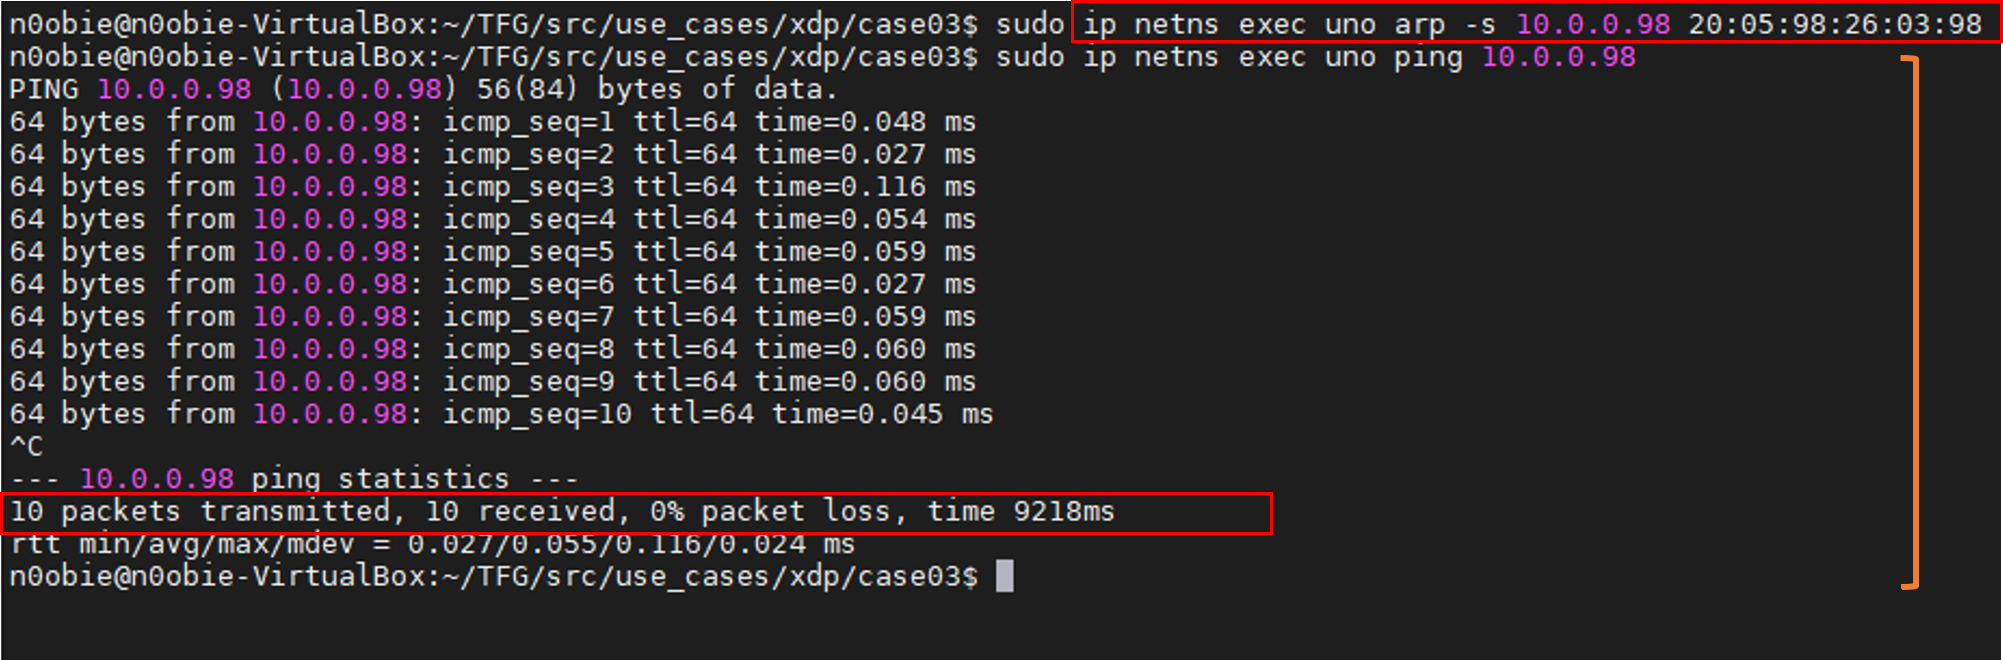
\includegraphics[width=14cm]{archivos/img/dev/xdp/case03/demo_case03_4_edited.png}
    \caption{Ping a máquina inexistente - XDP}
    \label{fig:case03_xdp_ether_func2}
\end{figure}

\subsection{Case04 - Layer 3 forwarding}
\label{xdp_ether_case04}

En este caso de uso se explorará como realizar forwarding de paquetes. En este punto, ya se ha revisado cómo filtrar por las cabeceras de los paquetes, analizarlos y establecer una lógica asociada a ese filtrado con los códigos de retorno \gls{xdp}. Una acción adicional a realizar con los paquetes será el forwarding. En \gls{xdp} vendrá implementado por códigos de retorno y por \textit{helpers} \gls{bpf} porque, como ya comentábamos en el case02 (\ref{xdp_ether_case02}), \gls{xdp} se termina traduciendo en \gls{bpf} (e\gls{bpf}), por lo que ciertas funciones, no todas, para trabajar con \gls{bpf} están disponibles a la hora de trabajar con \gls{xdp}.\\
\par

A lo largo de este caso de uso, se han explorado las distintas maneras para lograr el forwarding con \gls{xdp}. Se ha ido desde la manera más simple a la manera más robusta y, a su vez, compleja. Para que no haya diferencias entre las distintas formas de realizar el forwarding, se ha creado un mismo escenario donde se explorarán estas vías sin que existan diferencias inducidas por este. En el caso de uso anterior ya se estaba haciendo un forwarding, ya que, con el código \texttt{XDP\_TX} se realiza un forwarding hacia la interfaz por la cual se recibió dicho paquete. Pero, ¿cómo se hace un forwarding hacia otras interfaces? Leyendo la \textit{man-page} de los \textit{helpers} \gls{bpf} se han encontrado las funciones \texttt{bpf\_redirect()}, \texttt{bpf\_redirect\_map()}, las cuales, leyendo su descripción, serán la vía utilizada para abordar esta necesidad.

\begin{lstlisting}[language=C, style=C-color, caption={Helper BPF para realizar Forwarding - Case04},label=code:case04_xdp_ether_kernprog1]
    int bpf_redirect(u32 ifindex, u64 flags);

    int bpf_redirect_map(struct bpf_map *map, u32 key, u64 flags);
\end{lstlisting}


\vspace{0.5cm}
\textbf{Compilación}\\
\par

Para compilar el programa \gls{xdp} se ha dejado un Makefile preparado en este directorio al igual que en el case03 (\ref{xdp_ether_case03}), por lo que para compilarlo únicamente hay que seguir las indicaciones del bloque \ref{code:case04_xdp_ether_compilacion}.

\begin{lstlisting}[language= bash, style=Consola, caption={Compilación programa XDP - Case04},label=code:case04_xdp_ether_compilacion]
    # En caso de no haber entrado en el directorio asignado del caso de uso
    cd TFG/src/use_cases/xdp/case04
    
    # Hacemos uso del Makefile suministrado 
    sudo make
\end{lstlisting}
\vspace{0.5cm}

Podrá encontrar más información sobre el proceso de compilación de los programas \gls{xdp} en el case02 (\ref{xdp_ether_case02}).


\vspace{0.7cm}
\textbf{Puesta en marcha del escenario}\\
\par
Para comprobar el funcionamiento de los programas \gls{xdp} se hará uso de las \textit{Network Namespace} (más información en la sección \ref{namespaces}). Como ya se comentaba, para que no suponga una barrera de entrada el concepto de las \textit{Network Namespace}, se ha dejado escrito un script para levantar el escenario, y para su posterior limpieza. Es importante señalar que el script debe ser lanzado con permisos de root. Para levantar el escenario debemos ejecutar dicho script como se indica en el bloque \ref{code:case03_xdp_ether_escenario}. Para limpiar la máquina del escenario recreado anteriormente, se puede correr el mismo script indicándole ahora el parámetro \texttt{-c} (\textit{Clean}). En el peor de los casos, y si se cree que la limpieza se no se ha realizado de manera satisfactoria, se puede llevar a cabo un reinicio de la máquina consiguiendo así que todos los entes no persistentes (\gls{veth}, netns..) desaparezcan del equipo.

\begin{lstlisting}[language= bash, style=Consola, caption={Puesta en marcha del escenario - Case04},label=code:case04_xdp_ether_escenario]
    # Para levantar el escenario (Importante hacerlo con permisos de super usuario)
    sudo ./runenv.sh -i
    
    
    # Una vez finalizado la comprobación del caso de uso, limpiaremos nuestra maquina:
    sudo ./runenv.sh -c
\end{lstlisting}
\vspace{0.5cm}

%%%%%%%%%%%%%%%%%%%%%%%%%%%%%%%%%%%%%%%%%%%%%%%%%%%%%%%%%%%%%%%%%%%%%%%%%%%%%%%%%%%%

\subsubsection{Hardcoded forwarding}
\label{xdp_ether_case04_hard}

La primera forma de implementación del forwarding es lo que denominaremos como Hardcoded forwarding, dado que es necesario hardcodear\footnote{Hardcodear: perder flexibilidad y/o prolijidad dejando valores y/o comportamientos fijos en el código del programa.} información de forwarding en el propio programa \gls{xdp}. El escenario levantado se puede apreciar en la figura \ref{fig:case04_xdp_ether_scenario1}, está compuesto de dos \textit{Network Namespace} (\texttt{uno} y \texttt{dos}), y de dos pares de \gls{veth}s (\texttt{veth0} -- \texttt{uno} y \texttt{veth0} -- \texttt{dos}) las cuales se utilizarán para comunicar las dos \textit{Network Namespaces} entre sí, a través del la \textit{Network Namespace} por defecto. En este caso el forwarding lo haremos desde la interfaz \texttt{dos} hacia la interfaz \texttt{uno}.


% figura escenario
\begin{figure}[ht]
    \centering
    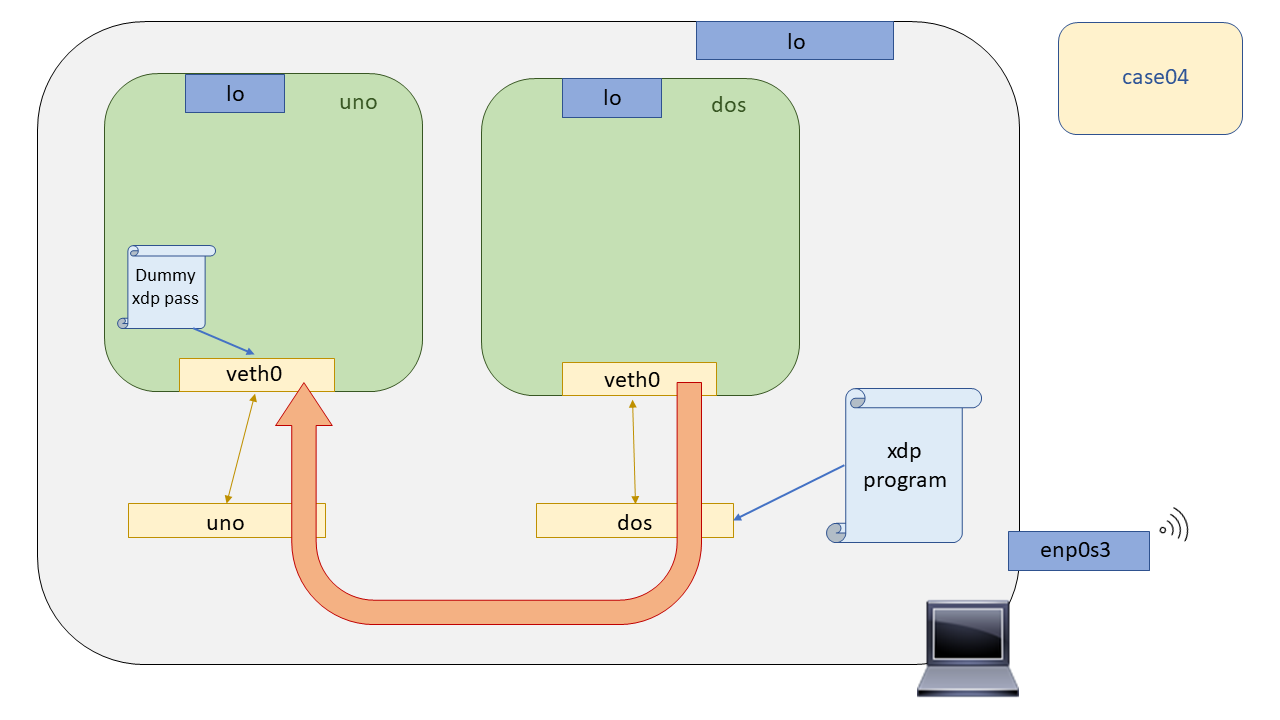
\includegraphics[width=16cm]{archivos/img/dev/xdp/case04/scenario_01.png}
    \caption{Escenario cableado Hardcoded forwarding del Case04 - XDP}
    \label{fig:case04_xdp_ether_scenario1}
\end{figure}


\vspace{0.5cm}
\textbf{Carga del programa XDP}\\
\par

Antes de realizar la carga del programa se deben obtener \textbf{dos datos}, la \textit{ifindex} de la interfaz uno a la cual se van a mandar los paquetes generados desde el interior de la \textit{Network Namespace} \texttt{dos}, y la MAC de la interfaz interna de la \textit{Network Namespace} \texttt{uno}, ya que será necesario que los paquetes que se dirijan a la interfaz \texttt{uno} lleven como MAC destino la de la \texttt{veth0}, para que así los paquetes no sean descartados.\\
\par
Una vez se tengan estos datos anotados se abrirá el programa \gls{xdp} (\texttt{*.c}) con cualquier editor de texto, se irá a la declaración de variables y se hardcodeará como se puede ver en el bloque \ref{code:case04_xdp_ether_kernprog2} tanto el \textit{ifindex} como la MAC.
\par

\begin{lstlisting}[language=C, style=C-color, caption={Ejemplo MAC e Ifindex - Case04},label=code:case04_xdp_ether_kernprog2]
    /*  Para un ifindex: 6 y una MAC: 9A:DE:AF:EC:18:6E */

    ...
    
    unsigned char dst[ETH_ALEN + 1] = {0x9a,0xde,0xaf,0xec,0x18,0x6e, '\0'} ;
    unsigned ifindex = 6; 

    ...
\end{lstlisting}
\vspace{0.5cm}
Una vez que se tenga hardcodeado los datos para realizar el forwarding se debe recompilar el programa \gls{xdp} para que el \textit{bytecode} que se ancle a la interfaz dos haga correctamente el forwarding. Por ello, simplemente se tiene que hacer un \textit{make} nuevamente.\\
\par
Por lo tanto, teniendo todo preparado es hora de anclar de nuevo el programa \gls{xdp}. Recordemos que por el estar trabajando con interfaz \gls{veth}s se debe anclar un \textit{dummy program}\footnote{\url{https://netdevconf.info/0x13/session.html?talk-veth-xdp}} en el extremo donde se vayan a recibir los paquetes.
\begin{lstlisting}[language= bash, style=Consola, caption={Carga del programa XDP Hardcoded forwarding - Case04},label=code:case04_xdp_ether_load1]
    # Entramos a la Network Namespace "uno" y anclamos el dummy program a la interfaz veth0
    sudo ip netns exec uno ./xdp_loader -d veth0 -F --progsec xdp_pass
    
    # Acto seguido, anclamos el programa a la interfaz "dos" como ya comentábamos antes
    sudo ./xdp_loader -d dos -F --progsec xdp_case04
\end{lstlisting}

\vspace{0.5cm}
\textbf{Comprobación del funcionamiento}\\
\par
La comprobación de funcionamiento de este programa \gls{xdp} es bastante básica, se va a generar paquetes desde el interior de la \textit{Network Namespace}  \texttt{dos} hacia la \gls{veth} interna de la \textit{Network Namespace} \texttt{uno}. Si todo funciona correctamente deberían llegar los paquetes en el sentido dispuesto del forwarding hardcodeado, sería una comunicación unidireccional. Para ello se abrirán tres terminales, en cada una de ellas se llevará a cabo una tarea. Ver bloque \ref{code:case04_xdp_ether_func1}, donde se indican todos los comandos necesarios para comprobar el funcionamiento del Hardcoded forwarding.

\begin{lstlisting}[language= bash, style=Consola, caption={Comprobación del funcionamiento Hardcoded forwarding - Case04},label=code:case04_xdp_ether_func1]
    # En esta terminal generaremos el ping hacia la interfaz de la Network Namespace "uno" desde la Network Namespace "dos"
    [Terminal:1] sudo ip netns exec dos ping {IP_veth0_uno}
    
    # En esta terminal pondremos a un sniffer a escuchar los paquetes que nos lleguen dentro de la Network Namespace "dos"
    [Terminal:2] sudo ip netns exec uno tcpdump -l
    
    # Por último, opcionalmente, podemos ejecutar el programa que actuaba como recolector de estadísticas sobre los códigos de retorno XDP
    [Terminal:3] sudo ./xdp_stats -d dos
\end{lstlisting}

% figura escenario
\begin{figure}[ht]
    \centering
    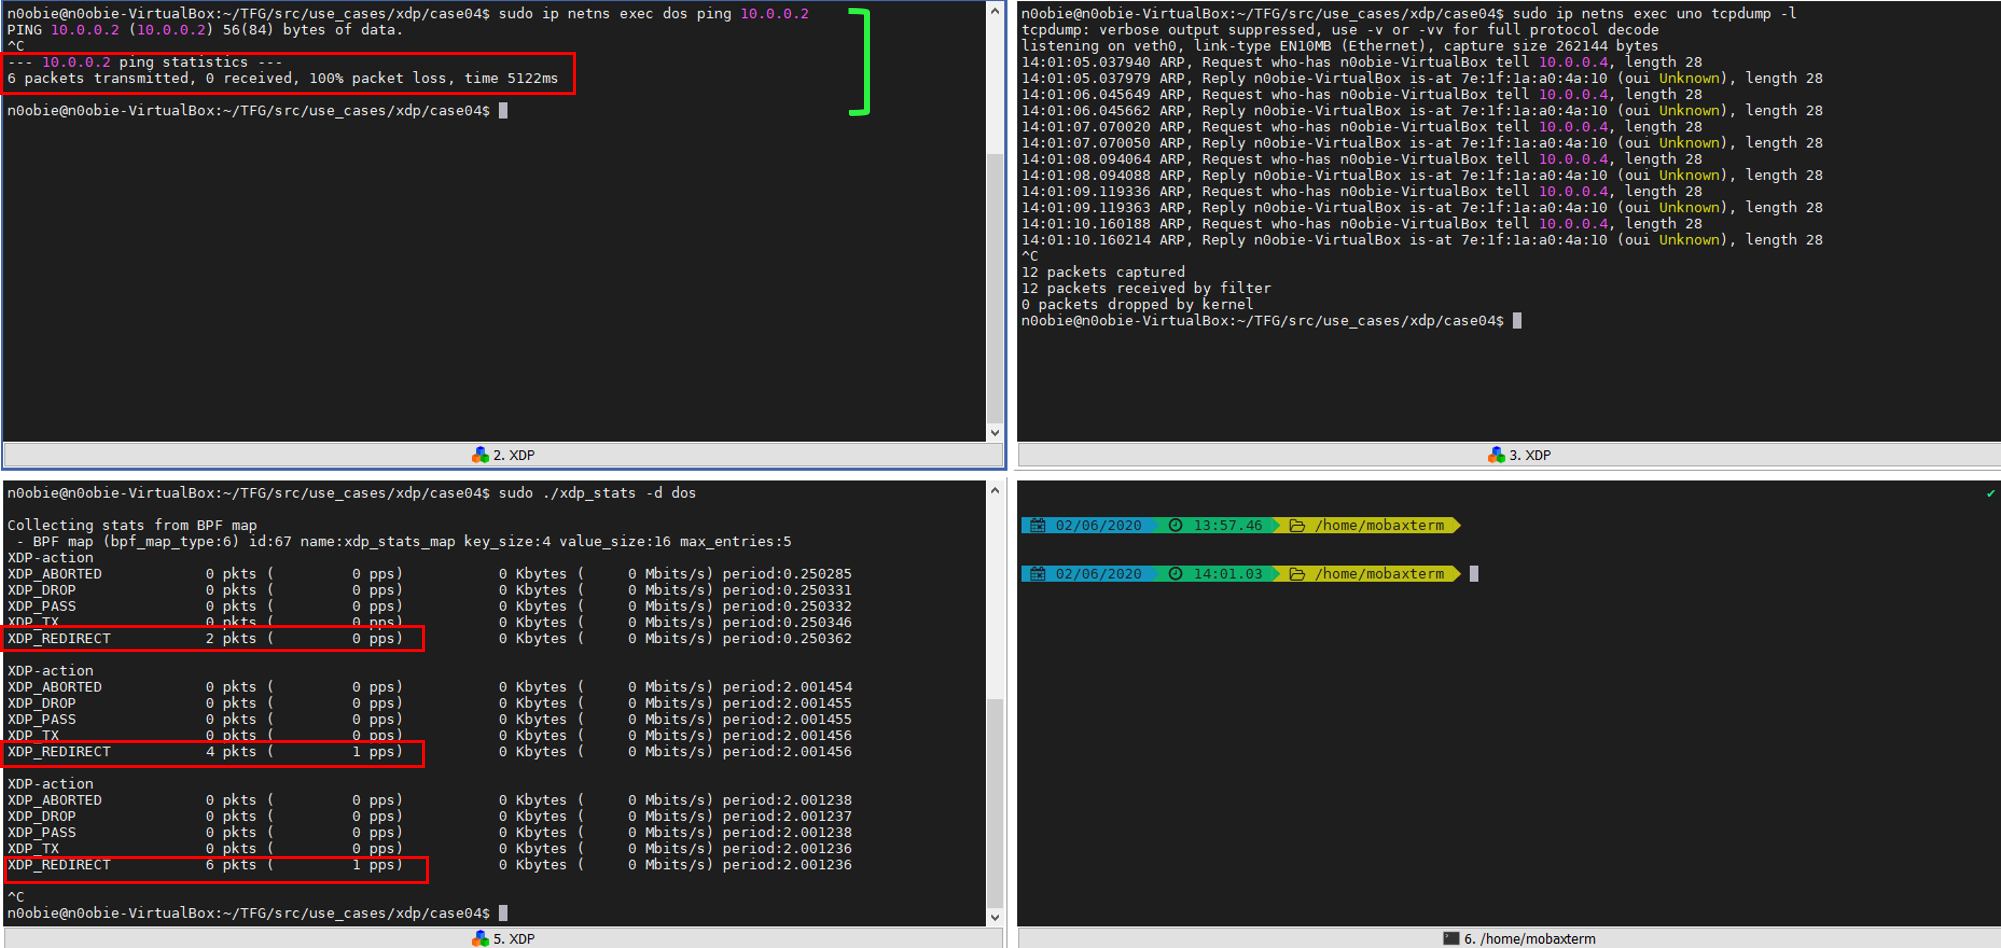
\includegraphics[width=15.5cm]{archivos/img/dev/xdp/case04/demo_case04_hard_1_edited.png}
    \caption{Comprobación de funcionamiento Hardcoded forwarding del Case04 - XDP}
    \label{fig:case04_xdp_ether_func1_b}
\end{figure}

Como se puede apreciar en la figura \ref{fig:case04_xdp_ether_func1_b}, el ping \fcolorbox{black}{green}{\rule{0pt}{2.5pt}\rule{2.5pt}{0pt}}\hspace{1mm} no llega a completarse. Esto se debe a que al implementar una comunicación unidireccional, el ping se queda bloqueado en la resolución ARP. Se puede corroborar este funcionamiento atendiendo a los códigos de retorno \gls{xdp}, \texttt{XDP\_REDIRECT}, como van en aumento debido a los reenvíos de los paquetes ARP-Request de una interfaz a la otra y por la escucha de tcpdump en la terminal superior derecha. 
%%%%%%%%%%%%%%%%%%%%%%%%%%%%%%%%%%%%%%%%%%%%%%%%%%%%%%%%%%%%%%%%%%%%%%%%%%%%%%%%%%%%

\subsubsection{Semi-Hardcoded forwarding (BPF maps)}

La segunda forma de implementar el forwarding se denominará Semi-Hardcoded forwarding, ya que la información irá hardcodeada, pero no en el propio programa \gls{xdp}, sino, en los mapas \gls{bpf}. El escenario levantado se puede apreciar en la figura \ref{fig:case04_xdp_ether_scenario2}, está compuesto de dos \textit{Network Namespace} (\texttt{uno} y \texttt{dos}), y de dos pares de \gls{veth}s (\texttt{veth0} -- \texttt{uno} y \texttt{veth0} -- \texttt{dos}) las cuales se utilizarán para comunicar las dos \textit{Network Namespaces} entre sí, a través del la \textit{Network Namespace} por defecto. En este caso el forwarding se hará desde la interfaz \texttt{dos} hacia la interfaz \texttt{uno} y viceversa, por lo que la comunicación será bidireccional.

% figura escenario
\begin{figure}[ht]
    \centering
    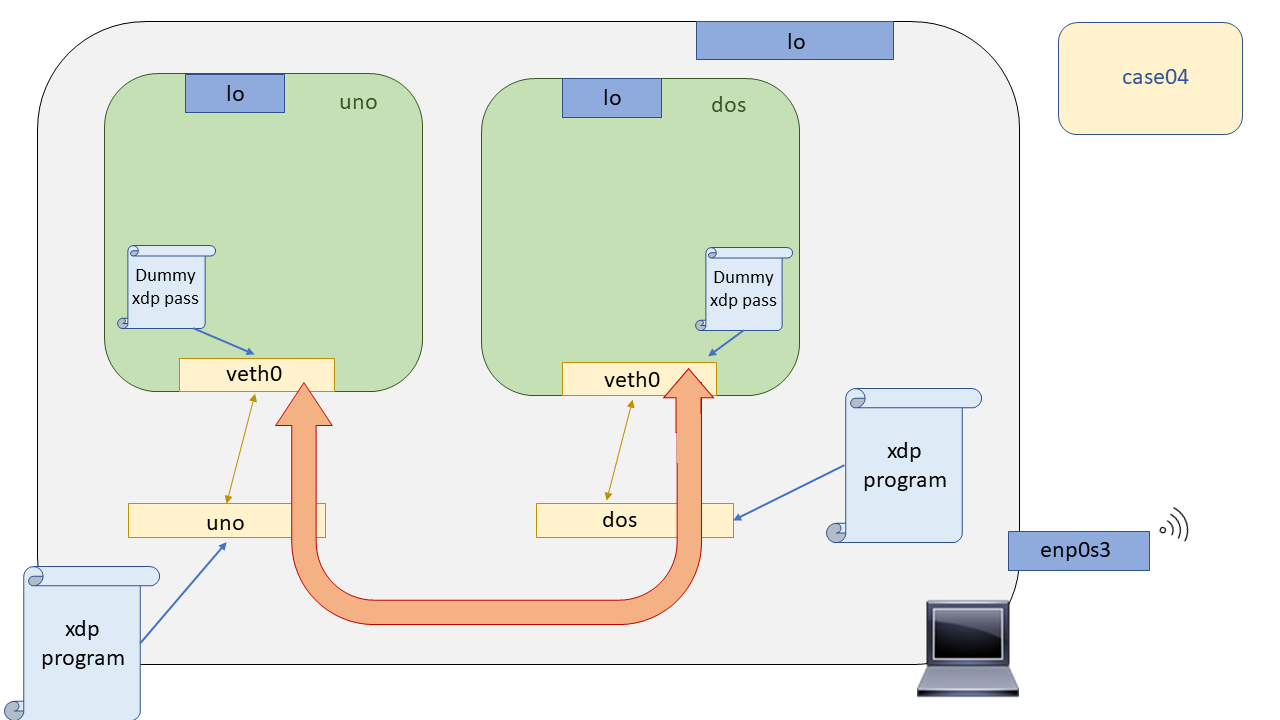
\includegraphics[width=14cm]{archivos/img/dev/xdp/case04/scenario_02.png}
    \caption{Escenario cableado Semi-Hardcoded forwarding del Case04 - XDP}
    \label{fig:case04_xdp_ether_scenario2}
\end{figure}

\vspace{1cm}
\textbf{Carga del programa XDP}\\
\par
Esta manera de hacer el forwarding no requiere de hardcodear datos en el propio programa \gls{xdp} que irá al Kernel, si no, que se usarán los mapas \gls{bpf} como medio para guardar datos de forwarding como son las \textit{ifindex} y las MAC destino desde espacio de usuario. De esta forma, posteriormente el programa anclado en el Kernel sea capaz de leer los mapas, obtener la información de forwarding y realizarlo en base a la información percibida de los mapas \gls{bpf}.\\
\par

De nuevo, y como en este caso la comunicación será bidireccional se debe anclar dos \textit{dummy program} en los dos extremos donde van a llegar los paquetes, si no se está al tanto de esta limitación vuelva a la subsección (\ref{xdp_ether_case04_hard}) donde se menciona la limitación.\\
\par

Es importante señalar que los programas anclados previamente deben ser retirados, por lo que una opción sería hacer un \textit{clean} del escenario haciendo uso del script dado ( \texttt{sudo ./runenv.sh -c}) y empezar de nuevo.\\
\par
\begin{lstlisting}[language= bash, style=Consola, caption={Carga del programa XDP Semi-Hardcoded forwarding - Case04},label=code:case04_xdp_ether_load2]
    # Entramos en cada Network Namespace y anclamos los "dummy programs"
    sudo ip netns exec uno ./xdp_loader -d veth0 -F --progsec xdp_pass
    sudo ip netns exec dos ./xdp_loader -d veth0 -F --progsec xdp_pass
    
    # Anclamos el programa XDP en cada interfaz para conseguir un comunicación bidireccional 
    sudo ./xdp_loader -d uno -F --progsec xdp_case04_map
    sudo ./xdp_loader -d dos -F --progsec xdp_case04_map
    
    # Almacenamos la información necesaria para realizar el forwarding 
    src="uno"
    dest="dos"
    src_mac=$(sudo ip netns exec $src cat /sys/class/net/veth0/address)
    dest_mac=$(sudo ip netns exec $dest cat /sys/class/net/veth0/address)
     
    # Populamos los mapas BPF con la información útil para llevar a cabo el forwarding en ambas direcciones
    ./prog_user -d $src -r $dest --src-mac $src_mac --dest-mac $dest_mac
    ./prog_user -d $dest -r $src --src-mac $dest_mac --dest-mac $src_mac
\end{lstlisting}


\vspace{1cm}
\textbf{Comprobación del funcionamiento}\\
\par
La comprobación de funcionamiento de este programa puede ser llevada a cabo desde un extremo u otro debido a que, si todo funciona correctamente, existirá una comunicación bidireccional. Por lo que, en este caso se harán las pruebas desde la \textit{Network namespace} \texttt{uno} hacia la \texttt{dos}.\\
\par
Como se puede apreciar en la figura \ref{fig:case04_xdp_ether_func2}, existe una comunicación bidireccional ya que el ping \fcolorbox{black}{orange}{\rule{0pt}{2.5pt}\rule{2.5pt}{0pt}}\hspace{1mm} se ejecuta con normalidad. Además, en la subfigura \ref{fig:case04_xdp_ether_func2_stats} se puede ver como los códigos de retorno \gls{xdp} de forwarding van aumentando, por lo que el programa \gls{xdp} está funcionando según lo previsto.

\begin{figure}[h]
    \centering
    \begin{subfigure}[b]{\textwidth}
    	\centering
        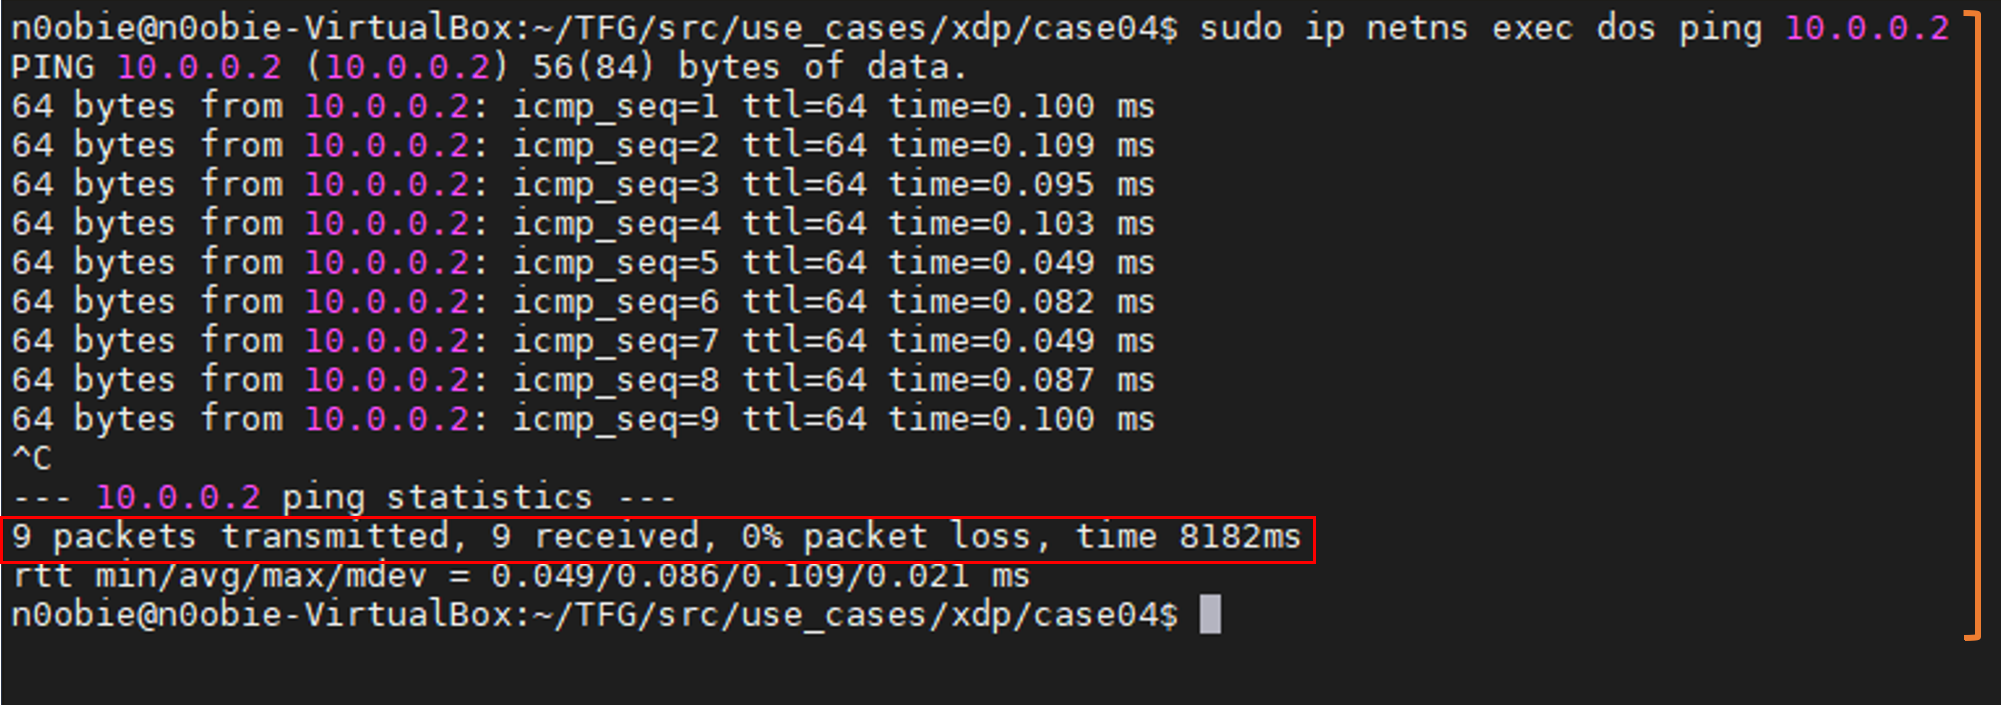
\includegraphics[width=11cm]{archivos/img/dev/xdp/case04/demo_case04_semihard_2_edited.png}
        \caption{Ejecución de ping hacia la interfaz con el programa XDP}
        \label{fig:case04_xdp_ether_func2_ping}
    \end{subfigure}
    \par\bigskip
    \begin{subfigure}[b]{\textwidth}
    	\centering
        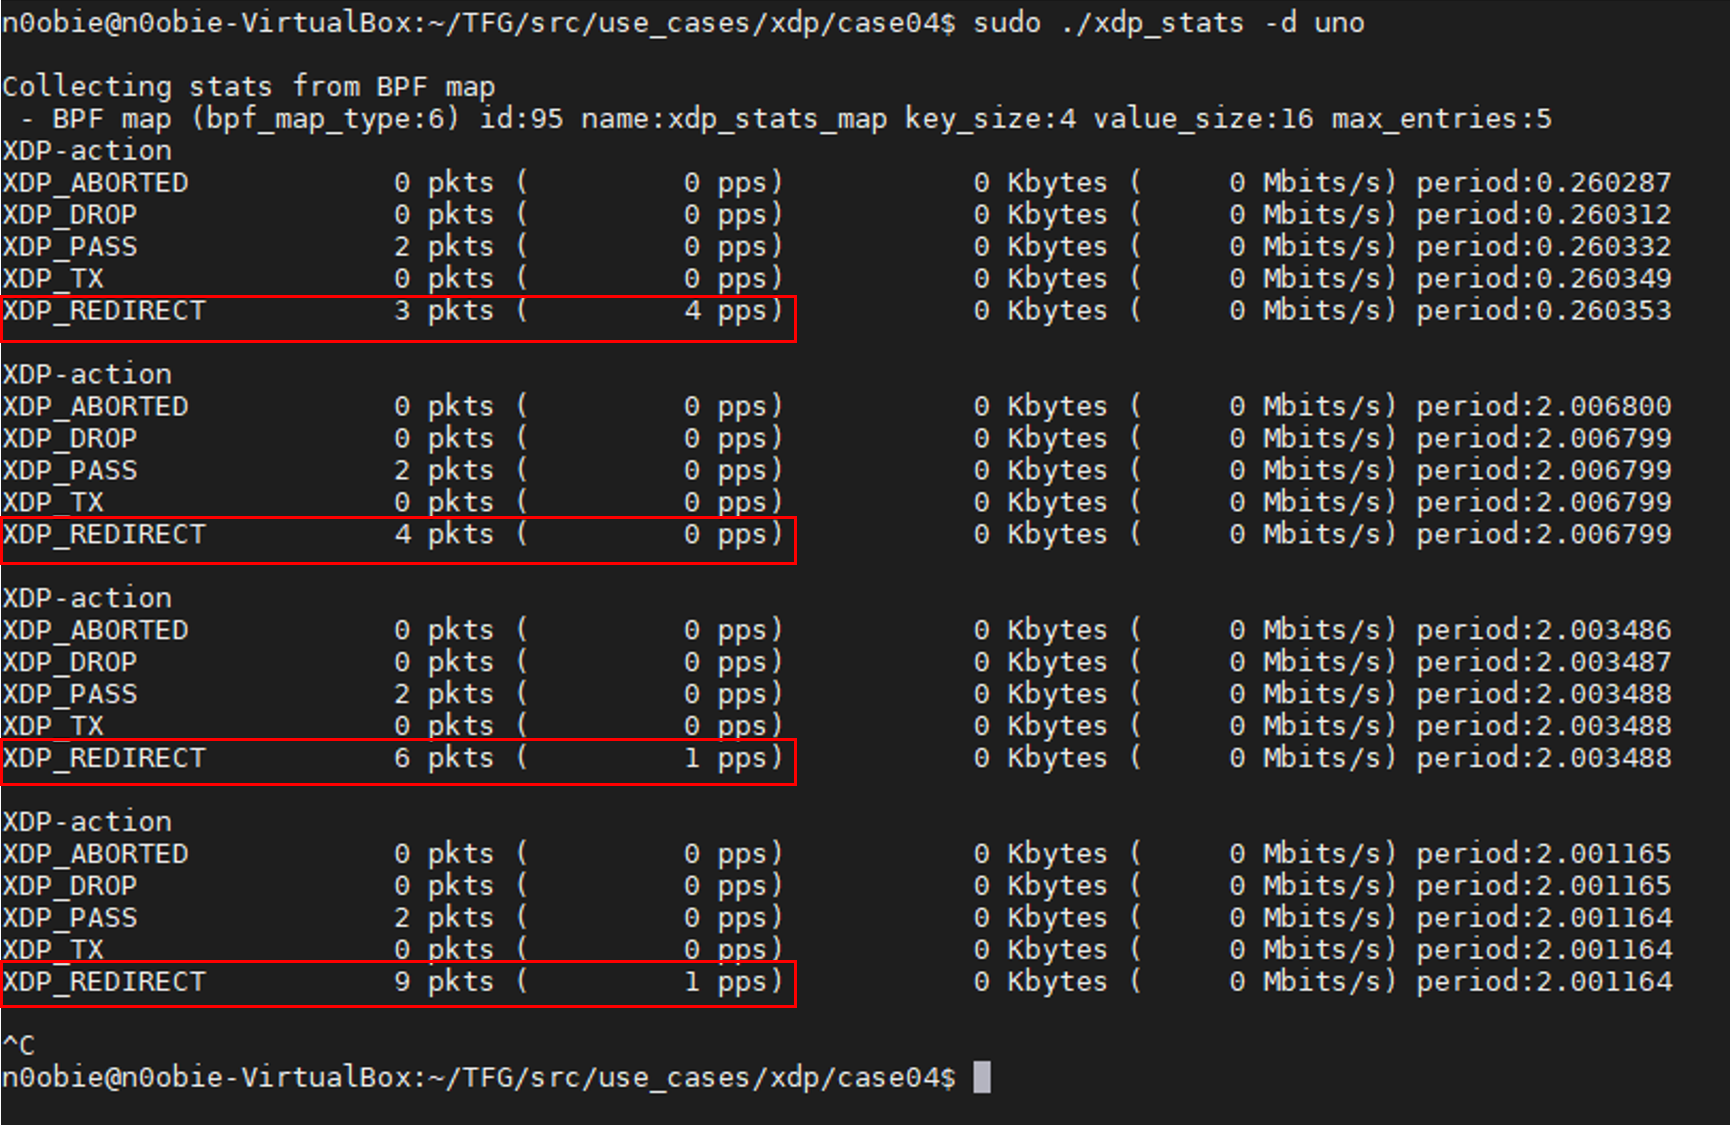
\includegraphics[width=14cm]{archivos/img/dev/xdp/case04/demo_case04_semihard_3_edited.png}
        \caption{Estadísticas de los códigos de retorno XDP}
        \label{fig:case04_xdp_ether_func2_stats}
    \end{subfigure}
    \caption{Comprobación de funcionamiento Semi-Hardcoded forwarding del Case04 - XDP}
    \label{fig:case04_xdp_ether_func2}
\end{figure}

% \todo{Cambiar este bloque de código por una imagen ya que es un resultado}
% \begin{lstlisting}[language= bash, style=Consola, caption={Comprobación del funcionamiento Semi-Hardcoded forwarding - Case04},label=code:case04_xdp_ether_func2]
%     # Hacemos un ping desde el interior de la Network namespace "uno" hacia la veth0 de la Network namespace "dos"
%     ping  {IP_veth_dos} [ y viceversa..]
    
%     # Comprobamos con el recolector de estadísticas que se están produciendo XDP_REDIRECT
%     sudo ./xdp_stats -d uno
    
%     ó
    
%     sudo ./xdp_stats -d dos
% \end{lstlisting}



%%%%%%%%%%%%%%%%%%%%%%%%%%%%%%%%%%%%%%%%%%%%%%%%%%%%%%%%%%%%%%%%%%%%%%%%%%%%%%%%%%%%
\subsubsection{Forwarding auto (Kernel FIBs)}

La tercera forma de hacer forwarding hace referencia al forwarding automático, esto es debido a que no habrá ningún tipo de información de forwarding hardcodeada en el programa \gls{xdp}, la información se obtendrá del propio \textit{stack} de red trabajando de forma cooperativa con éste. El escenario sobre el cual se trabajará será el mismo que el anterior por lo que únicamente es necesario preocuparse de limpiar el escenario de los programas \gls{xdp} anteriormente anclados a cada interfaz para que no interfieran con los nuevos programas \gls{xdp} que se van anclar.\\
\par
En este caso, se va a ir un paso más allá y el forwarding será automático, es decir, no se hardcodeará ningún tipo de información para hacer el forwarding a los paquetes. Pero, entonces: ¿cómo se sabrá a dónde hay que mandar los paquetes? Esta información se conseguirá del \textit{stack} de red del Kernel de Linux el cual tiene una FIB (\textit{Forwarding Information Base}) con reglas muy útiles las cuales se pueden sacar partido. \\
\par
Por lo que, se realizará una consulta a la FIB con el \textit{helper} \texttt{bpf\_fib\_lookup()} para obtener información de forwarding desde el propio \textit{stack} de red, este es un claro ejemplo donde la cooperación con el \textit{stack} de red hace que el programa \gls{xdp} sea más robusto e independiente del espacio de usuario.

% figura escenario
\begin{figure}[ht]
    \centering
    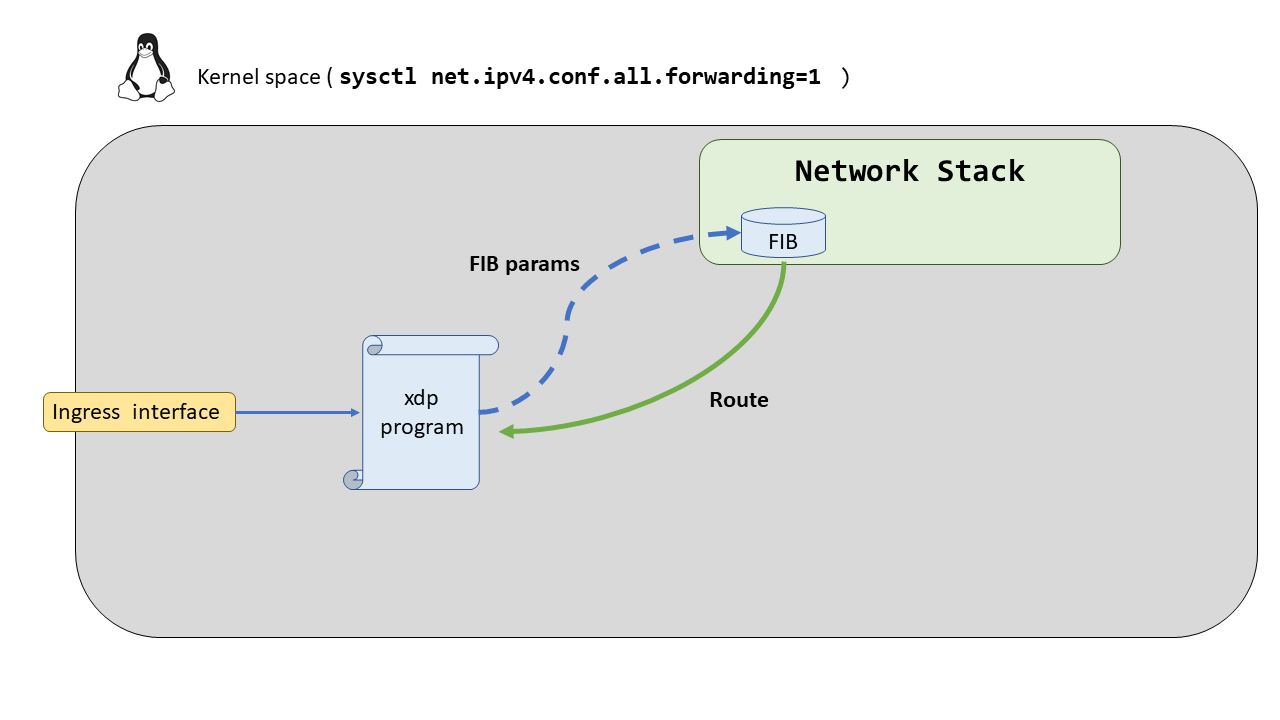
\includegraphics[width=16cm]{archivos/img/dev/xdp/case04/scenario_03.png}
    \caption{Escenario cableado Forwarding auto del Case04 - XDP}
    \label{fig:case04_xdp_ether_scenario3}
\end{figure}
\newpage
\vspace{1cm}
\textbf{Carga del programa XDP}\\
\par
Para la carga del programa \gls{xdp} se deberá primero habilitar el forwarding en nuestro Kernel, acto seguido se anclarán los \textit{dummy program} y por último, se anclarán anclar los programas \gls{xdp} en ambas interfaces tanto \texttt{uno} como \texttt{dos} para conseguir que la comunicación sea bidireccional.
\vspace{0.5cm}

\begin{lstlisting}[language= bash, style=Consola, caption={Carga del programa XDP Forwarding auto - Case04},label=code:case04_xdp_ether_load3]
    # Habilitamos el forwarding 
    sudo sysctl net.ipv4.conf.all.forwarding=1
    
    # Anclamos los programas XDP a cada interfaz 
    sudo ./xdp_loader -d uno -F --progsec xdp_case04_fib
    sudo ./xdp_loader -d dos -F --progsec xdp_case04_fib
    
    # Ahora añadimos a cada interfaz destino su "dummy program"
    sudo ip netns exec uno ./xdp_loader -d veth0 -F --progsec xdp_pass
    sudo ip netns exec dos ./xdp_loader -d veth0 -F --progsec xdp_pass
    
    # Habilitamos los ifindex 
    sudo ./prog_user -d uno
    sudo ./prog_user -d dos
\end{lstlisting}

\vspace{1cm}

\textbf{Comprobación del funcionamiento}\\
\par
La comprobación de funcionamiento de este programa puede ser llevada a cabo desde un extremo u otro debido a que, si todo funciona correctamente, existirá una comunicación bidireccional y completamente automática ya que no ha almacenado ningún tipo de información en los programas anclados. Por lo que, se harán las pruebas desde la \textit{Network namespace} \texttt{uno} hacia la \texttt{dos}. Como se puede apreciar en la figura \ref{fig:case04_xdp_ether_func3}, atendiendo al funcionamiento del ping \fcolorbox{black}{yellow}{\rule{0pt}{2.5pt}\rule{2.5pt}{0pt}}\hspace{1mm}, hay una perfecta comunicación entre ambas \textit{Network namespaces}, por lo que el programa está tomando correctamente las rutas de la FIB. \\

% \todo{Cambiar este bloque de código por una imagen ya que es un resultado}
\begin{lstlisting}[language= bash, style=Consola, caption={Comprobación del funcionamiento Forwarding auto - Case04},label=code:case04_xdp_ether_func3]
    # Hacemos un ping desde el interior de la Network namespace "uno" hacia la veth0 de la Network namespace "dos"
    ping  {IP_veth_dos} [ y viceversa..]
    
    # Comprobamos con el recolector de estadísticas que se están produciendo XDP_REDIRECT
    sudo ./xdp_stats -d uno

\end{lstlisting}

\newpage

\begin{figure}[h]
    \centering
    \begin{subfigure}[b]{\textwidth}
    	\centering
        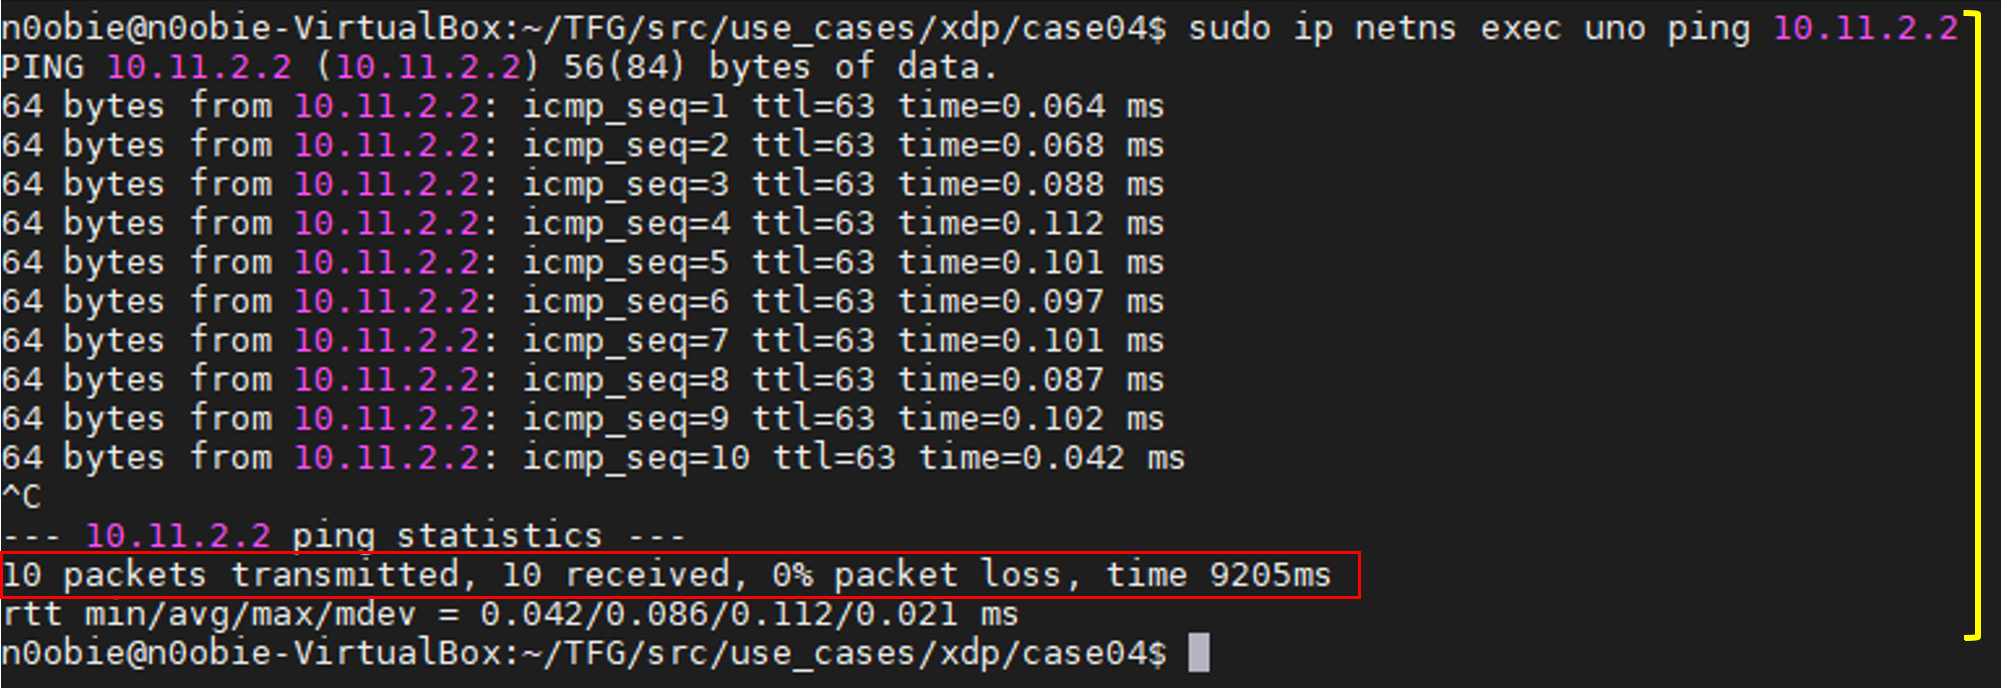
\includegraphics[width=13cm]{archivos/img/dev/xdp/case04/demo_case04_auto_2_edited.png}
        \caption{Ejecución de ping hacia la interfaz con el programa XDP}
        \label{fig:case04_xdp_ether_func3_ping}
    \end{subfigure}
    \par\bigskip
    \begin{subfigure}[b]{\textwidth}
    	\centering
        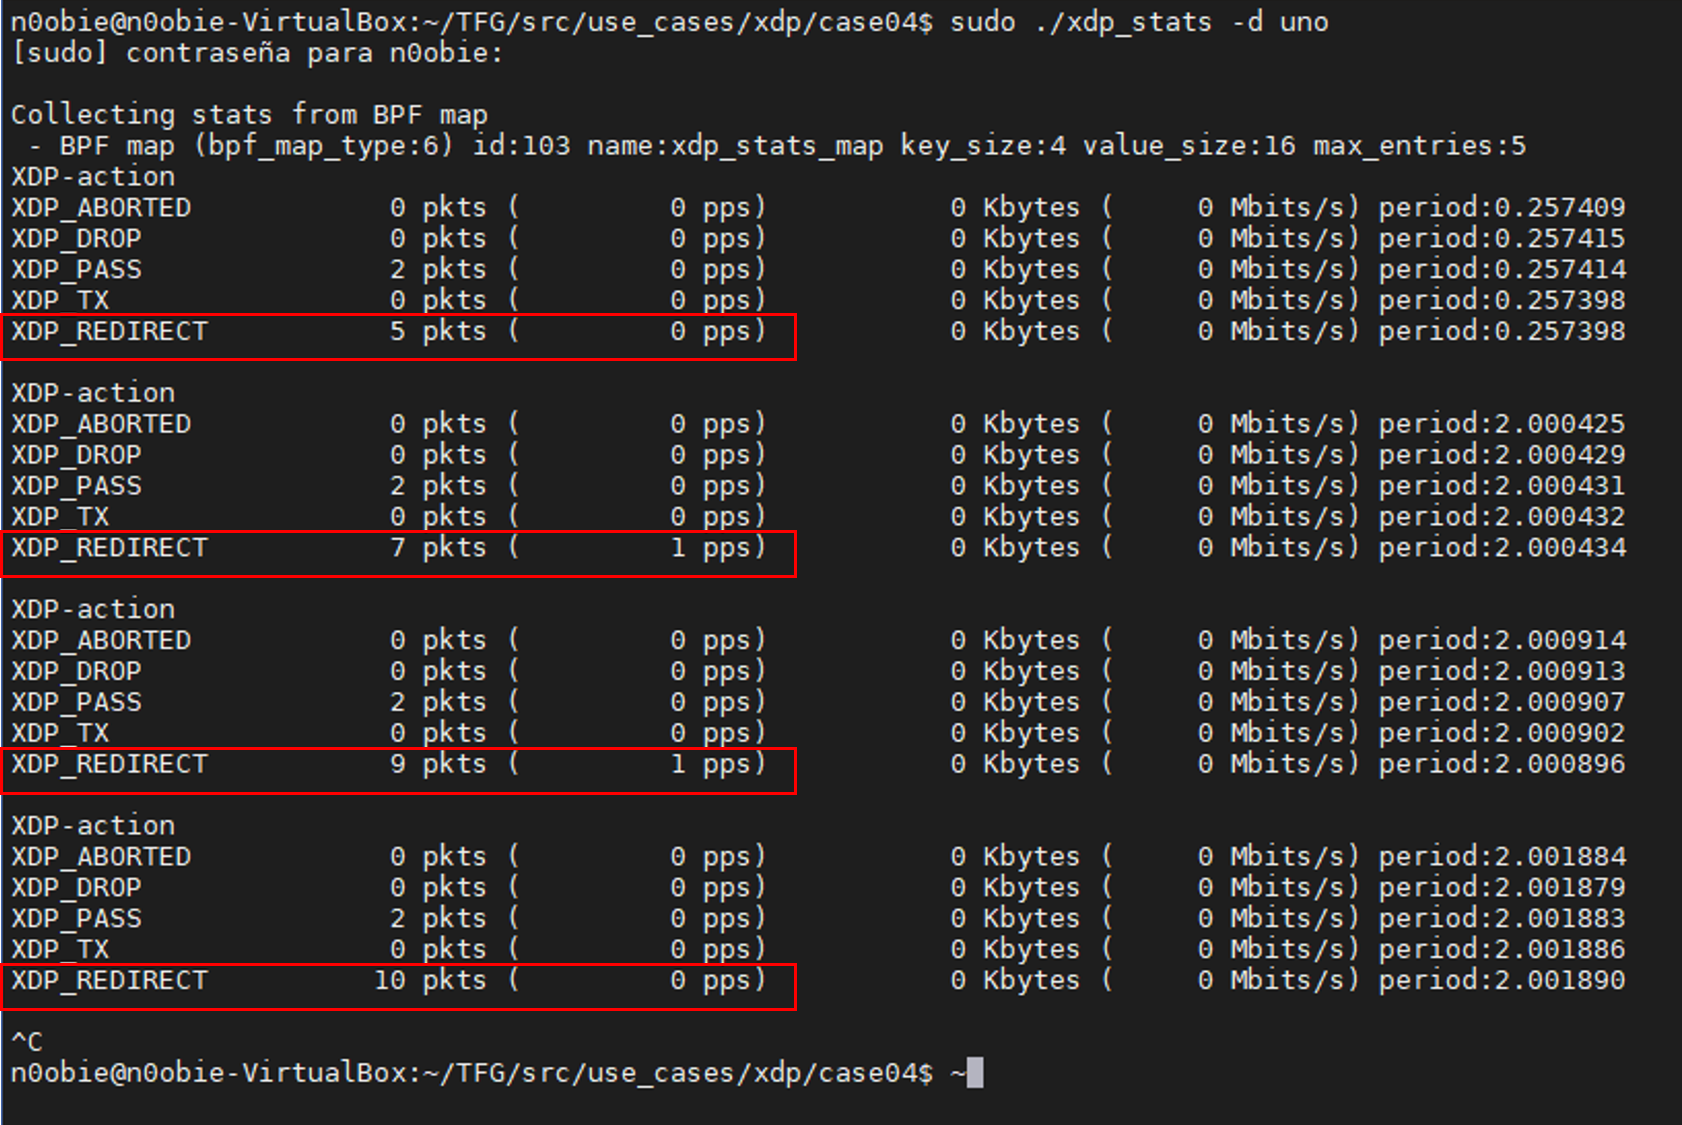
\includegraphics[width=14cm]{archivos/img/dev/xdp/case04/demo_case04_auto_3_edited.png}
        \caption{Estadísticas de los códigos de retorno XDP}
        \label{fig:case04_xdp_ether_func3_stats}
    \end{subfigure}
    \caption{Comprobación de funcionamiento Forwarding auto del Case04 - XDP}
    \label{fig:case04_xdp_ether_func3}
\end{figure}
\subsection{Case05 - Broadcast}
\label{xdp_ether_case05}

Por último, en este caso de uso se explorará la capacidad de reenvío a multiples interfaces de \gls{xdp}. Por ello, se ha intentado replicar un escenario básico de broadcast con \textit{Network Namespaces}. Se ha planteado hacer uso de la herramienta arping para emular una resolución ARP, generando paquetes ARP-Request. Dichos paquetes llevarán su MAC destino todo a \texttt{FF:FF:FF:FF:FF:FF} y su dominio de difusión englobaría todos aquellos nodos de la red que operen hasta capa 2. Como por ejemplo un hub, o un switch. En la figura \ref{fig:case05_xdp_ether_scenario1} se puede encontrar el escenario a recrear en este caso de uso.\\
\par
% figura escenario
\begin{figure}[ht]
    \centering
    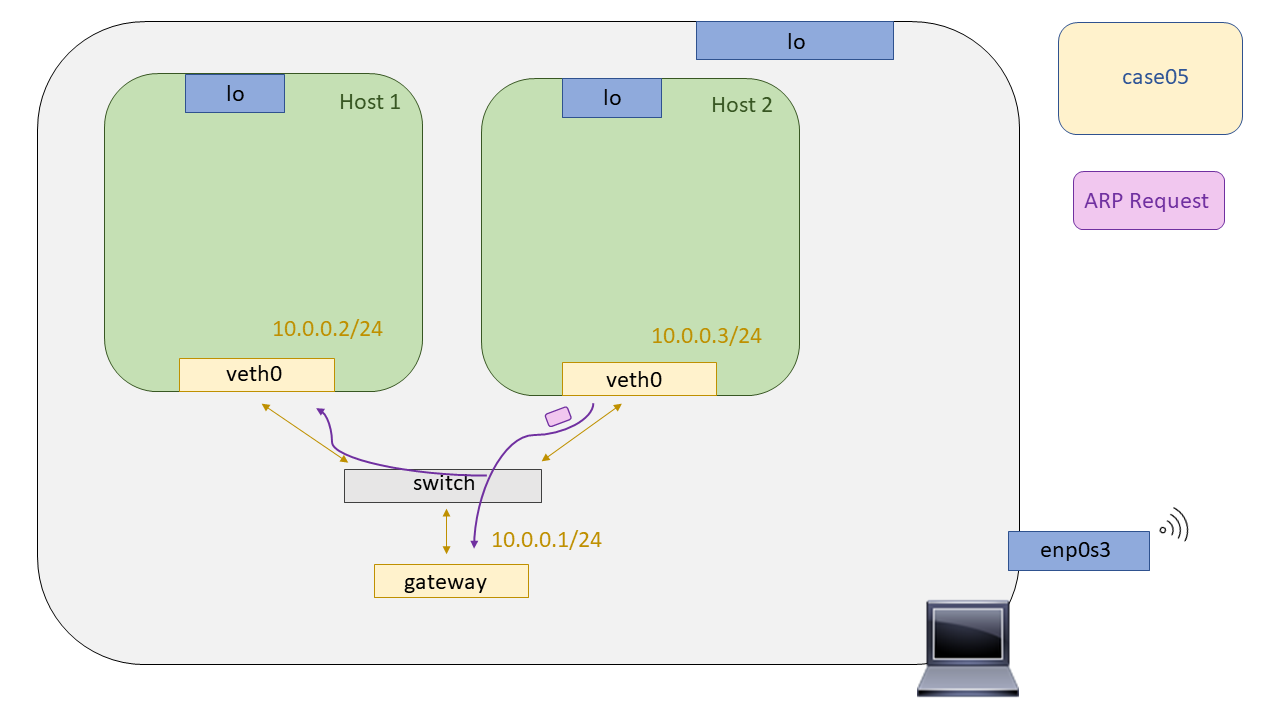
\includegraphics[width=14cm]{archivos/img/dev/xdp/case05/scenario_01.png}
    \caption{Escenario a recrear del Case05 - XDP}
    \label{fig:case05_xdp_ether_scenario1}
\end{figure}

El escenario propuesto para emular dicho escenario ha sido el siguiente (Ver figura \ref{fig:case05_xdp_ether_scenario2}). Este estaría compuesto de tres \textit{Network Namespaces} replicando así cada una de ellas un nodo independiente de la red, después, para intercomunicar cada ``nodo" de la red, se ha hecho uso de \gls{veth}s. El supuesto switch será la \textit{Network Namespace} llamada \texttt{switch}, la cual requerirá de un programa \gls{xdp} para poder actual como tal, ya que de no ser así sus interfaces tendrán todo el \textit{stack} de red de Linux por encima de ellas. Es decir, el nodo implementará todas las capas del modelo TCP/IP (DoD), replicando así la funcionalidad de un hipotético host y no actuando como un switch.\\
\par

% figura escenario
\begin{figure}[ht]
    \centering
    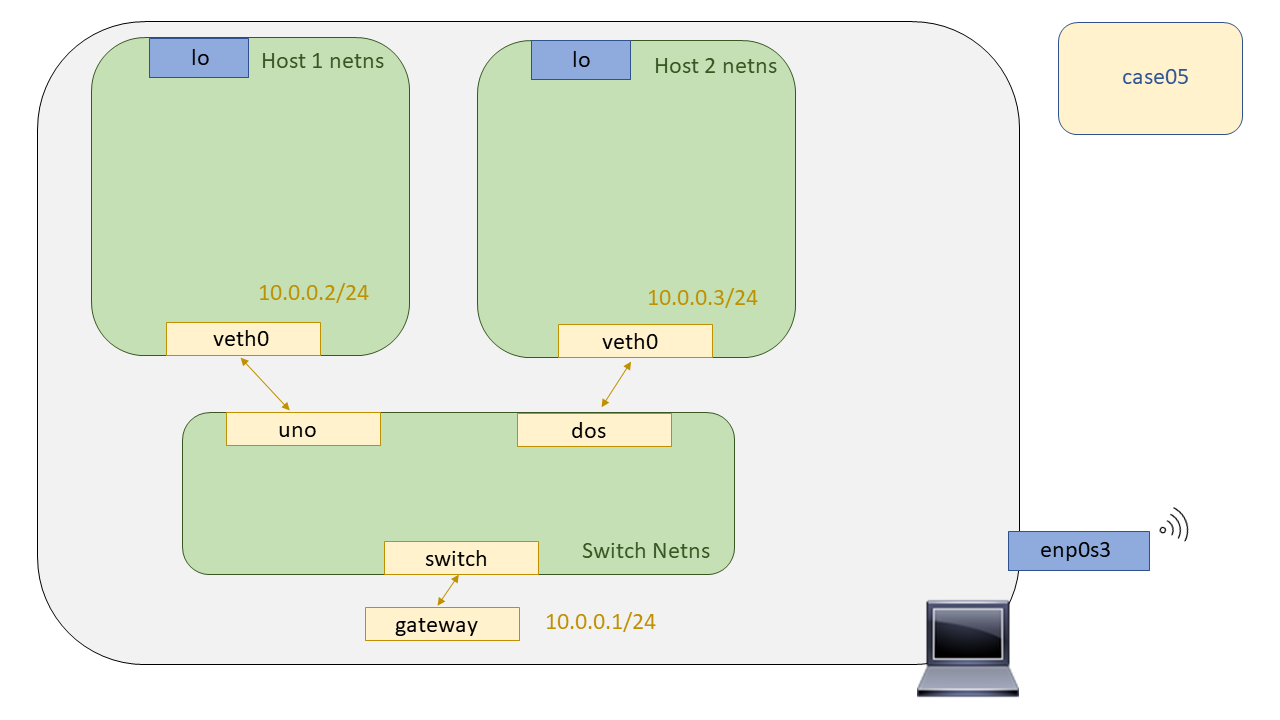
\includegraphics[width=16cm]{archivos/img/dev/xdp/case05/scenario_02.png}
    \caption{Escenario propuesto del Case05 - XDP}
    \label{fig:case05_xdp_ether_scenario2}
\end{figure}

Para realizar el broadcast se indagó sobre los \textit{helpers} \gls{bpf} en busca de alguna función que ayudara a satisfacer la necesidad, y se encontró una función (\ref{code:case05_xdp_ether_kernprog1}) que a primera vista se creía que podía ser de utilidad.

\begin{lstlisting}[language=C, style=C-color, caption={Helper BPF para realizar un Broadcast - Case05},label=code:case05_xdp_ether_kernprog1]
    int bpf_clone_redirect(struct sk_buff *skb, u32 ifindex, u64 flags);
\end{lstlisting}
\vspace{0.2cm}

Pero hubo un pequeño detalle que se pasó por alto, y es que requiere que el paquete ya se encuentre en una estructura \texttt{sk\_buff}. Es decir, podría surgir la siguiente cuestión: ¿qué implica que la función requiera de una estructura de datos \texttt{sk\_buff}? Antes de continuar con este caso de uso, se recomienda regresar a la sección \ref{linuxNetworking_skbuff} dónde se explica la estructura \texttt{sk\_buff}, para qué se utiliza y qué puede ofrecer.


\vspace{1cm}
\textbf{Restricciones para hacer Broadcast con XDP}\\
\par

Atendiendo a las características de la estructura \texttt{sk\_buff}, se pueden entender un poco mejor las restricciones que implica que el \textit{helper} \gls{bpf} haga uso de esta estructura. Cuando se trabaja con \gls{xdp}, se maneja una estructura mucho más simple y menos pesada que el \texttt{sk\_buff}, llamada \texttt{xdp\_buff}, en la que se introduce la información exclusiva para operar con el paquete en la propia interfaz.\\
\par

Por ello, no se puede hacer uso del \textit{helper} \gls{bpf} ya en caso de querer hacer uso de él se debería hacer una reserva para esta estructura y hacer una traducción a mano de \texttt{xdp\_buff} a \texttt{sk\_buff}. Haciendo esto se estaría operando de manera intrusiva con la lógica propia del \textit{stack} de red del Kernel de Linux, y además se estaría perdiendo el rendimiento que reporta no trabajar con estas estructuras.

Por lo que investigando y aprendiendo un poco más sobre \gls{bpf} para poder valorar las posibles opciones antes de desistir, se vio que el siguiente punto siguiendo el \textit{datapath} de Linux donde se producen ``\textit{hooks}" ( proceso de ancoraje de un \textit{bytecode} en el Kernel de Linux ) es en el \gls{tc}. Sabiendo cómo opera el \gls{tc} (en caso no ser así se recomienda la lectura de la
sección \ref{fig:linuxNet_tc}), se propone la siguiente solución para llevar a cabo el forwarding (Ver fig. \ref{fig:case05_xdp_ether_scenario3}).

% figura escenario
\begin{figure}[ht]
    \centering
    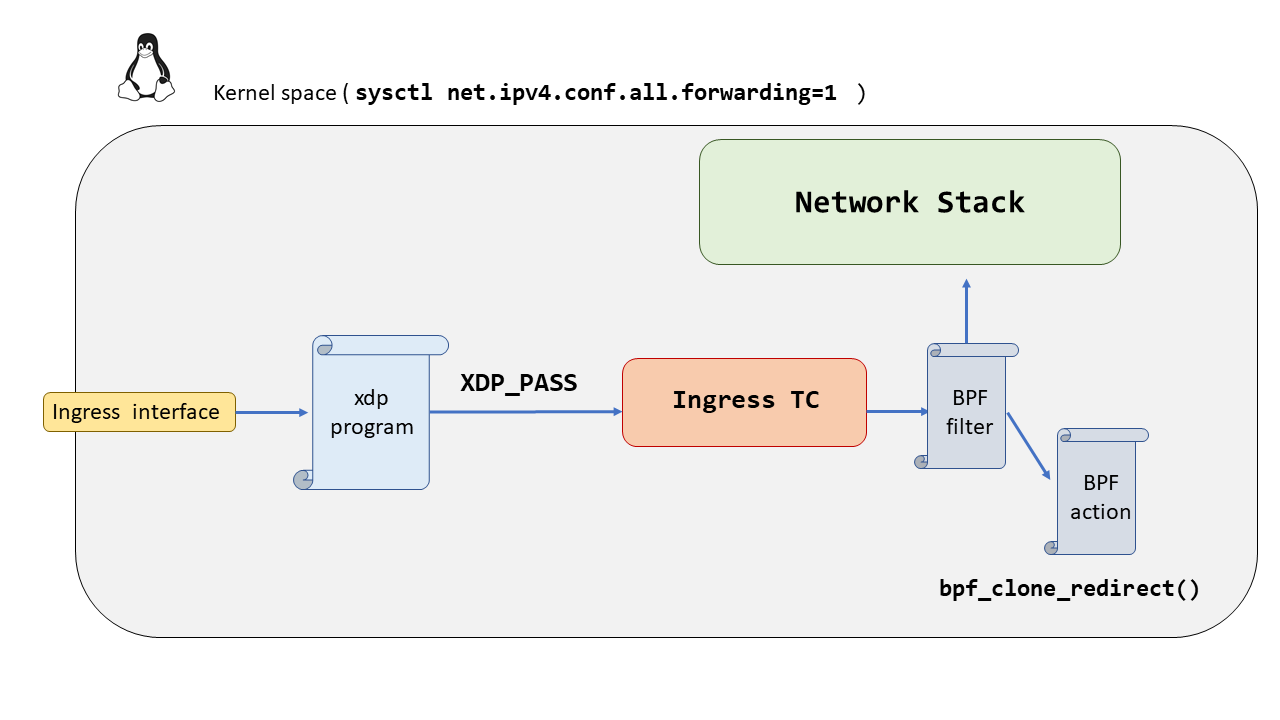
\includegraphics[width=16cm]{archivos/img/dev/xdp/case05/scenario_04.png}
    \caption{Solución propuesta para el Case05 - XDP}
    \label{fig:case05_xdp_ether_scenario3}
\end{figure}

De esta forma, en el \gls{tc} ya se tendría el manejo de la estructura \texttt{sk\_buff} y por ende, ya se podría hacer uso del \textit{helper} \gls{bpf} para clonar el paquete y hacer un reenvío a cada una de las interfaces que se quiera, para completar así el broadcast.


\vspace{1cm}
\textbf{Compilación}\\
\par

Para compilar el programa \gls{xdp} se ha dejado un Makefile preparado en este directorio al igual que en el case04 (\ref{xdp_ether_case04}), por lo que para compilarlo únicamente hay que seguir las indicaciones del bloque \ref{code:case04_xdp_ether_compilacion}.

\begin{lstlisting}[language= bash, style=Consola, caption={Compilación programa XDP - Case05},label=code:case05_xdp_ether_compilacion]
    # En caso de no haber entrado en el directorio asignado del caso de uso
    cd TFG/src/use_cases/xdp/case05
    
    
    # Hacemos uso del Makefile suministrado 
    sudo make
\end{lstlisting}
\vspace{0.5cm}

Si tiene dudas sobre el proceso de compilación del programa \gls{xdp} le recomendamos que vuelva al case02 (\ref{xdp_ether_case02}) donde se hace referencia al \textit{flow} dispuesto para la compilación de los programas \gls{xdp}.


\vspace{1cm}
\textbf{Puesta en marcha del escenario}\\
\par

Para comprobar el funcionamiento de los programas \gls{xdp} se hará uso de las \textit{Network Namespaces} (más información en la sección \ref{namespaces}). Como ya se comentaba, para que no suponga una barrera de entrada el concepto de las \textit{Network Namespaces}, se ha dejado escrito un script para levantar el escenario, y para su posterior limpieza. Es importante señalar que el script debe ser lanzado con permisos de root. Para levantar el escenario debemos ejecutar dicho script como se indica en el bloque \ref{code:case03_xdp_ether_escenario}.\\
\par
Para limpiar la máquina del escenario recreado anteriormente, se puede correr el mismo script indicándole ahora el parámetro \texttt{-c} (\textit{Clean}). En el peor de los casos, y si se cree que la limpieza se no se ha realizado de manera satisfactoria, se puede llevar a cabo un reinicio de la máquina consiguiendo así que todos los entes no persistentes (\gls{veth}, netns..) desaparezcan del equipo.

\begin{lstlisting}[language= bash, style=Consola, caption={Puesta en marcha del escenario - Case05},label=code:case05_xdp_ether_escenario]
    # Para levantar el escenario (Importante hacerlo con permisos de super usuario)
    sudo ./runenv.sh -i
    
    
    # Una vez finalizado la comprobación del caso de uso, limpiaremos nuestra maquina:
    sudo ./runenv.sh -c
\end{lstlisting}
\vspace{0.5cm}
Una vez levantado el escenario, tendríamos el escenario que se muestra en la figura \ref{fig:case05_xdp_ether_scenario4} montado con tres \textit{Network Namespaces} y pares de \gls{veth}s para interconectarlas. Los programas irán anclados a las interfaces de la \textit{Network Namespace} \texttt{switch}.
% figura escenario
\begin{figure}[ht]
    \centering
    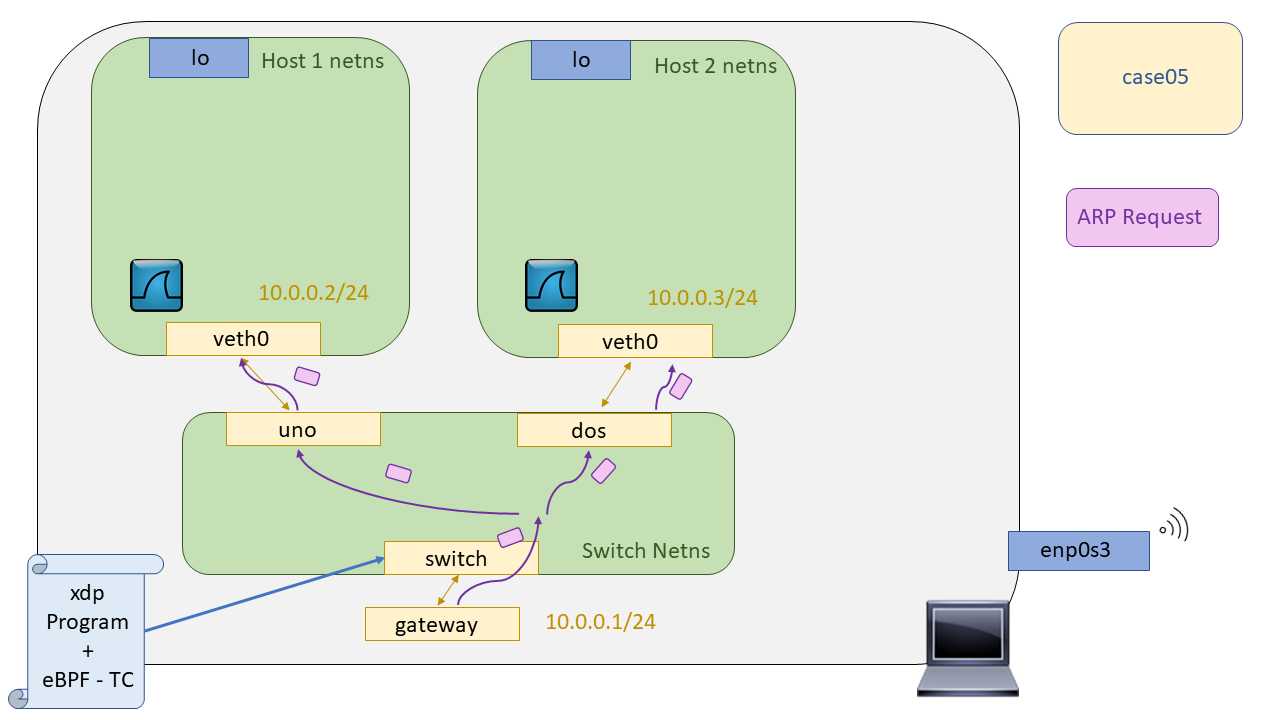
\includegraphics[width=16cm]{archivos/img/dev/xdp/case05/scenario_03.png}
    \caption{Escenario del Case05 - XDP}
    \label{fig:case05_xdp_ether_scenario4}
\end{figure}

\vspace{1cm}
\textbf{Carga del programa XDP}\\
\par
Una vez compilado tanto el programa \gls{xdp} como los programas \gls{bpf} que irán al \gls{tc}, es hora de cargarlos. Por lo que, para hacerlo y por mayor comodidad se abrirá un proceso de bash en la \textit{Network Namespace} switch. Acto seguido, se cargará el programa \gls{xdp}, y se incluirán los programas \gls{bpf} añadiendo una nueva qdisc con un filtro \gls{bpf} asociado que derivará en una acción. Dicha acción, será otro programa \gls{bpf} con la función de clonar los paquetes y mandarlos a otras interfaces.\\
\par
\begin{lstlisting}[language= bash, style=Consola, caption={Carga del programa XDP - Case05},label=code:case05_xdp_ether_load]
    # Nos abrimos un proceso de bash sobre la Network Namespace "switch"
    sudo ip netns exec switch bash
    
    # Cargamos el programa XDP_PASS
    sudo ./xdp_loader -d switch xdp_pass
    
    # Creamos la nueva qdisc
    sudo tc qdisc add dev switch ingress handle ffff:
    
    # Aplicamos a la qdisc creada un filtro BPF que en caso de matchear aplicará una acción (Otro programa BPF que hará nuestro broadcast)
    sudo tc filter add dev switch parent ffff: bpf obj bpf.o sec classifier flowid ffff:1 action bpf obj bpf.o sec action 
\end{lstlisting}

\vspace{1cm}
\textbf{Comprobación del funcionamiento}\\
\par
Para comprobar el funcionamiento del sistema de broadcast se realizará la siguiente prueba, donde desde la \textit{Network Namespace} por defecto se generarán ARP-Request hacia la IP de una de las \gls{veth}s de las \textit{Network Namespace} destino. \\
\par

Si el sistema de broadcast funciona correctamente, escuchando en las \textit{Network Namespace} destino \texttt{uno} y \texttt{dos}, se debería ver como los paquetes ARP-Request llegan sin problemas. Solo el ``Host" al cual iban dirigidos los ARP-Request será el que intentará contestarlos sin éxito al haber implementado un sistema unidireccional. Para solucionar esta limitación se propone hacer uso de los programas \gls{xdp} desarrollados en case04 (\ref{xdp_ether_case04}) para conseguir una comunicación bidireccional.\\
\par
\begin{lstlisting}[language= bash, style=Consola, caption={Comprobación del funcionamiento - Case05},label=code:case05_xdp_ether_func]
    # Generamos el ARP-REQUEST
    arping 10.0.0.2/3
    
    # Escuchamos en las Network Namespace destino a la espera de ver ARP-REQUEST.
    sudo ip netns exec uno tcpduml -l
    sudo ip netns exec dos tcpduml -l
\end{lstlisting}
\vspace{0.5cm}

En este caso no se podrá hacer uso del programa xdp\_stats para ver si realmente los programas \gls{xdp} están funcionando como se quiere que funcionen, ya que la lógica de broadcast se encuentra en el programa \gls{bpf} anclado como acción en un filtro del \gls{tc}.\\
\par
Como se puede apreciar en la figura \ref{fig:case05_xdp_ether_func}, los ARP-Request \fcolorbox{black}{green}{\rule{0pt}{2.5pt}\rule{2.5pt}{0pt}}\hspace{1mm} llegan a ambos Host, y solo aquel al cual iba dirigida la resolución ARP contesta. Pero como ya se comentaba antes, al no haber implementado un sistema de forwarding, la comunicación únicamente está planteada en un sentido.\\
\par
Esta funcionalidad se podría aumentar haciendo uso de los programas desarrollados en el caso de uso anterior (\ref{xdp_ether_case04}). Por lo que se concluye afirmando que se ha podido hacer broadcast, pero no de forma exclusiva con \gls{xdp} ya que se ha tenido que añadir \gls{bpf} nativo en el \gls{tc}.

% figura escenario
\begin{figure}[ht]
    \centering
    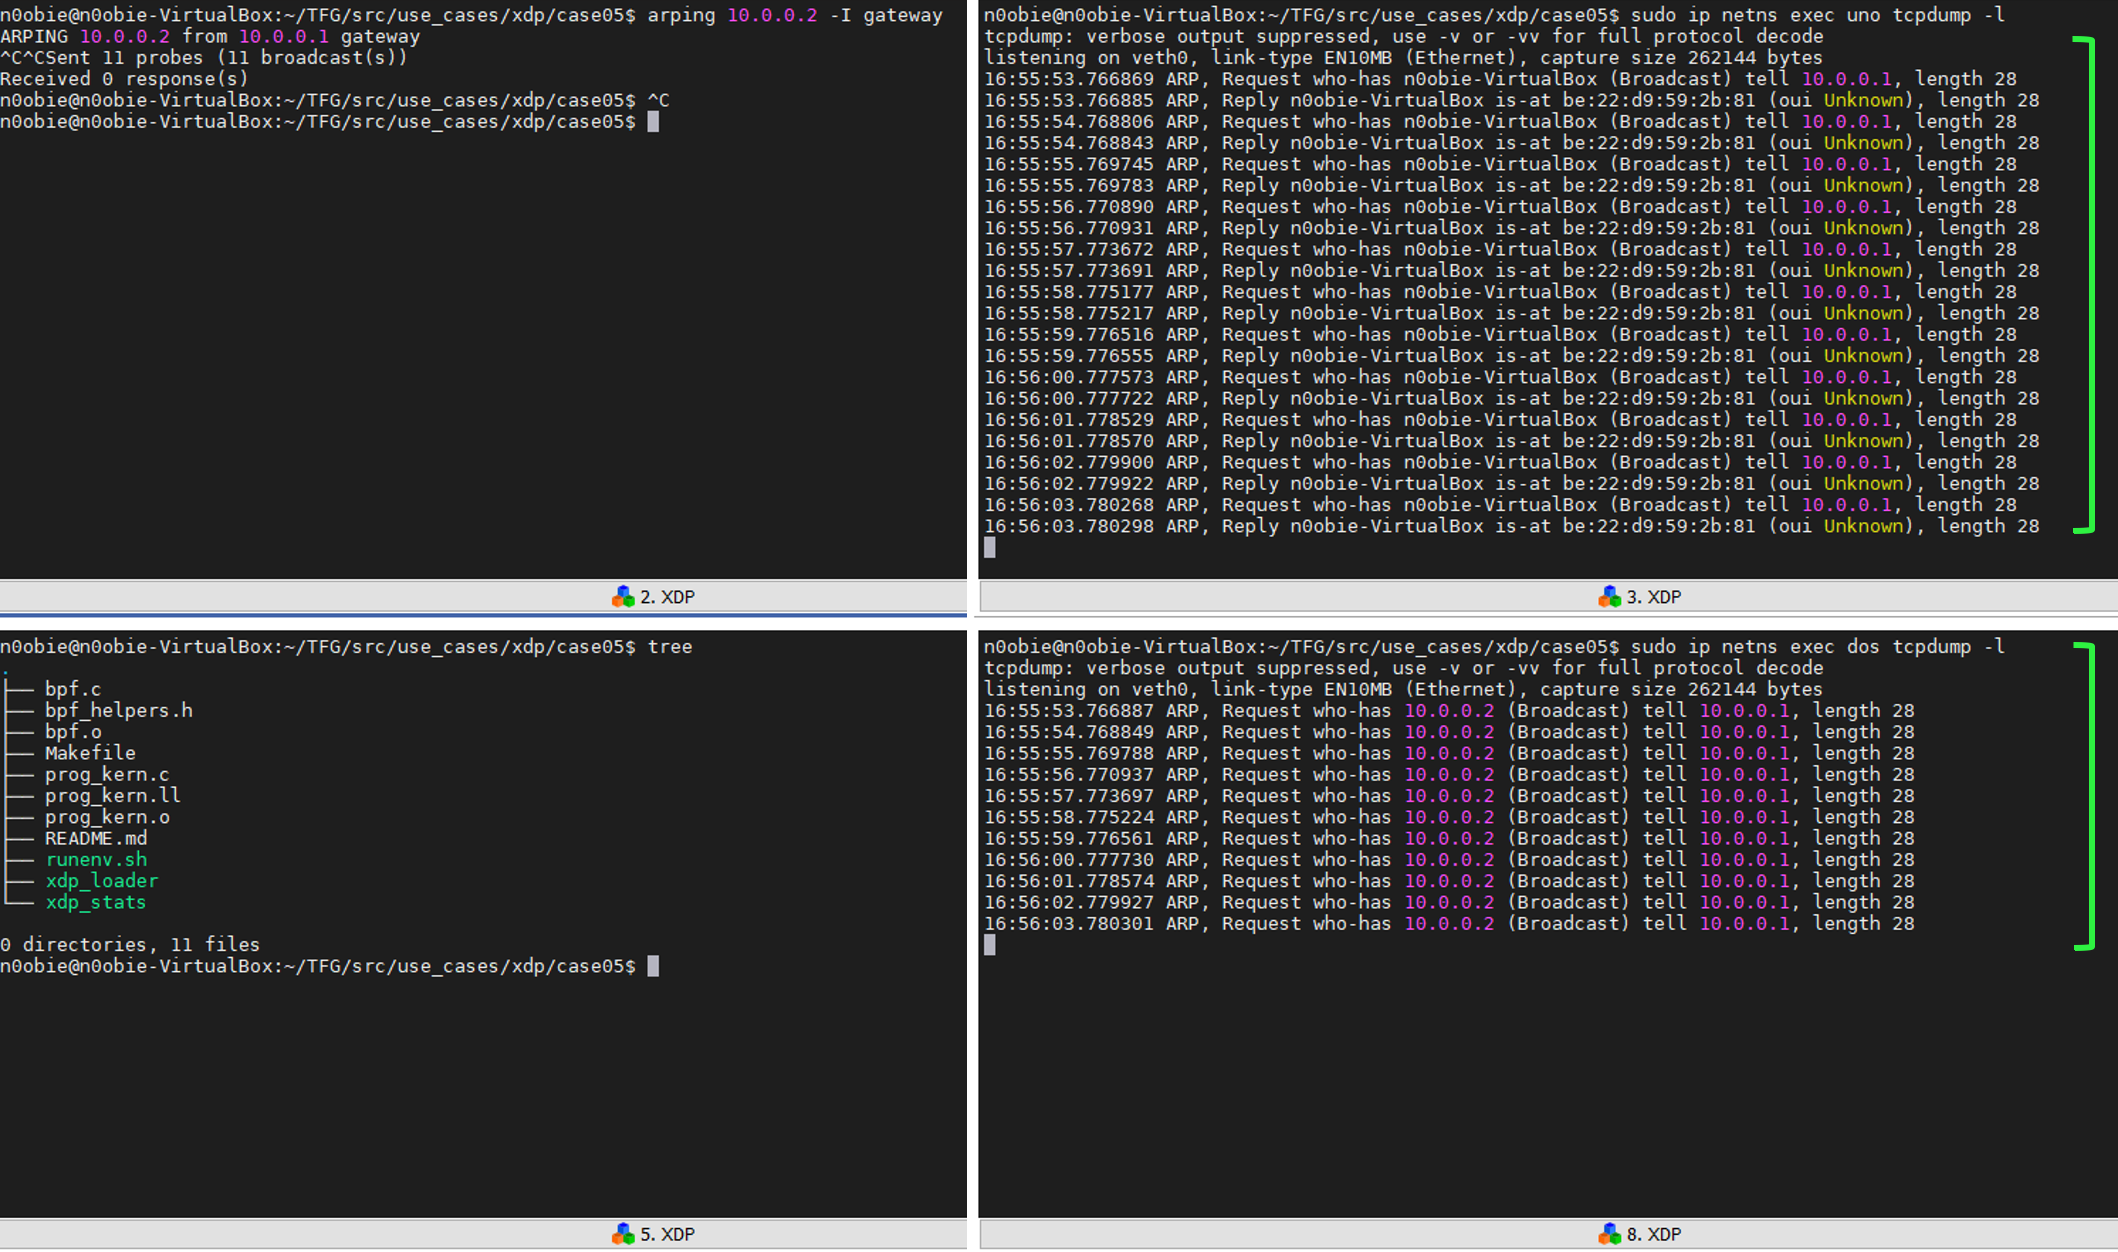
\includegraphics[width=16cm]{archivos/img/dev/xdp/case05/demo_case05_edited.png}
    \caption{Comprobación de funcionamiento del Case05 - XDP}
    \label{fig:case05_xdp_ether_func}
\end{figure}
\newpage


%%%%%%%%%%%%%%%%%%%%%%%%%%%%%%%%%%%%%%%%%%%%%%%%%%%%%%%%%%%%%%%%%%%%%%%%%%%%%%%%%%%%%%%%%%%%%%%

\section{Casos de uso P4 en medios cableados}

En esta sección se introducirán todos los casos de uso realizados con la tecnología P4 en entornos cableados. Todos los casos de uso se han nombrado siguiendo la misma sintaxis que en el repositorio del \gls{tfg}, alojado en GitHub. Para \textbf{la instalación de las dependencias} de la tecnología P4, se ha generado el Anexo \ref{deps} donde se detallan todos los pasos a seguir. Se advierte al lector que quiera replicar los casos de uso, que  debe ser extremadamente cuidadoso con las dependencias del entorno P4 que instala, ya que, de querer hacer un \textit{upgrade} alguna de ellas puede generar numerosas incompatibilidades. \\
\par

Los casos de uso P4, al igual que con los casos de uso \gls{xdp}, se han dividido en partes diferenciadas con la finalidad de que la lectura de estos sea más clara y ordenada.

\begin{itemize}
    \item \textbf{Introducción}: En esta parte se abordarán las explicaciones teóricas complementarias, explicaciones propias sobre el caso de uso y comentarios sobre el código P4 desarrollado.
    
    \item \textbf{Compilación y puesta en marcha del escenario}: En esta parte se explicará al lector cómo proceder para compilar el programa P4 y cómo levantar el escenario. En este caso ambos procesos están integrados en un mismo Makefile, por lo que, la replicación los casos de uso será más amena.
    
    \item \textbf{Evaluación del funcionamiento}: Por último, se hará una evaluación sobre el funcionamiento del caso de uso empleando la CLI de Mininet.
\end{itemize}

Para que el lector pueda seguir el desarrollo de los casos de uso P4, a continuación se indica la tabla \ref{tab:P4_ether_usecases}, la cual expone en qué ruta del repositorio del \gls{tfg} se puede encontrar dicho caso de uso, y un vídeo demostración donde el autor va comentando paso a paso el caso de uso y su evaluación. \\
\par
\vspace{0.2cm}
\begin{table}[ht]
\centering
\resizebox{\textwidth}{!}{%
\begin{tabular}{|l|c|c|}
\hline
\rowcolor[HTML]{EFEFEF} 
\multicolumn{1}{|c|}{\cellcolor[HTML]{EFEFEF}\textbf{Caso de uso}} & \textbf{Enlace al repositorio} & \textbf{Enlace al vídeo demostración  } \\ \hline
case01 - Drop                                                      & \href{https://github.com/davidcawork/TFG/tree/master/src/use_cases/p4/case01}{\texttt{Enlace al código}}                         & \href{https://youtu.be/RKdi6SC5jYQ}{Enlace al vídeo}                                \\ \hline
case02 - Pass                                                      & \href{https://github.com/davidcawork/TFG/tree/master/src/use_cases/p4/case02}{\texttt{Enlace al código}}                         & \href{https://youtu.be/5X78simgC60}{Enlace al vídeo}                                \\ \hline
case03 - Echo server                                               & \href{https://github.com/davidcawork/TFG/tree/master/src/use_cases/p4/case03}{\texttt{Enlace al código}}                          & \href{https://youtu.be/H8R6T_W34gM}{Enlace al vídeo}                                \\ \hline
case04 - Layer 3 forwarding                                        & \href{https://github.com/davidcawork/TFG/tree/master/src/use_cases/p4/case04}{\texttt{Enlace al código}}                           & \href{https://youtu.be/La-_JCXut1Y}{Enlace al vídeo}                                \\ \hline
case05 - Broadcast                                                 & \href{https://github.com/davidcawork/TFG/tree/master/src/use_cases/p4/case05}{\texttt{Enlace al código}}                          & \href{https://youtu.be/jExo0mj8t6k}{Enlace al vídeo}                                \\ \hline
\end{tabular}
}
\caption{Resumen de la documentación sobre los casos de uso P4 en entornos cableados}
\label{tab:P4_ether_usecases}
\end{table}
\vspace{0.5cm}
En esta ocasión, como ya se comentaba en el capitulo de Análisis y Diseño (\ref{analisisPreimplementacion}), la plataforma que se utilizará para evaluar el funcionamiento de los programas P4 en entornos cableados será Mininet. Por lo que si usted no está familiarizado con la herramienta Mininet, se le recomienda que acuda a la sección \ref{mininet} donde se hace una introducción a esta herramienta.

\newpage

%%%%%%%%%%%%%%%%%%%%%%%%%%%%%%%%%%%%%%%%%%%%%%%%%%%%%%%%%%%%%%%%%%%%%%%%%%%%%%%%%%%%%%%%
%   Casos de uso P4 medio Cableados
\subsection{Case01 - Drop}
\label{p4_ether_case01}
En este caso de uso se probará que es posible descartar todos los paquetes recibidos con un programa P4. Como tal, el programa P4 no es suficiente para probar esta funcionalidad, ya que requiere de una plataforma que sea capaz de soportar el lenguaje P4. Según se comentó en el capítulo de Análisis y Diseño (Cap. \ref{analisisPreimplementacion}), se hará uso de soft-switch llamado behavioral-model, \gls{bmv2} en adelante, para testear los programas P4 y de Mininet como escenario para recrear las topologías de Red. \\
\par

Antes de continuar con el caso de uso, se quiere remarcar un detalle importante. Continuamente se estará refiriendo al \gls{bmv2} como un ``switch", pero se debe entender que con el lenguaje P4 estamos definiendo el \textit{datapath} que tendrá la entidad que cargue con el programa P4, en este caso el  \gls{bmv2}. Por lo que, la denominación de switch puede no ser totalmente correcta, ya que depende del programa P4 que porte para comportarse como un switch. Nótese que el uso del término ``switch" deriva de la denominación de dispositivos programables en entornos SDN, que tradicionalmente se nombraron como ``switches" \\
\par

Debido a esto, el \gls{bmv2} puede actuar como un hub, un switch, un router o un firewall, etc. Dependerá de la funcionalidad implementada en el programa P4. Se aprovechará la interfaz implementada del \gls{bmv2} con Mininet, desarrollada desde la equipo de p4Lang, para conseguir integrar estos nodos en el escenario de red pudiendo así comprobar el funcionamiento del programa P4 desarrollado.\\
\par

\vspace{0.2cm}
\textbf{Compilación y puesta en marcha del escenario}\\
\par

Para la compilación del programa P4 se hará uso del compilador p4c. Este es el compilador de referencia para el lenguaje P4, es modular y permite escoger distintos \textit{targets} para llevar a cabo la compilación. El proceso de compilación de los programas P4 se lleva a cabo en dos etapas, una etapa de compilación de \textit{frontend} donde se genera un archivo \texttt{*.p4info}, el cual recoge todos los atributos necesarios del programa P4 en tiempo de ejecución ( identificadores de tablas, su estructura, \textit{actions}.. ), y una etapa de \textit{backend}, en la cual se hace uso del archivo generado \texttt{*.p4info} para generar los archivos necesarios para programar al \textit{target} en cuestión.\\
\par

% figura escenario
\begin{figure}[ht]
    \centering
    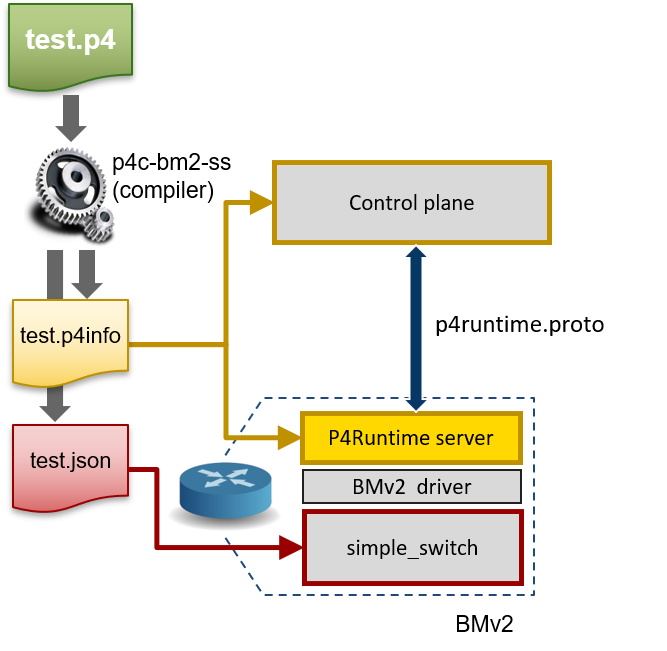
\includegraphics[width=5cm]{archivos/img/dev/p4/case01/compilation_bmv2.png}
    \caption{Proceso de compilación programa P4}
    \label{fig:case01_p4_ether_intro}
\end{figure}

Por ejemplo, el compilador de \textit{backend} que ataca al BMV2 genera un fichero \texttt{*.json}. Este fichero será suficiente para establecer todo el \textit{datapath} según lo programado en el programa P4. El target del compilador p4c que se utilizará es el \texttt{p4c-bm2-ss}, P4 simple\_switch - bmv2, el cual soporta la arquitectura \textbf{v1model}.\\
\par
Con la finalidad de poner en marcha del escenario, se ha dejado escrito un Makefile, el cual compilará el programa P4, generando los ficheros \texttt{*.p4info} y \texttt{*.json}. Acto seguido, se lanzará el script llamado \texttt{run\_exercise.py}, el cual levantará toda la topología descrita en el fichero \texttt{scenario/topology.json} con Mininet. Cada ``switch" de la topología tendrá implementada toda la lógica descrita en el programa P4 dentro de una instancia del \gls{bmv2}. A continuación, en la figura \ref{fig:case01_p4_ether_intro2} se puede ver una imagen resumen del levantamiento de un único ``switch".\\
\par
\vspace{0.5cm}
% figura escenario
\begin{figure}[ht]
    \centering
    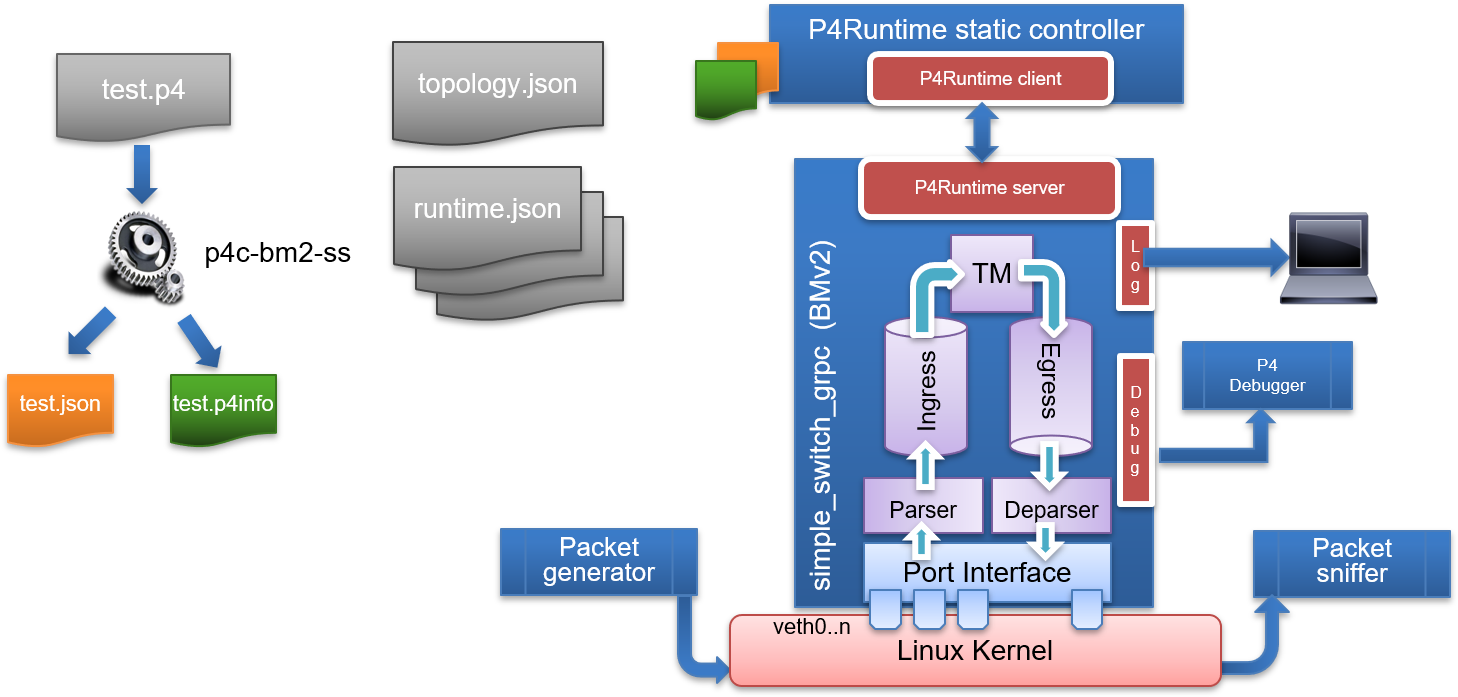
\includegraphics[width=15cm]{archivos/img/dev/p4/case01/setup.png}
    \caption{Proceso puesta en marcha de un switch BMv2 \cite{p42}}
    \label{fig:case01_p4_ether_intro2}
\end{figure}

\vspace{0.5cm}

Debido a que las personas que quieran replicar los casos de uso puede que no estén muy familiarizadas con todo este proceso de compilación y carga en los procesos de \gls{bmv2}, se ha dispuesto un de un Makefile para automatizar las tareas de compilación y carga de los programas, y también, para las tareas de limpieza del caso de uso una vez finalizada su demostración. Entonces, para proceder con la puesta en marcha del caso de uso, se deben seguir los pasos indicados en el bloque \ref{code:case01_p4_ether_load}.

\newpage

\begin{lstlisting}[language= bash, style=Consola, caption={Compilación programa P4 y puesta en marcha del escenario  - Case01},label=code:case01_p4_ether_load]
    # Entramos al directorio 
    cd TFG/src/use_cases/p4/case01

    # Hacemos uso del Makefile
    sudo make run
\end{lstlisting}
\vspace{0.5cm}

% figura escenario
\begin{figure}[ht]
    \centering
    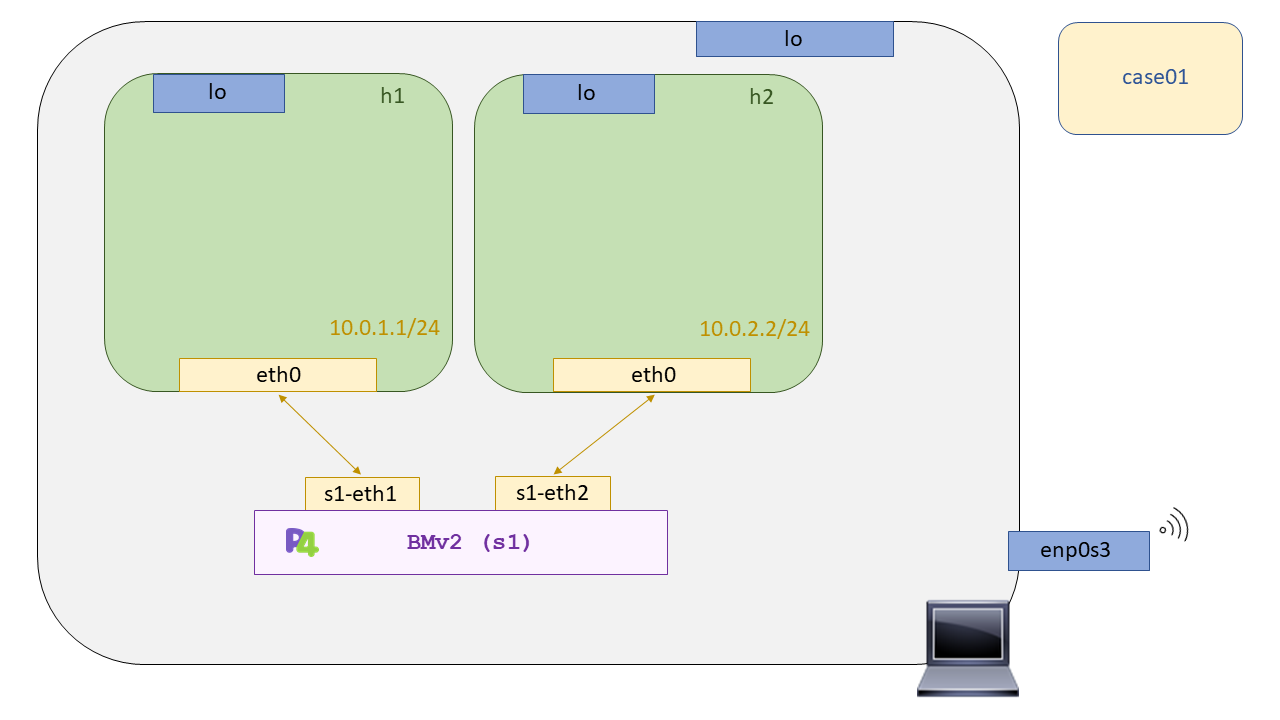
\includegraphics[width=16cm]{archivos/img/dev/p4/case01/scenario.png}
    \caption{Escenario del Case01 - P4}
    \label{fig:case01_p4_ether_scenario}
\end{figure}

Una vez se haya finalizado la comprobación del funcionamiento del caso de uso, se debe hacer uso de otro target (\textit{clean}) del Makefile para limpieza total del directorio.

\begin{lstlisting}[language= bash, style=Consola, caption={Limpieza del escenario P4 - Case01},label=code:case01_p4_ether_unload]
    # Hacemos uso del Makefile
    sudo make clean
\end{lstlisting}
\vspace{0.5cm}
Es importante señalar que este target limpiará tanto los ficheros auxiliares para la carga del programa P4 en el \gls{bmv2}, como los directorios de \texttt{pcaps}, \texttt{log}, y \texttt{build} generados en la puesta en marcha del escenario. Por lo que, si se desea conservar las capturas de las distintas interfaces de los distintos \gls{bmv2}, se deben copiar o limpiar del escenario a mano siguiendo las indicaciones del bloque \ref{code:case01_p4_ether_unload2}.

\begin{lstlisting}[language= bash, style=Consola, caption={Limpieza segura del escenario P4 - Case01},label=code:case01_p4_ether_unload2]
    # Limpiamos Mininet
    sudo mn -c
    
    # Limpiamos los directorios generados dinámicamente en la carga del escenario
    sudo rm -rf build logs
\end{lstlisting}


\vspace{0.5cm}
\textbf{Comprobación del funcionamiento}\\
\par

Una vez realizado el \texttt{make run} en este directorio, se tendrá levantada la topología descrita para este caso de uso, la cual se puede apreciar en la figura \ref{fig:case01_p4_ether_scenario}. La topología de este caso de uso se compondrá de una instancia del \gls{bmv2} (\texttt{s1}), y de dos host (\texttt{h1}, \texttt{h2}) que se conectarán al ``switch". Como ya se comentaba anteriormente, la topología puede encontrarse descrita bajo el directorio \texttt{scenario}, en un fichero JSON llamado \texttt{topology.json}. En este fichero también se describe la localización de los archivos que describen el plano de control de cada ``switch" de la topología. En todos los casos de uso, se ha respetado los nombres tipo utilizados por la organización de p4Lang, \texttt{sX-runtime.json}, donde X es el número que ocupa dicho switch en la topología de Mininet. Volviendo de nuevo a la comprobación del funcionamiento del caso de uso, se tendrá la CLI de Mininet abierta, por lo que se abrirá una terminal para el \texttt{host1} y otra para el \texttt{host2}.

\begin{lstlisting}[language= bash, style=Consola, caption={Comprobación de funcionamiento - Case01},label=code:case01_p4_ether_func]
    mininet>  xterm h1 h2
\end{lstlisting}
\vspace{0.5cm}

Ahora con ambas terminales abiertas, desde el \texttt{h2} se pondrá a escuchar por su interfaz. Se puede utilizar wireshark, o el sniffer que el lector crea conveniente. En este caso por simplicidad y no disponer de una interfaz gráfica, se utilizará tcpdump (\ref{tcpdump}).

% figura escenario
\begin{figure}[ht]
    \centering
    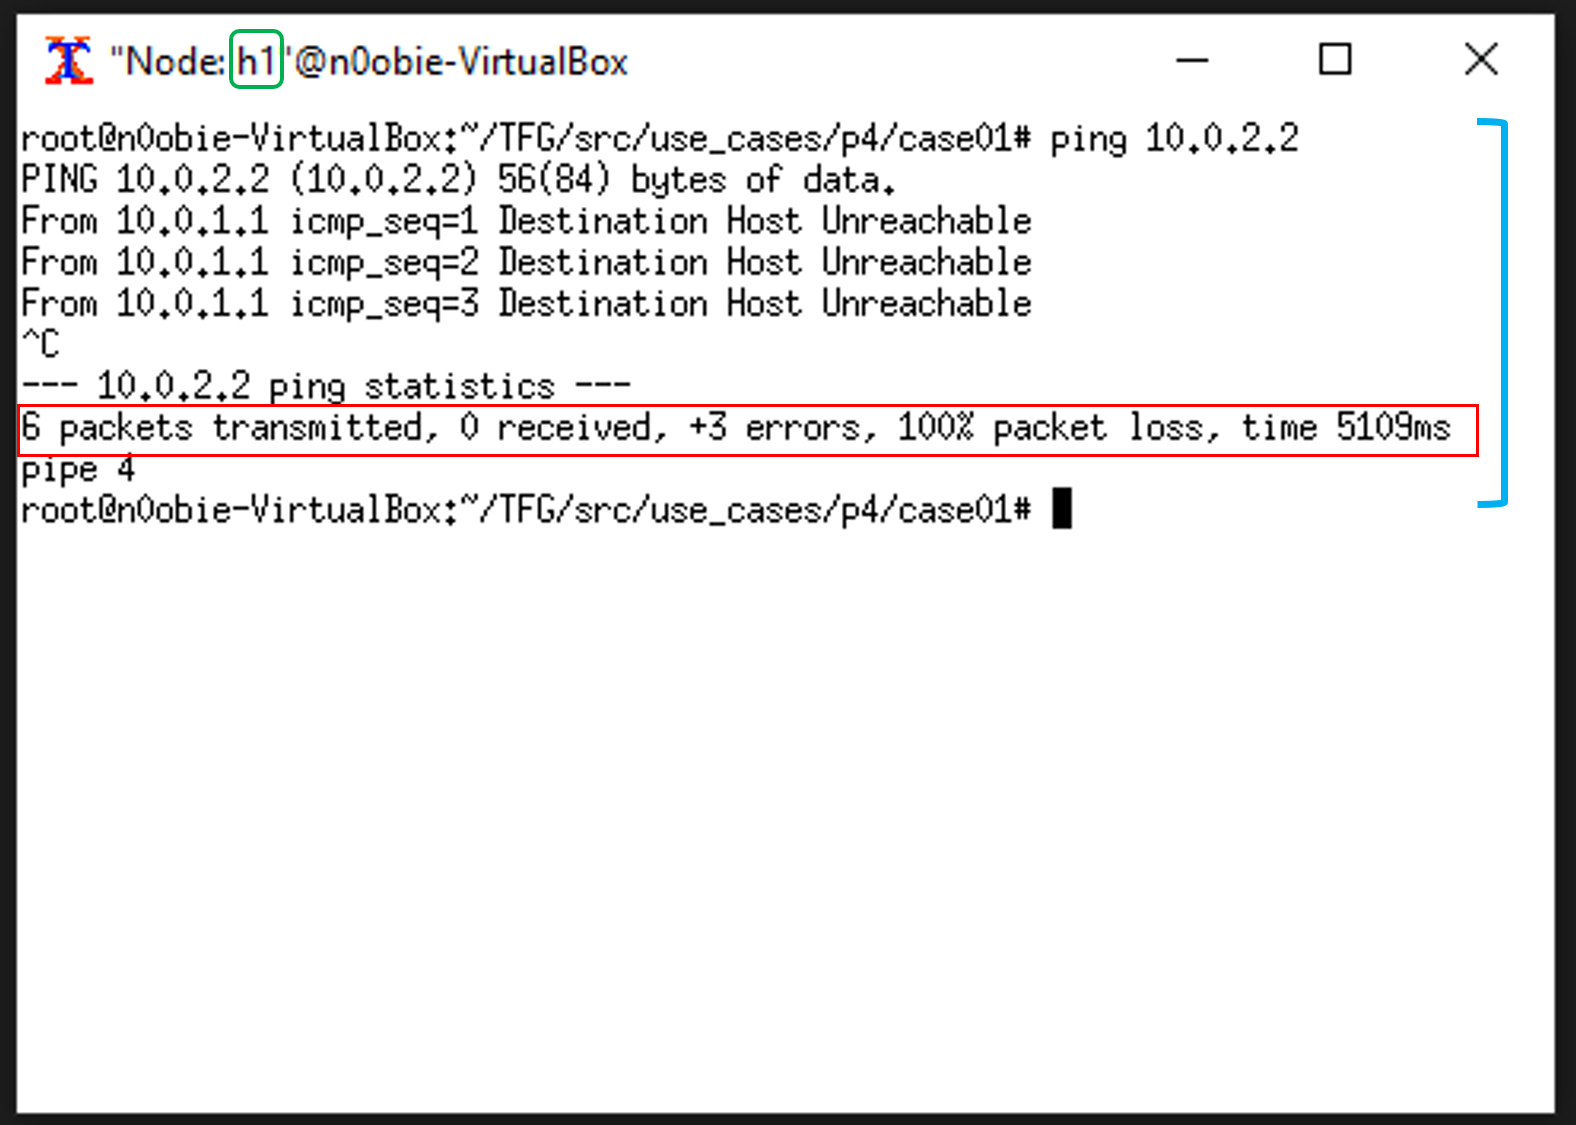
\includegraphics[width=9cm]{archivos/img/dev/p4/case01/demo_case01_1_edited.png}
    \caption{Comprobación de funcionamiento (Ping) del Case01 - P4}
    \label{fig:case01_p4_ether_func1}
\end{figure}
\newpage
\begin{figure}[ht]
    \centering
    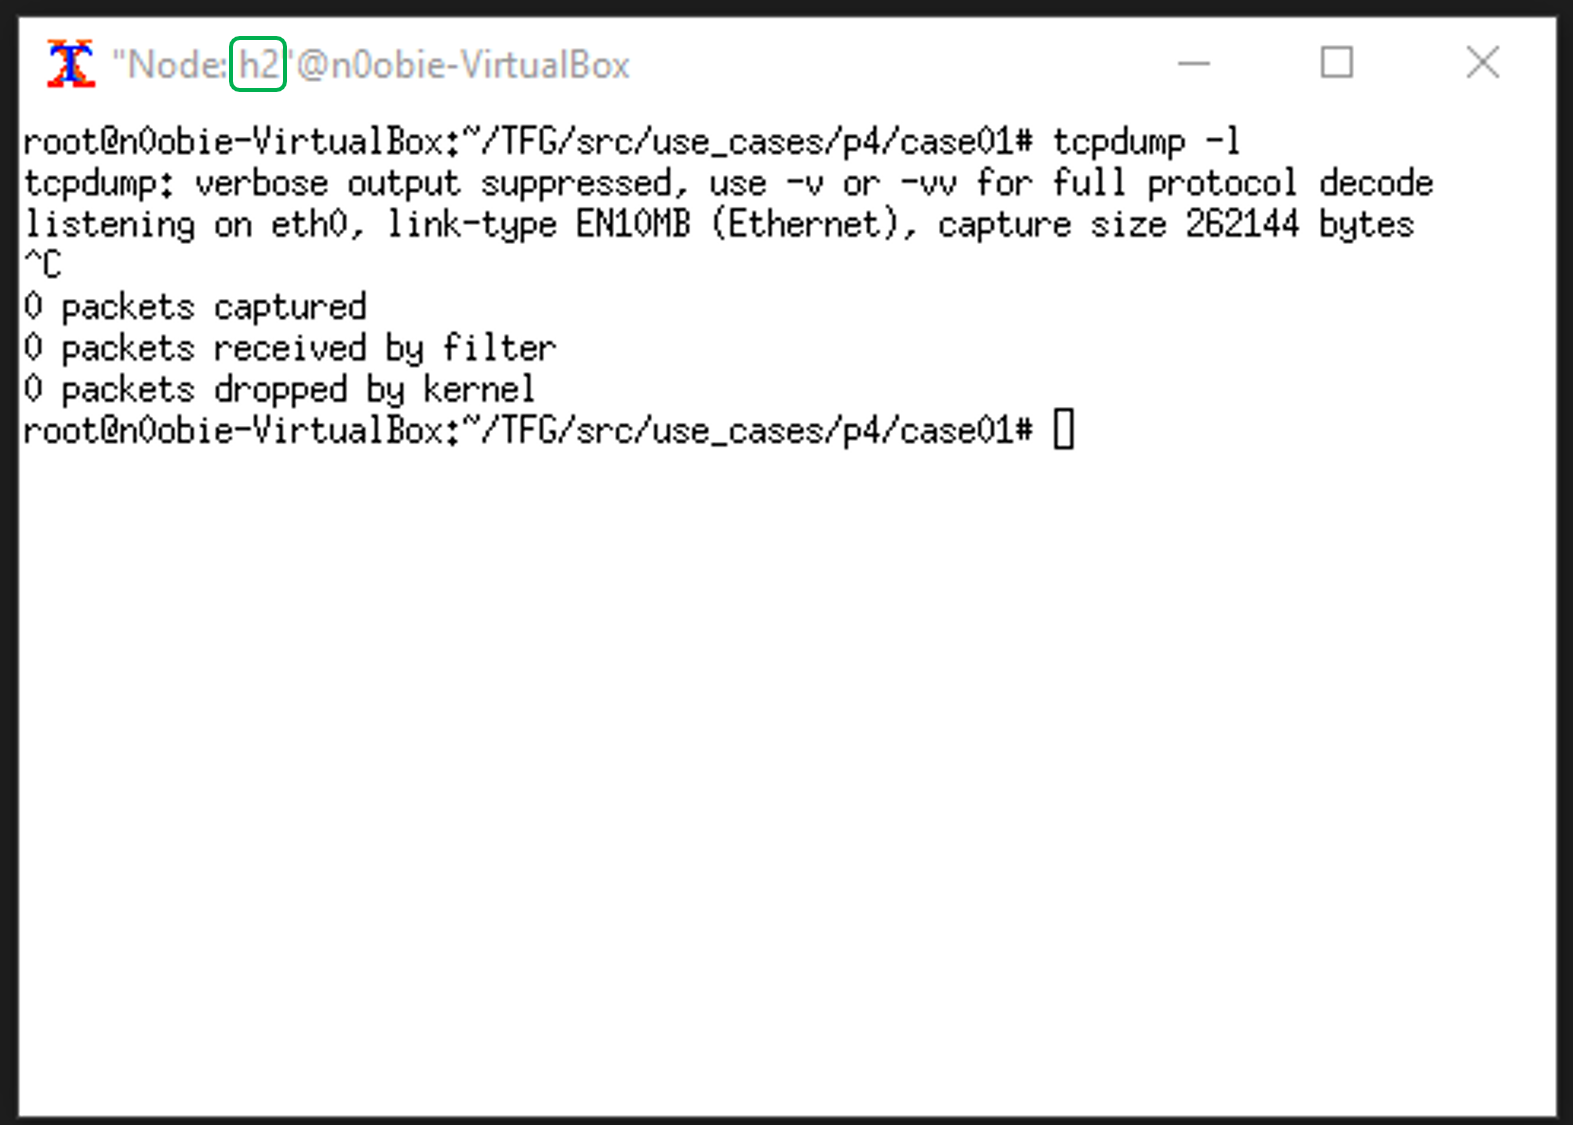
\includegraphics[width=11cm]{archivos/img/dev/p4/case01/demo_case01_2_edited.png}
    \caption{Comprobación de funcionamiento (Sniffer) del Case01 - P4}
    \label{fig:case01_p4_ether_func2}
\end{figure}


Una vez que se esté escuchando en la interfaz del \texttt{host2}, se hará ping \fcolorbox{black}{ProcessBlue}{\rule{0pt}{2.5pt}\rule{2.5pt}{0pt}}\hspace{1mm} desde el \texttt{host1} al \texttt{host2} y no se debería tener conectividad. Como se puede ver en las figuras \ref{fig:case01_p4_ether_func1} y \ref{fig:case01_p4_ether_func2}, el programa P4 desarrollado funciona correctamente. Para asegurarse de que realmente se está ejecutando el action para tirar paquetes se puede consultar los logs del \gls{bmv2}, los cuales generan un fichero de log por cada instancia target del simple switch que se haya levantado. \\
\par
Estos logs se encuentran en el directorio \texttt{logs}, y cada fichero de log pertenece a un único ``switch", llevando el mismo nombre que este en Mininet. En este caso, si se quisieran monitorizar los logs del \texttt{s1} bastaría con seguir las indicaciones del bloque \ref{code:case01_p4_ether_func2}.

\begin{lstlisting}[language= bash, style=Consola, caption={Comprobación de funcionamiento - Case01},label=code:case01_p4_ether_func2]
    # Entramos al directorio 
    cd TFG/src/use_cases/p4/case01

    # Monitorizamos los logs del Switch (s1) 
    tail -f logs/s1.log
\end{lstlisting}
\subsection{Case02 - Pass}
\label{P4_ether_case02}

Como se puede apreciar en esta sección, no se ha desarrollado ningún programa P4. Esto se debe a que no hay equivalente en P4 del código de retorno \texttt{XDP\_PASS}, por ello, no se puede hacer nada en este caso de uso. A continuación, se indica el porqué no se encuentra un equivalente entre ambas tecnologías. El código de de retorno en \gls{xdp} es una forma para llevar a cabo una acción con el paquete que llega a la interfaz, en la cual hay anclado un programa \gls{xdp}. Para más información sobre los códigos de retorno consultar la sección \ref{TecnologiaXDP} donde se indica en detalle cuantos hay, para qué sirven y qué limitaciones tienen.\\
\par

En este caso, el código de retorno \texttt{XDP\_PASS} implica que el paquete se pasa al siguiente punto del procesamiento del \textit{stack} de red en el Kernel de Linux. Es decir, si el programa está anclado a la \gls{nic}, se dejará pasar el paquete al \gls{tc}, de ahí al propio \textit{stack} de red para parsear sus cabeceras, y más adelante, pasárselo a la interfaz de sockets. En P4, el entorno donde se llevarán a cabo los casos de uso será Mininet con ``switches" (\gls{bmv2}) y host. Los ``switches" (\gls{bmv2}) es un soft-switch que permite inyectarle código P4, con el cual se puede definir el \textit{datapath} del mismo.\\
\par

Ahora bien, aquí viene la gran diferencia entre ambas tecnologías, con \gls{xdp} siempre se puede pasar el paquete al Kernel para que se encargue el del procesamiento, pero en P4, se debe definir de forma exclusiva todo el \textit{datapath}, por lo que no hay a quién delegar el paquete, dado que se tiene que encargar el propio programa P4. Entonces, como tal, no habría equivalente del \texttt{XDP\_PASS} en P4.
\subsection{Case03 - Echo server}
\label{P4_ether_case03}


En este caso de uso desarrollaremos un servidor de Echo que responda todos los pings que le lleguen. Como tal el programa P4 no es suficiente para probar esta funcionalidad, como ya se mencionó, se requiere de una plataforma que sea capaz de soportar el lenguaje P4, el \gls{bmv2}. \\
\par

El programa P4 deberá ser capaz de analizar los paquetes que le lleguen, analizarlos y filtrarlos. Solo aquellos paquetes filtrados serán los que se deberán responder. ¿Cómo se filtrarán? Se añadirán nuevos estados en el parser que comprueben si las cabeceras ICMP están presentes. Por ello, antes de nada se debe declarar las cabeceras ICMP necesarias para poder así analizar las cabeceras de los paquetes que lleguen.

\begin{lstlisting}[language=C, style=P4-color, caption={Estructura cabecera ICMP - Case03},label=code:case03_p4_ether_prog1]
    header icmp_t {
    	bit<8> type;
    	bit<8> code;
    	bit<16> checksum;
    }
\end{lstlisting}
\vspace{0.5cm}

Como se quería que este programa P4 fuera compatible con direccionamiento IPv6 se han añadido también los equivalentes en ICMPv6 y la cabecera de red de IPv6, ver bloque \ref{code:case03_p4_ether_prog2}.

\begin{lstlisting}[language=C, style=P4-color, caption={Estructura cabeceras IPv6 e ICMPv6  - Case03},label=code:case03_p4_ether_prog2]
    header ipv6_t {
       bit<4> version;
       bit<8> trafficClass;
       bit<20> flowLabel;
       bit<16> payloadLen;
       bit<8> nextHdr;
       bit<8> hopLimit;
       ip6Addr_t srcAddr;
       ip6Addr_t dstAddr;	
    }
    
    
    header icmp6_t {
       bit<8> type;
       bit<8> code;
       bit<16> checksum;
    }
\end{lstlisting}
\vspace{0.5cm}

Ahora que ya se tiene las cabeceras definidas, se deberá preocuparse en definir las macros asociadas a los posibles \textit{ethertypes} que se quieran manejar, IPv4 y IPv6. De forma adicional, se deberán definir los códigos de protocolo de las cabeceras de red, para asegurare que sobre la cabecera de red únicamente se procesarán aquellos paquetes que porten información ICMP. Se tuvo que consultar la RFC asociada a IPv6 para saber que codificación hacían con el campo de \textit{nextHeader} y por lo visto utilizan los mismo valores que en IPv4. A continuación, en la figura \ref{code:case03_p4_ether_prog3} se puede ver la definición de dichas macros y el extracto de la RFC asociada a la codificación de las cabeceras IPv6 .\\
\par

\begin{lstlisting}[language=C, style=P4-color, caption={Macros para parsear L2 y L3  - Case03},label=code:case03_p4_ether_prog3]
    /*	---	Layer 2 MACROS	     ---	*/
    const bit<16> ETHERTYPE_IPV4 = 0x0800;
    const bit<16> ETHERTYPE_IPV6 = 0x86dd;
    
    /*	---	Layer 3 MACROS	     ---	*/
    const bit<8> IP_PROTOCOL_ICMP = 0x01;
    const bit<8> IP_PROTOCOL_ICMPv6 = 0x3a; 
    const bit<8> ICMP_ECHO_REQUEST_TYPE = 0x08;
    const bit<8> ICMP_ECHO_REQUEST_CODE = 0x00;
    const bit<8> ICMP_ECHO_REPLY_TYPE = 0x00;
    const bit<8> ICMP_ECHO_REPLY_CODE = 0x00;
    
    /*
    *   According to RFC 2460, the codes of the protocol immediately above,
    *   layer 4, are the same as those used in IPv4. And I quote:
    *
    *   Next Header          8-bit selector.  Identifies the type of header
    *                       immediately following the IPv6 header.  Uses the
    *                       same values as the IPv4 Protocol field [RFC-1700
    *                       et seq.].
    *
    */
\end{lstlisting}
\vspace{0.5cm}

Como se ha indicado en el bloque \ref{code:case03_p4_ether_prog3},  de forma adicional se han definido macros sobre los valores con los que se va estar trabajando (\texttt{ECHO-Request} y \texttt{ECHO-Reply}). De esta forma el código resultante de las \textit{actions} será más interpretable y sostenible. Teniendo ya todas las herramientas necesarias para declarar los nuevos estados del parser, se puede proceder con el siguiente bloque del datapath.\\
\par

Una vez que se es capaz de filtrar los paquetes que interesan, se va a ver cómo se ha implementado la lógica de procesamiento de aquellos paquetes que ya han sido filtrados. Es de interés interceptar todos los paquetes ICMP que lleguen a nuestro ``switch" para así contestarlos desde el mismo "switch". Por ello, se hará uso del bit de validez de las cabeceras que han sido analizadas correctamente, es decir, si el paquete contiene dichas cabeceras. De no contenerlas, su bit de validez estará a \textit{false}. A continuación en la figura \ref{code:case03_P4_ether_prog4}, mostramos la lógica de control del bloque \textit{Ingress}.


\begin{lstlisting}[language=C, style=P4-color, caption={Lógica para filtrar paquetes ICMP e ICMPv6  - Case03},label=code:case03_P4_ether_prog4]
    /*  
     *  De esta forma nos aseguramos que unicamente procesamos paquetes ICMP,
     *  o en su defecto ICMPv6.
     *
     */
    
    
    apply {
    	if(hdr.ipv4.isValid() && hdr.icmp.isValid()){
    	        echo();
    	}else if (hdr.ipv6.isValid() && hdr.icmp6.isValid()){
    		echo6();
    	}
    }
\end{lstlisting}
\vspace{0.5cm}

Ya se tienen todos los paquetes ICMP filtrados, solo quedaría programar la lógica para modificar las cabeceras de dicho paquete para conseguir contestar satisfactoriamente al emisor del ping. Para ello, se hará uso de un \textit{action}, una función. El cual intercambiará tanto MAC destino-origen, como IP destino-origen, modificará la cabecera ICMP para indicarle que se trata de un \textit{reply}, y por último mandará el paquete por el puerto por el cual llegó al \gls{bmv2}, de esta forma se asegura que dicho paquete llegará al emisor del mismo.\\
\par


\begin{lstlisting}[language=C, style=P4-color, caption={Lógica para procesar paquetes ICMP  - Case03},label=code:case03_p4_ether_prog5]
    action echo (){
    	/*	---	Auxiliary variables	---	*/
        macAddr_t temp_mac = hdr.ethernet.srcAddr;
        ip4Addr_t temp_ip = hdr.ipv4.srcAddr;
    
    	/*      ---     Swap MACs     ---     */
    	hdr.ethernet.srcAddr = hdr.ethernet.dstAddr;
        hdr.ethernet.dstAddr = temp_mac;
    
    	/*      ---     Swap Ips     ---     */
     	hdr.ipv4.srcAddr = hdr.ipv4.dstAddr;
    	hdr.ipv4.dstAddr = temp_ip;
      
    	/*      ---     Re-Write ICMP's type and code     ---     */
    	hdr.icmp.type = ICMP_ECHO_REPLY_TYPE;
    	hdr.icmp.code = ICMP_ECHO_REPLY_CODE;
    
    	/*      ---     Forward the packet to the ingress intf     ---     */
    	standard_metadata.egress_spec = standard_metadata.ingress_port;

    }  
\end{lstlisting}
\vspace{0.5cm}

\newpage

Préstese atención a la última sentencia de la función donde le indicamos que saque el paquete por la misma interfaz por la cual ha entrado. Este es el equivalente directo al código de retorno en \gls{xdp}, \texttt{XDP\_TX} con el cual re-circulábamos el paquete de la misma forma a la interfaz de entrada.\\
\par

Como curiosidad, es interesante comentar que el campo \textit{checksum} de la cabecera ICMP debe ser re-calculado de nuevo por lo que se deberá hacer antes del \textit{Egress}. Esto supuso un problema, ya que continuamente estaban saliendo paquetes con un \textit{checksum} incorrecto,  lo cual se comprobó con el disector de Wireshark. Finalmente se vio que no había que incluir el campo \textit{checksum} en la nueva suma del nuevo \textit{checksum}\footnote{Habría sido genial que la RFC asociada hubiera estado más clara al respecto.}, de esta forma los paquetes \texttt{ECHO-Reply} que salían ya llevaban el \textit{checksum} calculado correctamente.\\
\par


\vspace{1cm}
\textbf{Compilación y puesta en marcha del escenario}\\
\par

Para la compilación del programa P4 se hará uso de nuevo del compilador P4c (más información sobre el proceso de compilación en la subsección \ref{p4_ether_case01}).\\
\par

Dado que las personas que quieran replicar los casos de uso puede que no estén muy familiarizadas con todo este proceso de compilación y carga en los procesos de \gls{bmv2}, se ha dispuesto un de un Makefile para automatizar las tareas de compilación y carga, y las tareas de limpieza del caso de uso. Para la puesta en marcha del caso de uso se deben seguir los pasos indicados en el bloque \ref{code:case03_p4_ether_load}.\\
\par

\begin{lstlisting}[language= bash, style=Consola, caption={Compilación programa P4 y puesta en marcha del escenario - Case03},label=code:case03_p4_ether_load]
    # Entramos al directorio 
    cd TFG/src/use_cases/p4/case03

    # Hacemos uso del Makefile
    sudo make run
\end{lstlisting}
\vspace{0.5cm}

Una vez se haya finalizado la comprobación del funcionamiento del caso de uso, se debe hacer uso de otro target (\textit{clean}) del Makefile para limpieza total del directorio según se indica en el bloque \ref{code:case03_p4_ether_unload}.

\begin{lstlisting}[language= bash, style=Consola, caption={Limpieza del escenario P4 - Case03},label=code:case03_p4_ether_unload]
    # Hacemos uso del Makefile
    sudo make clean
\end{lstlisting}
\vspace{0.5cm}

Es importante señalar que este target limpiará tanto los ficheros auxiliares para la carga del programa P4 en el \gls{bmv2}, como los directorios de \texttt{pcaps}, \texttt{log}, y \texttt{build} generados en la puesta en marcha del escenario. Por lo que si se desea conservar las capturas de las distintas interfaces de los distintos \gls{bmv2}, se deben copiar o limpiar del escenario a mano siguiendo las indicaciones del bloque \ref{code:case03_p4_ether_unload2}.\\
\par

\begin{lstlisting}[language= bash, style=Consola, caption={Limpieza segura del escenario P4 - Case03},label=code:case03_p4_ether_unload2]
    # Limpiamos Mininet
    sudo mn -c
    
    # Limpiamos los directorios generados dinámicamente en la carga del escenario
    sudo rm -rf build logs
\end{lstlisting}


\vspace{1cm}
\textbf{Comprobación del funcionamiento}\\
\par

Una vez realizado el make run en este directorio, se tendrá levantada la topología descrita para este caso de uso, la cual se puede apreciar en la figura \ref{fig:case03_p4_ether_scenario}. Como en el \textit{datapath} no se contempla el manejo del protocolo ARP, se ha añadido el ARP entry a directamente en los hosts, desde el fichero \texttt{topology.json} consiguiendo así que no se genere la resolución ARP en el envío de los \texttt{ECHO-Request}. En este caso, la demostración se va hacer uso de IPv4, en el caso de querer hacerla con IPv6, se deberá añadir la entrada analoga para el protocolo ND  (\textit{Neighbor Discovery}).\\
\par
% figura escenario
\begin{figure}[ht]
    \centering
    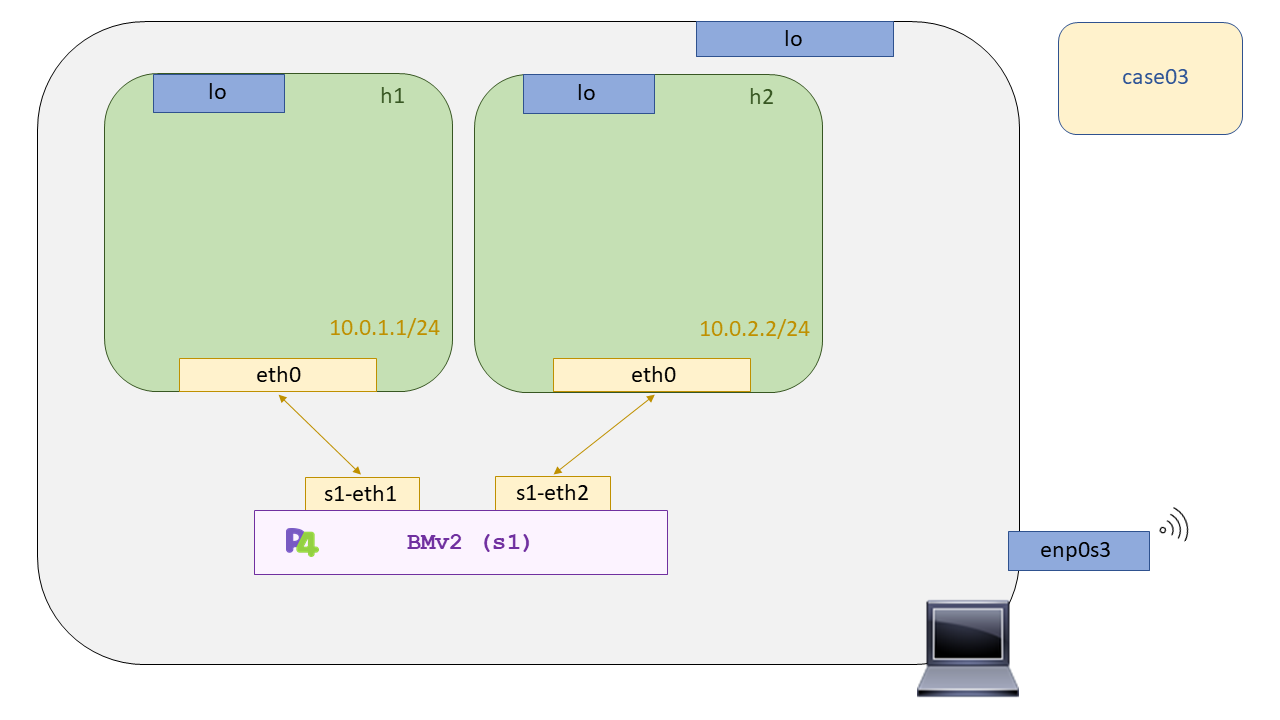
\includegraphics[width=16cm]{archivos/img/dev/p4/case03/scenario.png}
    \caption{Escenario del Case03 - P4}
    \label{fig:case03_p4_ether_scenario}
\end{figure}

Volviendo de nuevo a la comprobación del funcionamiento del caso de uso, se tendrá la CLI de Mininet abierta, por lo que se procederá a abrir una terminal para el \texttt{host1}, desde el cual se llevará a cabo los pings.

\begin{lstlisting}[language= bash, style=Consola, caption={Comprobación de funcionamiento - Case03},label=code:case03_p4_ether_func]
    mininet>  xterm h1
\end{lstlisting}
\vspace{0.5cm}

Una vez que se tenga la terminal abierta, se procederá a abrir Wireshark. En este caso se recomineda Wireshark ya que se podrá filtrar y comprobar de una forma más sencilla la validez de los \textit{checksums}.

% figura escenario
\begin{figure}[ht]
    \centering
    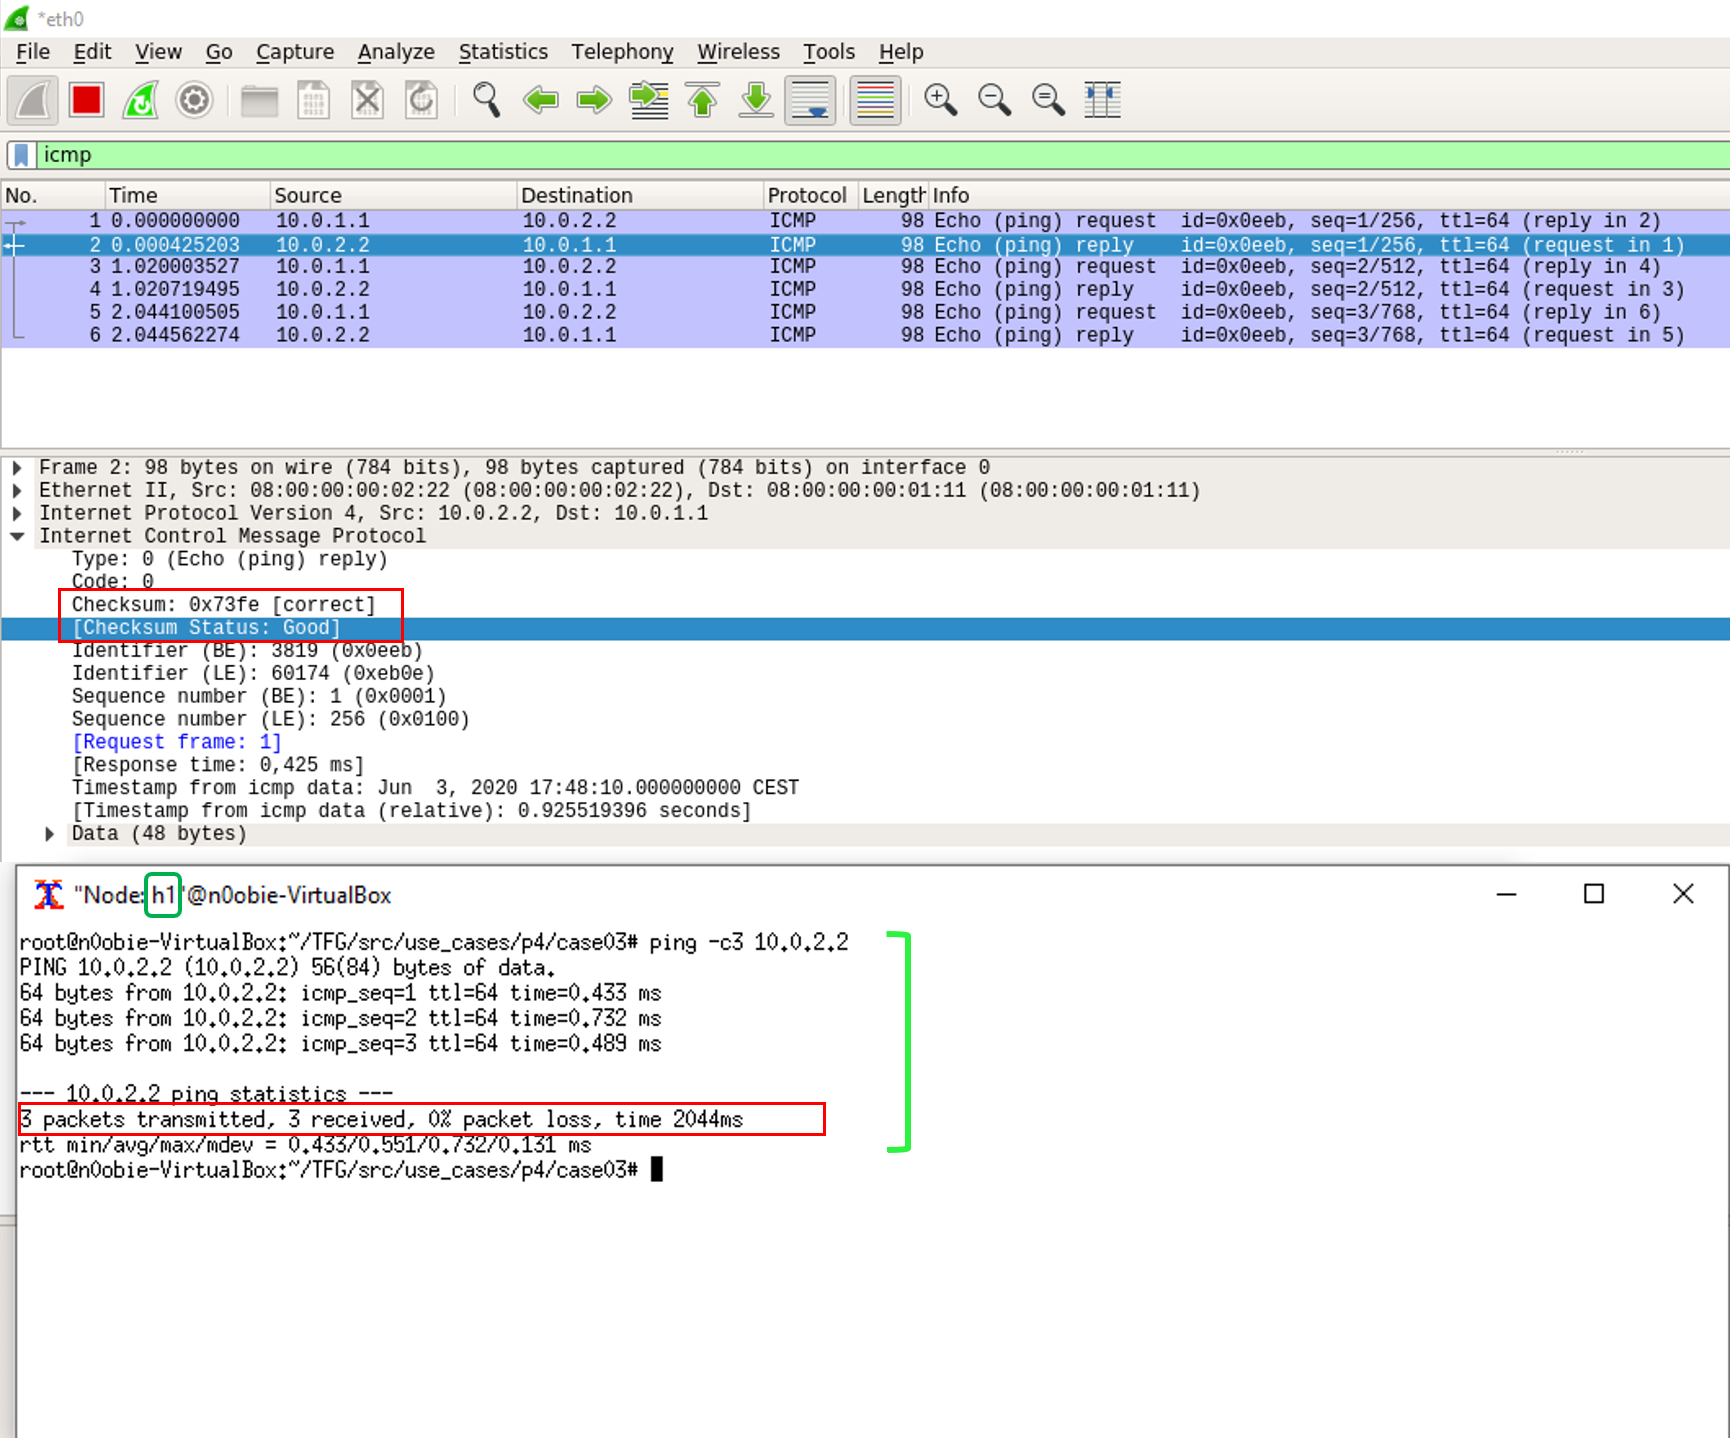
\includegraphics[width=15.5cm]{archivos/img/dev/p4/case03/demo_case03_edited.png}
    \caption{Comprobación de funcionamiento del Case03 - P4}
    \label{fig:case03_p4_ether_func1}
\end{figure}

Como se puede ver en la figura \ref{fig:case03_p4_ether_func1}, todo funciona correctamente ya que se están recibiendo respuesta a los pings \fcolorbox{black}{green}{\rule{0pt}{2.5pt}\rule{2.5pt}{0pt}}\hspace{1mm}. De forma adicional, se puede comprobar con Wireshark como el \textit{checksum} de la cabecera ICMP viene correctamente calculado.


\subsection{Case04 - Layer 3 forwarding}
\label{P4_ether_case04}

En este caso de uso, se abordará la implementación un forwarding a nivel de red, capa 3, por lo que el hipotético ``switch" será ahora un un router muy básico y con muy pocas funcionalidades. Por ello conviene recordar las anotaciones que se hicieron sobre el \gls{bmv2} y por qué no debemos definirlo únicamente como un soft-switch, ya que depende del programa P4 que porte para definir su \textit{datapath} y su interfaz con el plano de control.\\
\par

La motivación de este caso de uso, es ver el equivalente en P4 que tiene el código de retorno \gls{xdp} llamado \texttt{XDP\_REDIRECT}. En el anterior caso de uso ya se hacía uso de la información de metadatos para elegir el puerto de salida del paquete. Por lo que podríamos afirmar que este es el equivalente directo al forwarding en \gls{xdp}, solo que aquí en P4 resulta más sencillo ya que únicamente indicamos por número de puerto mientras que \gls{xdp} se debía obtener el \textit{ifindex} de la interfaz a la cual íbamos a hacer el reenvío. Como se puede apreciar en la figura \ref{code:case04_p4_ether_prog1}, unicamente le indicamos el puerto por el cual debe salir el paquete.\\
\par

\begin{lstlisting}[language=C, style=P4-color, caption={Redirección del paquete - Case04},label=code:case04_p4_ether_prog1]
    standard_metadata.egress_spec = port
\end{lstlisting}
\vspace{0.5cm}

Pero, ¿Qué son los números de puerto? ¿Cuando se han establecido estos identificadores? Estos números de puerto se establecen cuando se levanta la instancia del \gls{bmv2}. Se asocia interfaz real con un número identificativo. Serán estos números identificativos los números de puerto de cada ``switch". De esta manera el ``switch" tiene a su alcance todos sus posibles puertos. El levantamiento de las instancias de \gls{bmv2} se llevan a cabo con la carga del script \texttt{run\_exercise.py}. Este a su vez hace uso de la clase \texttt{P4RuntimeSwitch} definida en la interfaz de Python hacia Mininet,  para levantar dicho ``switch" pasándole los parámetros adecuados. Se puede levantar una instancia del \gls{bmv2} siguiendo las indicaciones del bloque \ref{code:case04_p4_ether_instacia}.\\
\par

\begin{lstlisting}[language= bash, style=Consola, caption={Ejecución de instancia del BMv2 - Case04},label=code:case04_p4_ether_instacia]
    sudo simple_switch_grpc --log-console --dump-packet-data 64 \
                        –i 0@veth0 -i 1@veth2 … [--pcap] --no-p4 \
                        --grpc-server-addr 0.0.0.0:50051 --cpu-port 255 \
                        test.json
\end{lstlisting}
\vspace{0.5cm}
Una vez entendido de dónde salen los números de puerto, se debe plantear la siguiente cuestión, ¿Cómo un programa P4 es capaz de conocer los posibles puertos de los que puede disponer para reenviar un paquete?\\
\par
No puede, y tampoco es lógico que en un programa P4, donde se define el \textit{datapath}, ya estén preestablecidos los números de puerto posibles a manejar. Ya que si eso fuera así, se tendría que tener distintos programas P4 por cada entidad con un número de puertos distintos (únicamente para implementar un único \textit{datapath}). No es viable. Por ello, toda la información relativa a los puertos, asociada al forwarding, generalmente suele venir desde el plano de control quien tiene constancia de los puertos de dicho ``switch".\\
\par

Por ejemplo, si se quiere hacer forwarding de un paquete a un puerto en especifico dado su IP, necesitaremos que el plano de control indique el criterio a seguir, qué IPs están asociadas a según que puertos. Esta interfaz entre el plano de datos y el plano de control esta definidas por tablas.\\
\par

Desde el programa P4 se tiene que definir el esqueleto de la tabla, indicando qué \textit{actions}
están disponibles, qué parámetros reciben esas \textit{actions}, qué criterio de match tendrá la tabla, sobre qué \textit{keys} se realizará el \textit{lookup} y cuál es el número máximo de entradas en dicha tabla. A continuación, se muestra la figura \ref{fig:case03_p4_ether_tablas} que resume bastante bien la funcionalidad de las tablas.\\
\par

% figura escenario
\begin{figure}[ht]
    \centering
    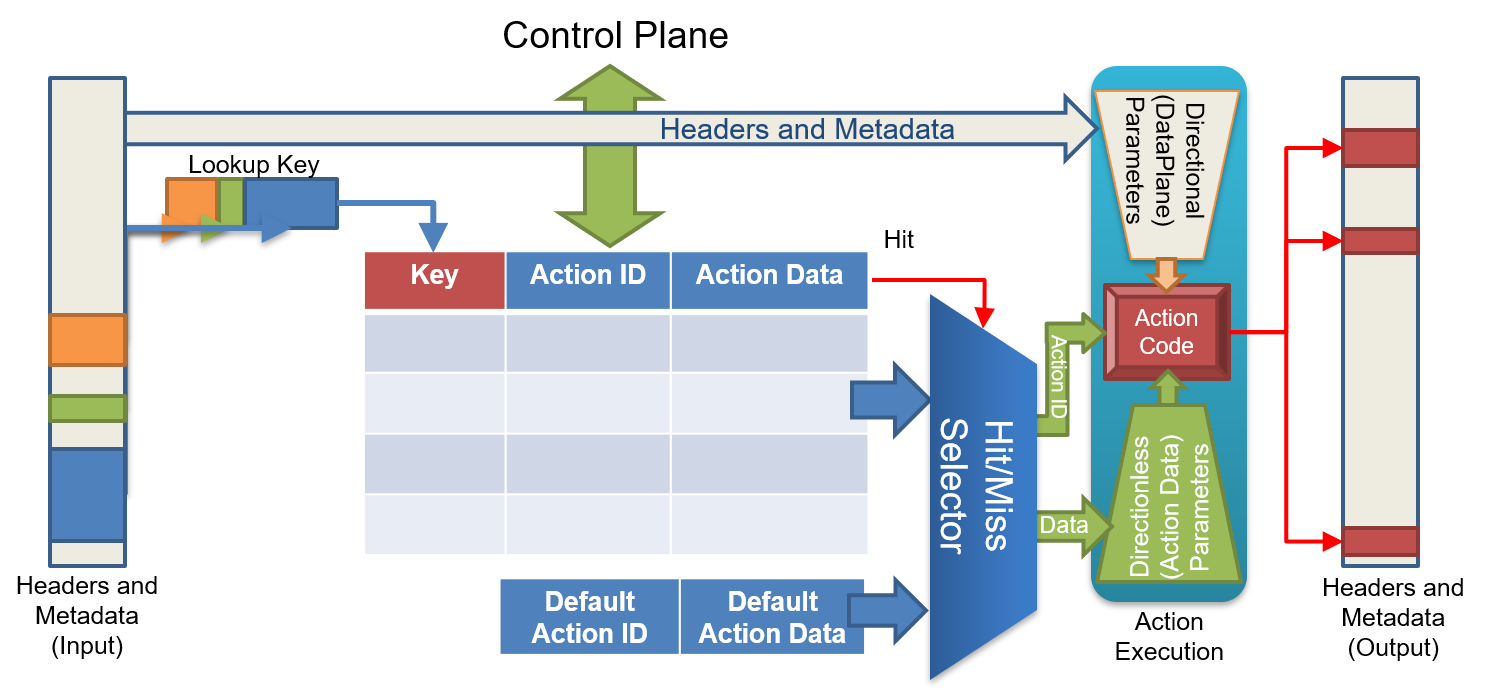
\includegraphics[width=16cm]{archivos/img/dev/p4/case04/table.png}
    \caption{Funcionamiento de las tablas en P4 \cite{p42}}
    \label{fig:case03_p4_ether_tablas}
\end{figure}
\vspace{0.2cm}

Por tanto, desde el plano de control, bien vía P4Runtime ó vía json con los ficheros \texttt{sX-runtime.json} (que se cargarán a través de la CLI-\gls{bmv2}), se rellenarán las entradas de dicha tabla y los parámetros de las acciones a llevar a cabo cuando haya un \textit{hit} con dicha entrada. En este caso se asociarán IPs a una acción de forwarding donde  se le  suministrará por qué puerto tiene que salir el paquete y que MAC destino debe llevar.\\
\par

Una vez entendidos los números de puerto y el concepto de las tablas, se debe abordar el cómo hacer una acción de forwarding para reenviar los paquetes que lleguen al \gls{bmv2}. Esta acción de forwarding deberá se capaz de actualizar el puerto de salida, actualizar la MAC destino y decrementar en uno el campo \texttt{ttl} de la cabecera IP. A continuación, se indica la acción propuesta para llevar a cabo dicho cometido (Ver bloque \ref{code:case04_p4_ether_prog1}).

\begin{lstlisting}[language=C, style=P4-color, caption={Acción propuesta para llevar a cabo el forwarding - Case04},label=code:case04_p4_ether_prog2]
    /*
     * Se quiso hacer uso del operador '-=' pero la sintaxis de P4 no lo permite :(
     */
    
    action ipv4_forward(macAddr_t dstAddr, egressSpec_t port) {
            standard_metadata.egress_spec = port;
            hdr.ethernet.srcAddr = hdr.ethernet.dstAddr;
            hdr.ethernet.dstAddr = dstAddr;
            hdr.ipv4.ttl = hdr.ipv4.ttl - 1;
    }
\end{lstlisting}
\vspace{0.5cm}
Teniendo la acción ya disponible, solo quedaría aplicar la tabla en nuestra pipeline del programa P4 y ya se estaría haciendo un forwarding en capa 3.

\vspace{0.5cm}
\textbf{Compilación y puesta en marcha del escenario}\\
\par

Para la compilación del programa P4 se hará uso del compilador P4c (más información sobre el proceso de compilación en la subsección \ref{p4_ether_case01}).\\
\par

Dado que las personas que quieran replicar los casos de uso puede que no estén muy familiarizadas con todo este proceso de compilación y carga en los procesos de \gls{bmv2}, se ha dispuesto un de un Makefile para automatizar las tareas de compilación y carga, y las tareas de limpieza del caso de uso. Entonces para la puesta en marcha del caso de uso se deben seguir los pasos indicados en el bloque \ref{code:case04_p4_ether_load}.

\begin{lstlisting}[language= bash, style=Consola, caption={Compilación programa P4 y puesta en marcha del escenario - Case04},label=code:case04_p4_ether_load]
    # Entramos al directorio 
    cd TFG/src/use_cases/p4/case04

    # Hacemos uso del Makefile
    sudo make run
\end{lstlisting}
\vspace{0.5cm}

Una vez se haya finalizado la comprobación del funcionamiento del caso de uso, se debe hacer uso de otro target (\textit{clean}) del Makefile para limpieza total del directorio según se indica en el bloque \ref{code:case04_p4_ether_unload}.

\begin{lstlisting}[language= bash, style=Consola, caption={Limpieza del escenario P4 - Case04},label=code:case04_p4_ether_unload]
    # Hacemos uso del Makefile
    sudo make clean
\end{lstlisting}
\vspace{0.5cm}

Es importante señalar que este target limpiará tanto los ficheros auxiliares para la carga del programa P4 en el \gls{bmv2}, como los directorios de \texttt{pcaps}, \texttt{log}, y \texttt{build} generados en la puesta en marcha del escenario. Por lo que si se desea conservar las capturas de las distintas interfaces de los distintos \gls{bmv2}, cópielas o haga la limpieza del escenario a mano siguiendo las indicaciones del bloque \ref{code:case04_p4_ether_unload2}.
\begin{lstlisting}[language= bash, style=Consola, caption={Limpieza segura del escenario P4 - Case04},label=code:case04_p4_ether_unload2]
    # Limpiamos Mininet
    sudo mn -c
    
    # Limpiamos los directorios generados dinámicamente en la carga del escenario
    sudo rm -rf build logs
\end{lstlisting}


\vspace{0.5cm}
\textbf{Comprobación del funcionamiento}\\
\par


Así pues, después de realizar el \texttt{make run} en este directorio, se tendrá levantada la topología descrita para este caso de uso, la cual se puede apreciar en la figura \ref{fig:case04_p4_ether_scenario}. Como en el \textit{datapath} no se contempla el manejo de ARP, se ha añadido el ARP entry a directamente desde el fichero \texttt{topology.json} consiguiendo así que no se genere la resolución ARP en el envío de los \texttt{ECHO-Request}. Este arreglo es poco elegante ya que se le está indicando un hipotético \textit{gateway} que no existe, y se está añadiendo un ARP entry con la MAC de dicho \textit{gateway}. De esta forma, todos los paquetes saldrán con la MAC destino indicada en la entry y no se producirá la resolución ARP. Al llegar al ``switch" el paquete verá modificada su MAC destino en función de su IP destino, por lo que la ``chapuza" no irá a más.\\
\par

% figura escenario
\begin{figure}[ht]
    \centering
    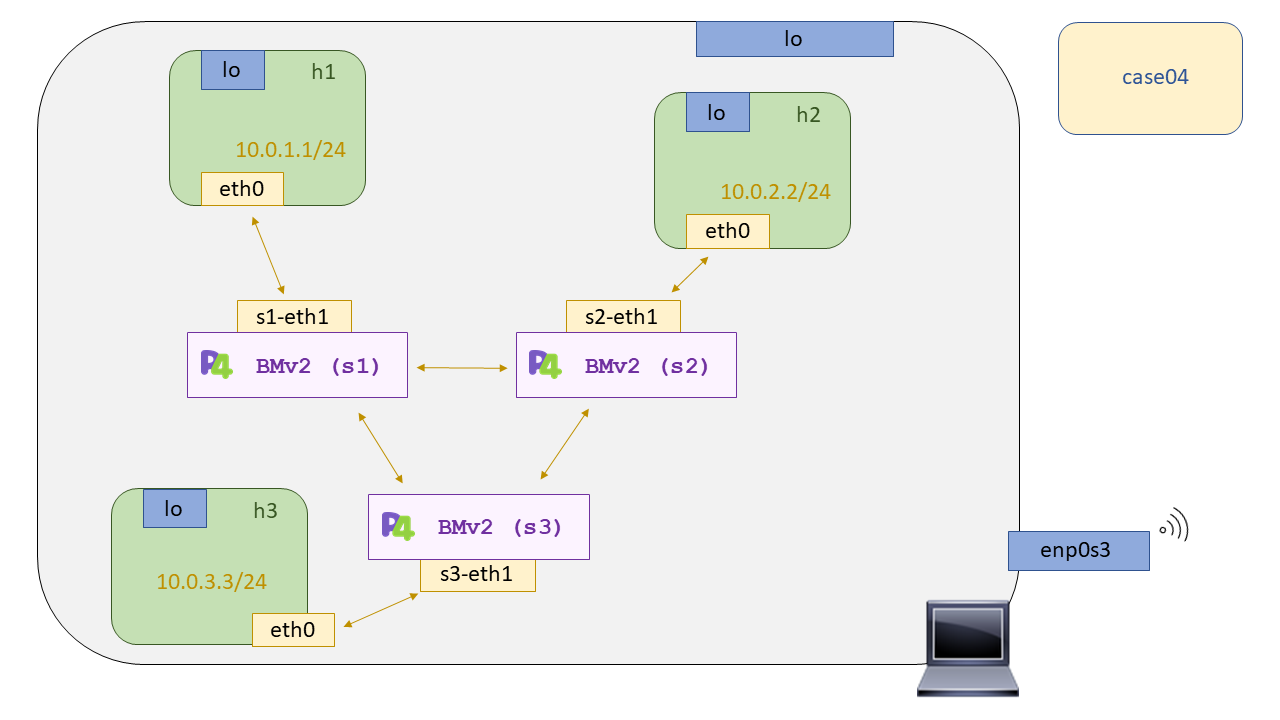
\includegraphics[width=12cm]{archivos/img/dev/p4/case04/scenario.png}
    \caption{Escenario del Case04 - P4}
    \label{fig:case04_p4_ether_scenario}
\end{figure}


Volviendo de nuevo a la comprobación del funcionamiento del caso de uso, se tendrá la CLI de Mininet abierta, por lo que simplemente se probará la conectividad entre todos los hosts. Esto se puede realizar ejecutando la orden \texttt{pingall}, la cual ejecutará pings entre todos los hosts, comprobando así la conectividad bidireccional de todos los \textit{paths} preestablecidos en el escenario. De forma adicional, se podría hacer uso de un \textit{sniffer} para comprobar que los paquetes llegan con el campo \texttt{ttl} modificado, en función de los saltos que ha dado el paquete. Según se puede apreciar en la figura \ref{fig:case04_p4_ether_func}, hay perfecta conectividad entre todos los hosts de la topología.

\newpage

% figura escenario
\begin{figure}[ht]
    \centering
    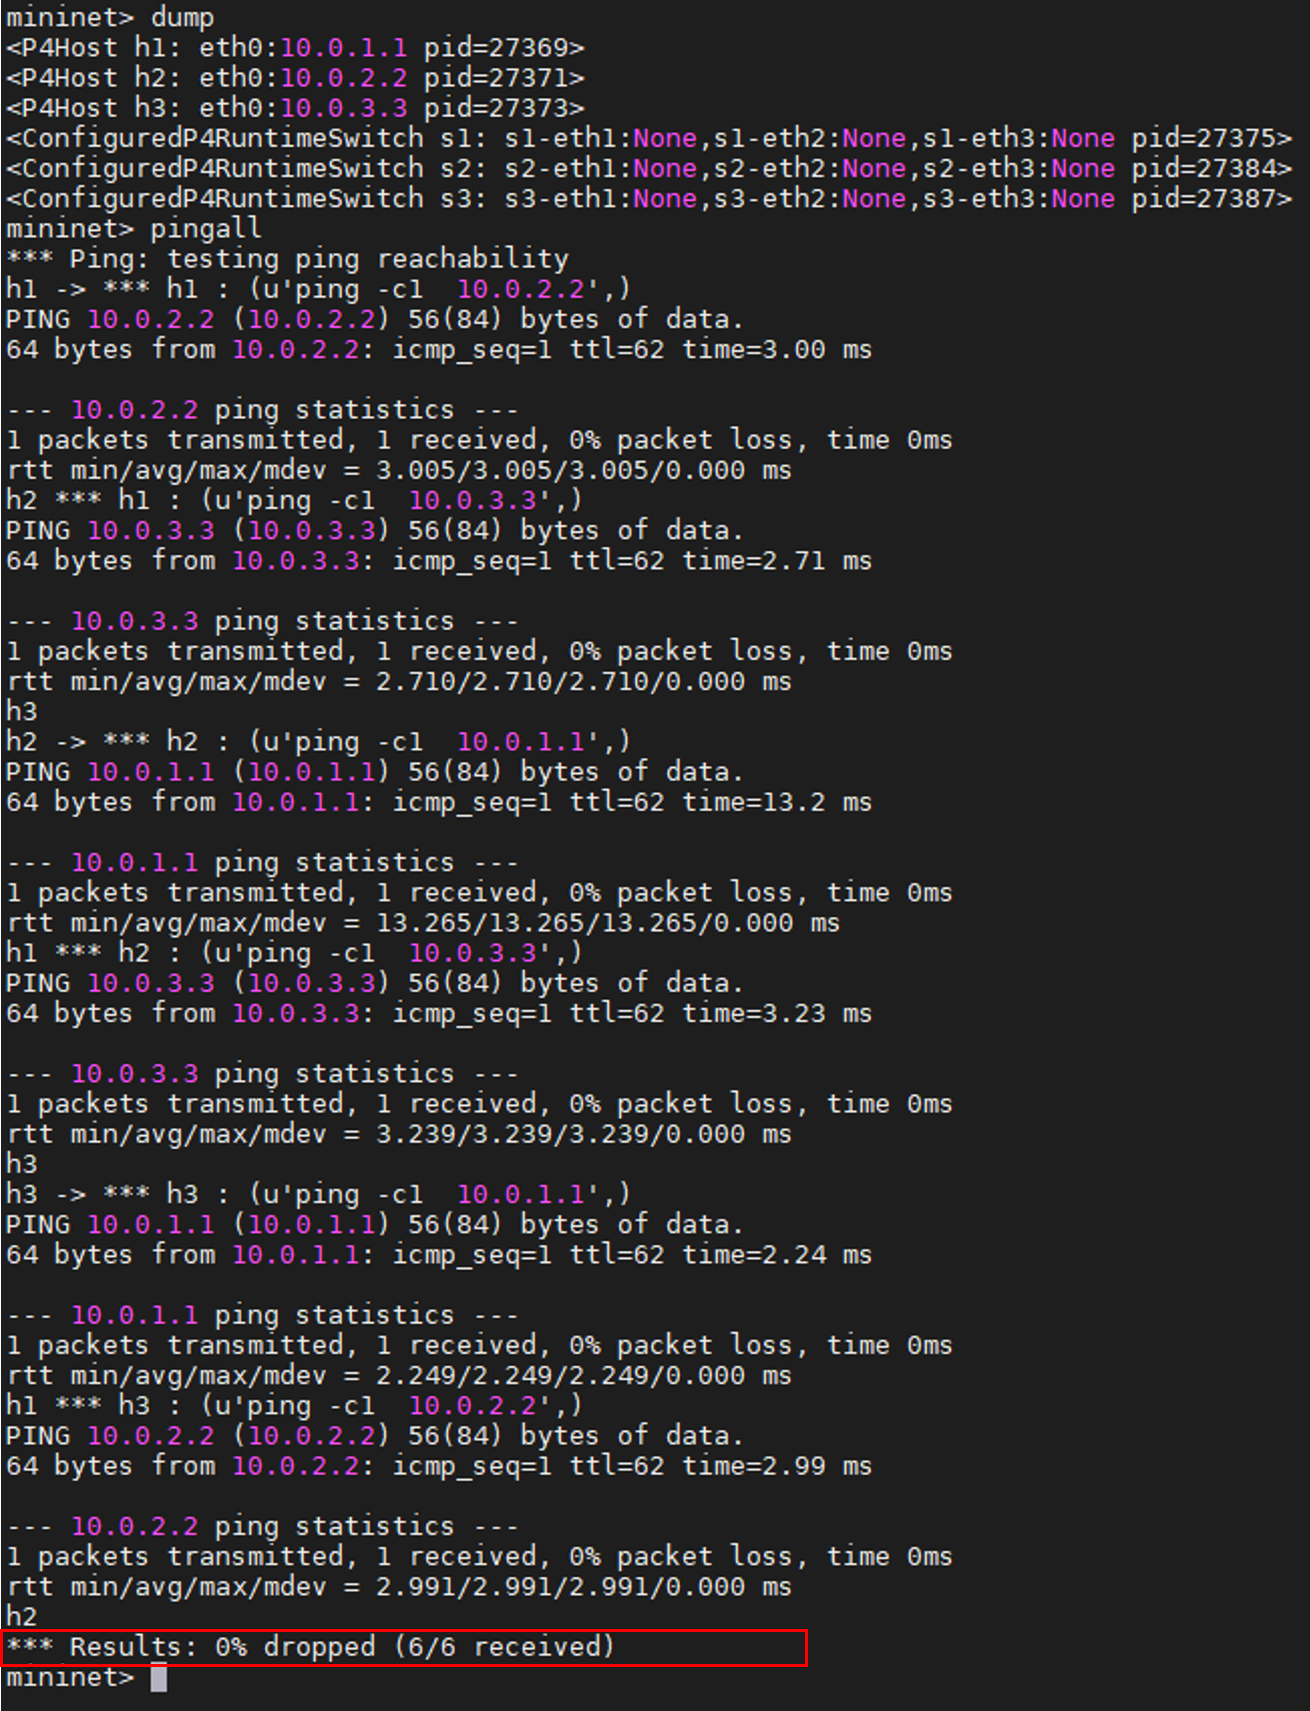
\includegraphics[width=12cm]{archivos/img/dev/p4/case04/demo_case04_edited.png}
    \caption{Comprobación de funcionamiento del Case04 - P4}
    \label{fig:case04_p4_ether_func}
\end{figure}

\newpage


\subsection{Case05 - Broadcast}
\label{P4_ether_case05}

En este caso de uso, se desarrollará un programa p4 que haga Broadcast. En este caso únicamente se hará Broadcast a nivel de enlace, capa 2. La motivación de este caso de uso es ver la diferencia de dificultad respecto del entorno \gls{xdp} donde se tuvo que anclar de manera adicional un \textit{bytecode} e\gls{bpf} en el \gls{tc}, además del propio programa \gls{xdp} anclado en la interfaz para lograr realizar un broadcast.\\
\par

Para conseguir hacer una difusión de los paquetes en P4, se hará uso de los llamados grupos multicast. Los grupos multicast se utilizan para difundir por una serie de números de puertos del ``switch". Para más información sobre de dónde salen estos números de puerto vuelva al case04 (\ref{P4_ether_case04}) donde se explica que representan estos identificadores y cuándo se asignan. Cada grupo multicast tiene un identificador único, y en él se definen una serie de réplicas, es decir, cuántas copias del paquete se llevarán a cabo y qué números de puerto se verán afectados.\\
\par

Los grupos multicast se definen en la información del plano de control del ``switch", bien vía P4Runtime ó vía json con los ficheros \texttt{sX-runtime.json}. A continuación, en el bloque \ref{code:case05_p4_ether_json} se deja la definición del grupo multicast utilizado para este caso de uso.  

\begin{lstlisting}[language= bash, style=Consola, caption={Ejemplo Json Grupo Multicast - Case05},label=code:case05_p4_ether_json]
    "multicast_group_entries" : [
        {
          "multicast_group_id" : 1,
          "replicas" : [
            {
              "egress_port" : 1,
              "instance" : 1
            },
            {
              "egress_port" : 2,
              "instance" : 1
            },
            {
              "egress_port" : 3,
              "instance" : 1
            }
          ]
        }
      ]
\end{lstlisting}
\vspace{0.5cm}

Con esta definición se está indicando que todos los paquetes que pertenezcan al grupo multicast cuyo identificador sea 1, generarán una copia del paquete por los puertos del ``switch" 1, 2 y 3. Es decir por todos los puertos de nuestro ``switch" para este caso de uso. Por tanto la acción de broadcast/multicast será la siguiente:

\begin{lstlisting}[language=C, style=P4-color, caption={Acción propuesta para llevar a cabo el Broadcast - Case05},label=code:case05_p4_ether_prog1]
    action multicast() {
            standard_metadata.mcast_grp = 1;
    }
\end{lstlisting}
\vspace{0.5cm}

Únicamente se asigna el paquete a dicho grupo multicast, y el \gls{bmv2} ya se encarga de clonar el paquete y reenviarlo por los puertos indicados. Dado que no se quiere generar paquetes por el puerto por el cual se recibió el paquete de broadcast, podría plantearse tener tantos grupos multicast como puertos tuviera el \gls{bmv2}, generando copias por puertos específicos y asociando cada grupo multicast a los paquetes que llegaran por cada puerto. Pero esta solución no sería del todo escalable. Por ello, como se puede ver en el grupo multicast (bloque de código \ref{code:case05_p4_ether_json}), se generan copias en todos los puertos asociados a esta instancia del \gls{bmv2}. Será por tanto en la fase de egress cuando se comprueben los metadatos del paquete, y si el puerto de entrada es igual al puerto de salida, se descartará el paquete (Ver bloque de código \ref{code:case05_p4_ether_prog2}).\\
\par

\begin{lstlisting}[language=C, style=P4-color, caption={Acción propuesta para descartar paquetes sobrantes de Broadcast - Case05},label=code:case05_p4_ether_prog2]
    control MyEgress(inout headers hdr,
                 inout metadata meta,
                 inout standard_metadata_t standard_metadata) {
    
        action drop() {
            mark_to_drop(standard_metadata);
        }
    
        apply {
            // Prune multicast packet to ingress port to preventing loop
            if (standard_metadata.egress_port == standard_metadata.ingress_port)
                drop();
        }
}

\end{lstlisting}
\vspace{0.5cm}

En este caso, se ha encontrado que implementar esta funcionalidad en P4 es mucho más sencillo que con \gls{xdp}. Por lo que, en caso de necesitar probar protocolos que implementen la difusión como parte de su lógica, es mucho más recomendable y viable hacer uso de P4.

\vspace{0.5cm}
\textbf{Compilación y puesta en marcha del escenario}\\
\par

Para la compilación del programa P4 se hará uso del compilador P4c (más información sobre el proceso de compilación en la subsección \ref{p4_ether_case01}).\\
\par

Dado que las personas que quieran replicar los casos de uso puede que no estén muy familiarizadas con todo este proceso de compilación y carga en los procesos de \gls{bmv2}, se ha dispuesto un de un Makefile para automatizar las tareas de compilación y carga, y las tareas de limpieza del caso de uso. Entonces para la puesta en marcha del caso de uso se deben seguir los pasos indicados en el bloque \ref{code:case05_p4_ether_load}.

\begin{lstlisting}[language= bash, style=Consola, caption={Compilación programa P4 y puesta en marcha del escenario - Case05},label=code:case05_p4_ether_load]
    # Entramos al directorio 
    cd TFG/src/use_cases/p4/case05

    # Hacemos uso del Makefile
    sudo make run
\end{lstlisting}
\vspace{0.5cm}

Una vez se haya finalizado la comprobación del funcionamiento del caso de uso, se debe hacer uso de otro target (\textit{clean}) del Makefile para limpieza total del directorio según se indica en el bloque \ref{code:case05_p4_ether_unload}.

\begin{lstlisting}[language= bash, style=Consola, caption={Limpieza del escenario P4 - Case05},label=code:case05_p4_ether_unload]
    # Hacemos uso del Makefile
    sudo make clean
\end{lstlisting}
\vspace{0.5cm}

Es importante señalar que este target limpiará tanto los ficheros auxiliares para la carga del programa P4 en el \gls{bmv2}, como los directorios de \texttt{pcaps}, \texttt{log}, y \texttt{build} generados en la puesta en marcha del escenario. Por lo que si se desea conservar las capturas de las distintas interfaces de los distintos \gls{bmv2}, cópielas o haga la limpieza del escenario a mano siguiendo las indicaciones del bloque \ref{code:case05_p4_ether_unload2}.\\
\par

\begin{lstlisting}[language= bash, style=Consola, caption={Limpieza segura del escenario P4 - Case04},label=code:case05_p4_ether_unload2]
    # Limpiamos Mininet
    sudo mn -c
    
    # Limpiamos los directorios generados dinámicamente en la carga del escenario
    sudo rm -rf build logs
\end{lstlisting}


\vspace{0.5cm}
\textbf{Comprobación del funcionamiento}\\
\par
Una vez realizado el make run en el directorio, se tendrá levantada la topología descrita para este caso de uso, la cual se puede apreciar en la figura \ref{fig:case05_p4_ether_scenario}.


% figura escenario
\begin{figure}[ht]
    \centering
    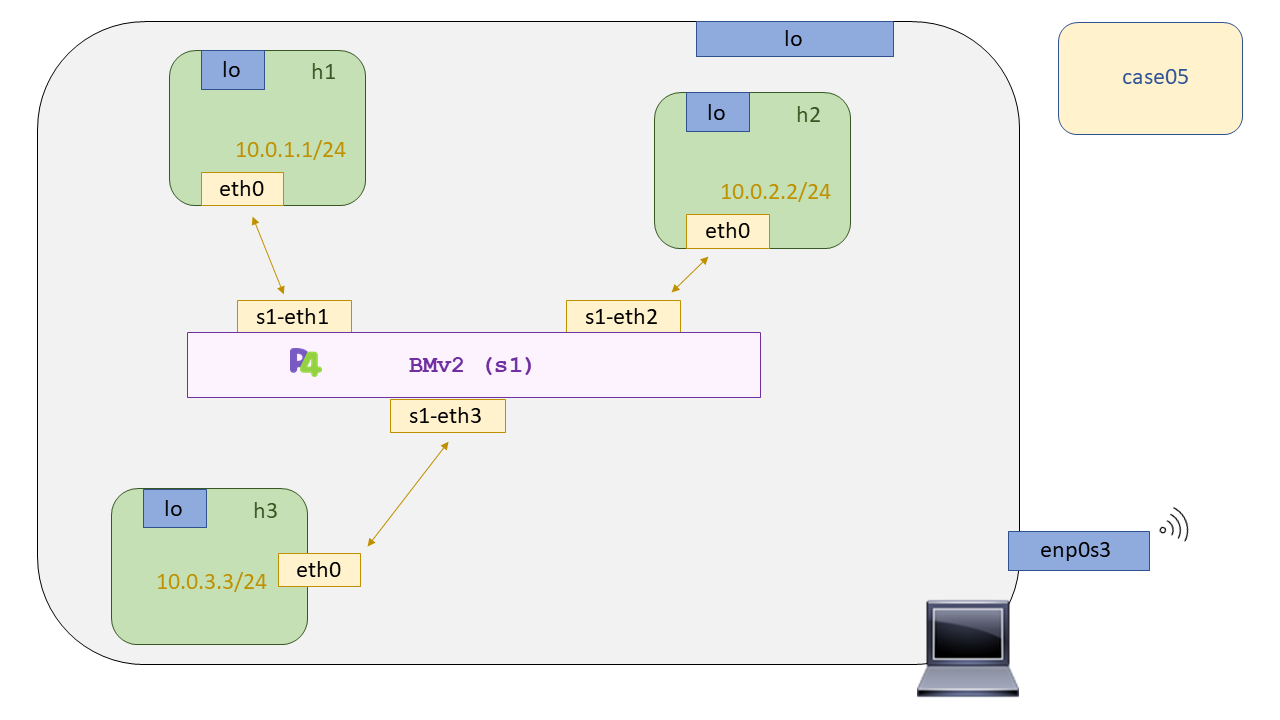
\includegraphics[width=16cm]{archivos/img/dev/p4/case05/scenario.png}
    \caption{Escenario del Case05 - P4}
    \label{fig:case05_p4_ether_scenario}
\end{figure}

Volviendo de nuevo a la comprobación del funcionamiento del caso de uso, se tendrá la CLI de Mininet abierta, por lo que se procederá a abrir tres terminales, una por cada host de la topología. Esto se puede hacer conseguir siguiendo las indicaciones del bloque \ref{code:case05_p4_ether_func1}.

\begin{lstlisting}[language= bash, style=Consola, caption={Apertura de terminales - Case05},label=code:case05_p4_ether_func1]
    mininet> xterm h1 h2 h3 
\end{lstlisting}
\vspace{0.5cm}

Cuando ya se tengan las tres terminales abiertas, se procederá a escuchar las interfaces de los \texttt{host2} y \texttt{host3} con la finalidad de comprobar si realmente los paquetes están siendo clonados por los puertos indicados por el grupo multicast. Se hará uso de la herramienta tcpdump, podríamos utilizar también Wireshark.

\begin{lstlisting}[language= bash, style=Consola, caption={Puesta en escucha - Case05},label=code:case05_p4_ether_func2]
    # Hacemos lo mismo en el host2 y host3
    tcpdump -l
\end{lstlisting}
\vspace{1cm}

Una vez que se tenga tcmdump escuchando desde el \texttt{host2} y \texttt{host3}, se va a generar ARP-Request desde el \texttt{host1} para que así, al ir con MAC destino en difusión se propague por todos los posibles puertos del ``switch" menos por aquel por el cual le llegó. Por tanto, para generar dicho ARP-Request se seguirán los pasos del bloque \ref{code:case05_p4_ether_func3}.

\begin{lstlisting}[language= bash, style=Consola, caption={Generación de ARP-Request - Case05},label=code:case05_p4_ether_func3]
    # Desde el host1
    arping 10.0.2.2
\end{lstlisting}
\vspace{1cm}

Como se puede apreciar en la figura \ref{fig:case05_p4_ether_func1}, el caso de uso funciona correctamente. Se puede observar cómo el paquete ARP-Request está llegando tanto al \texttt{host2} como al \texttt{host3}. Pero solo será el \texttt{host2}, en este caso, el que contesta ya que va dirigido a éste. Se puede ver que al \texttt{host3} solo le llega un ARP-Request, y después se detiene.\\
\par
Esto es así ya que al completarse la resolución ARP el \texttt{host1} ya conoce la dirección MAC del \texttt{host2}, por tanto los ARP-Request que se generen a posteriori llevarán la MAC destino la del \texttt{host2}, entonces el ``switch" no lo difundirá por todos su puertos, se lo pasará directamente al \texttt{host2}.\\
\par

\newpage

\begin{figure}[h!]
    \centering
    \begin{subfigure}[b]{\textwidth}
    	\centering
        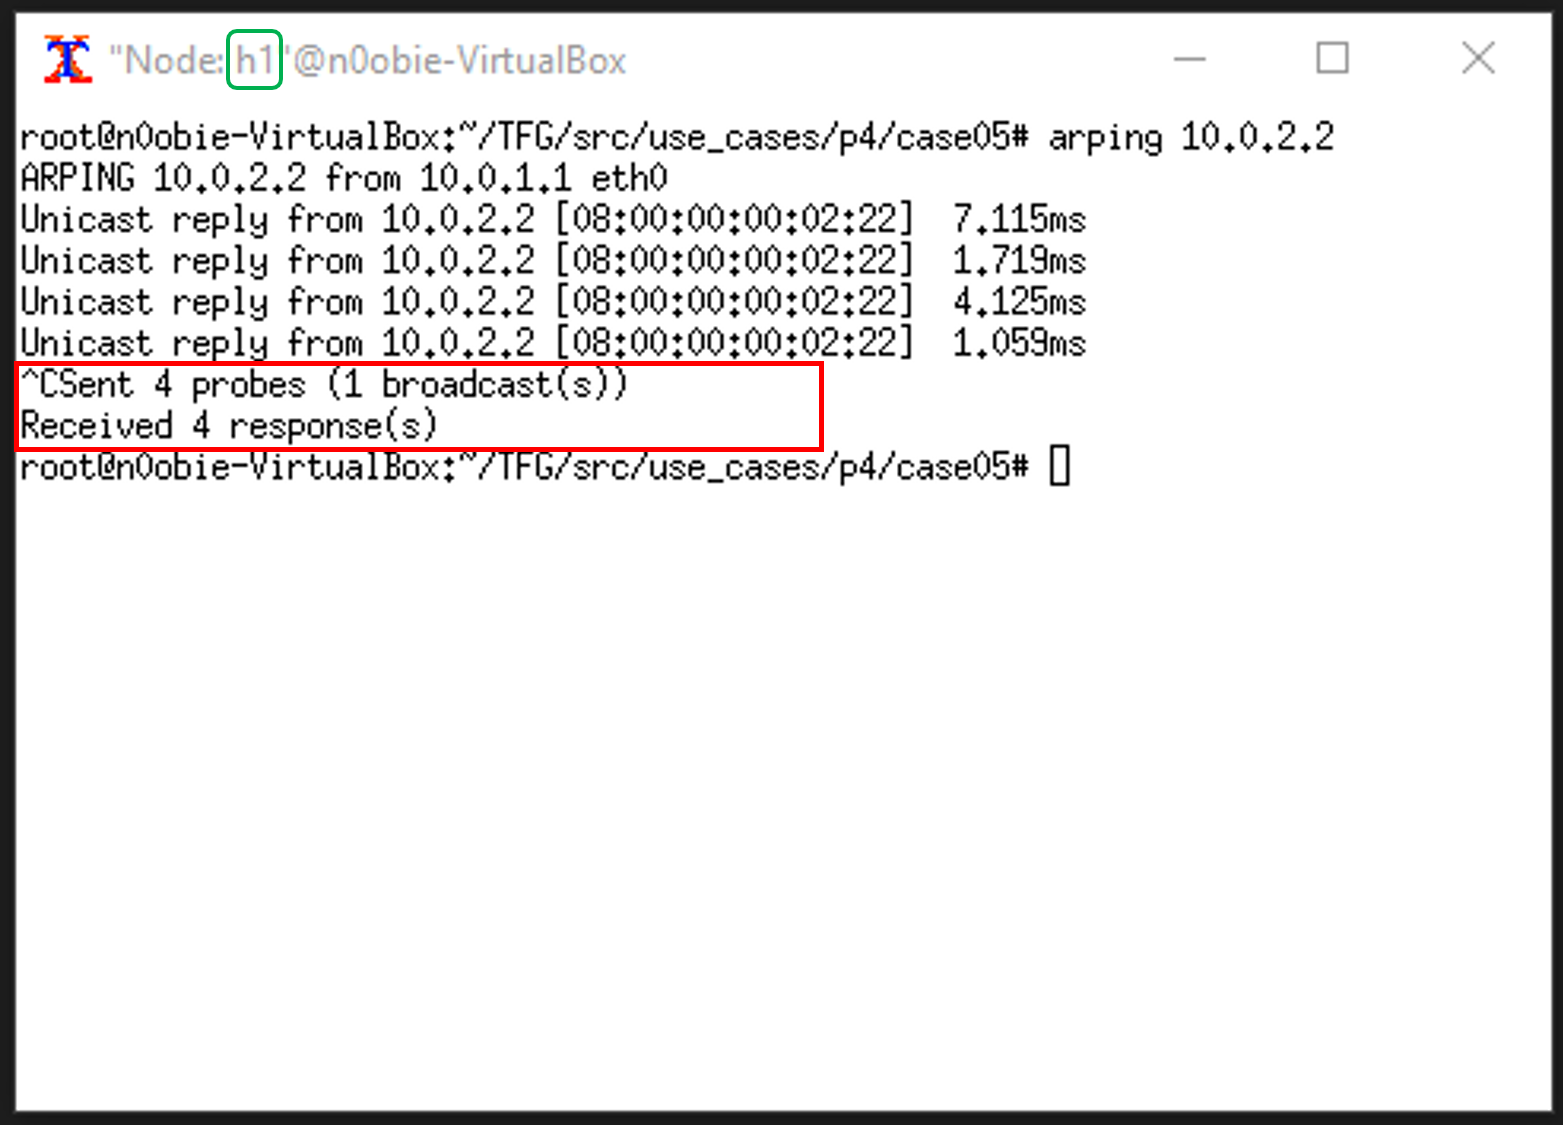
\includegraphics[width=8.2cm]{archivos/img/dev/p4/case05/demo_case05_1_edited.png}
        \caption{Ejecución de arping en el Host1 hacia el Host2}
        \label{fig:case05_p4_ether_func_ping}
    \end{subfigure}
    \par\bigskip
    \begin{subfigure}[b]{\textwidth}
    	\centering
        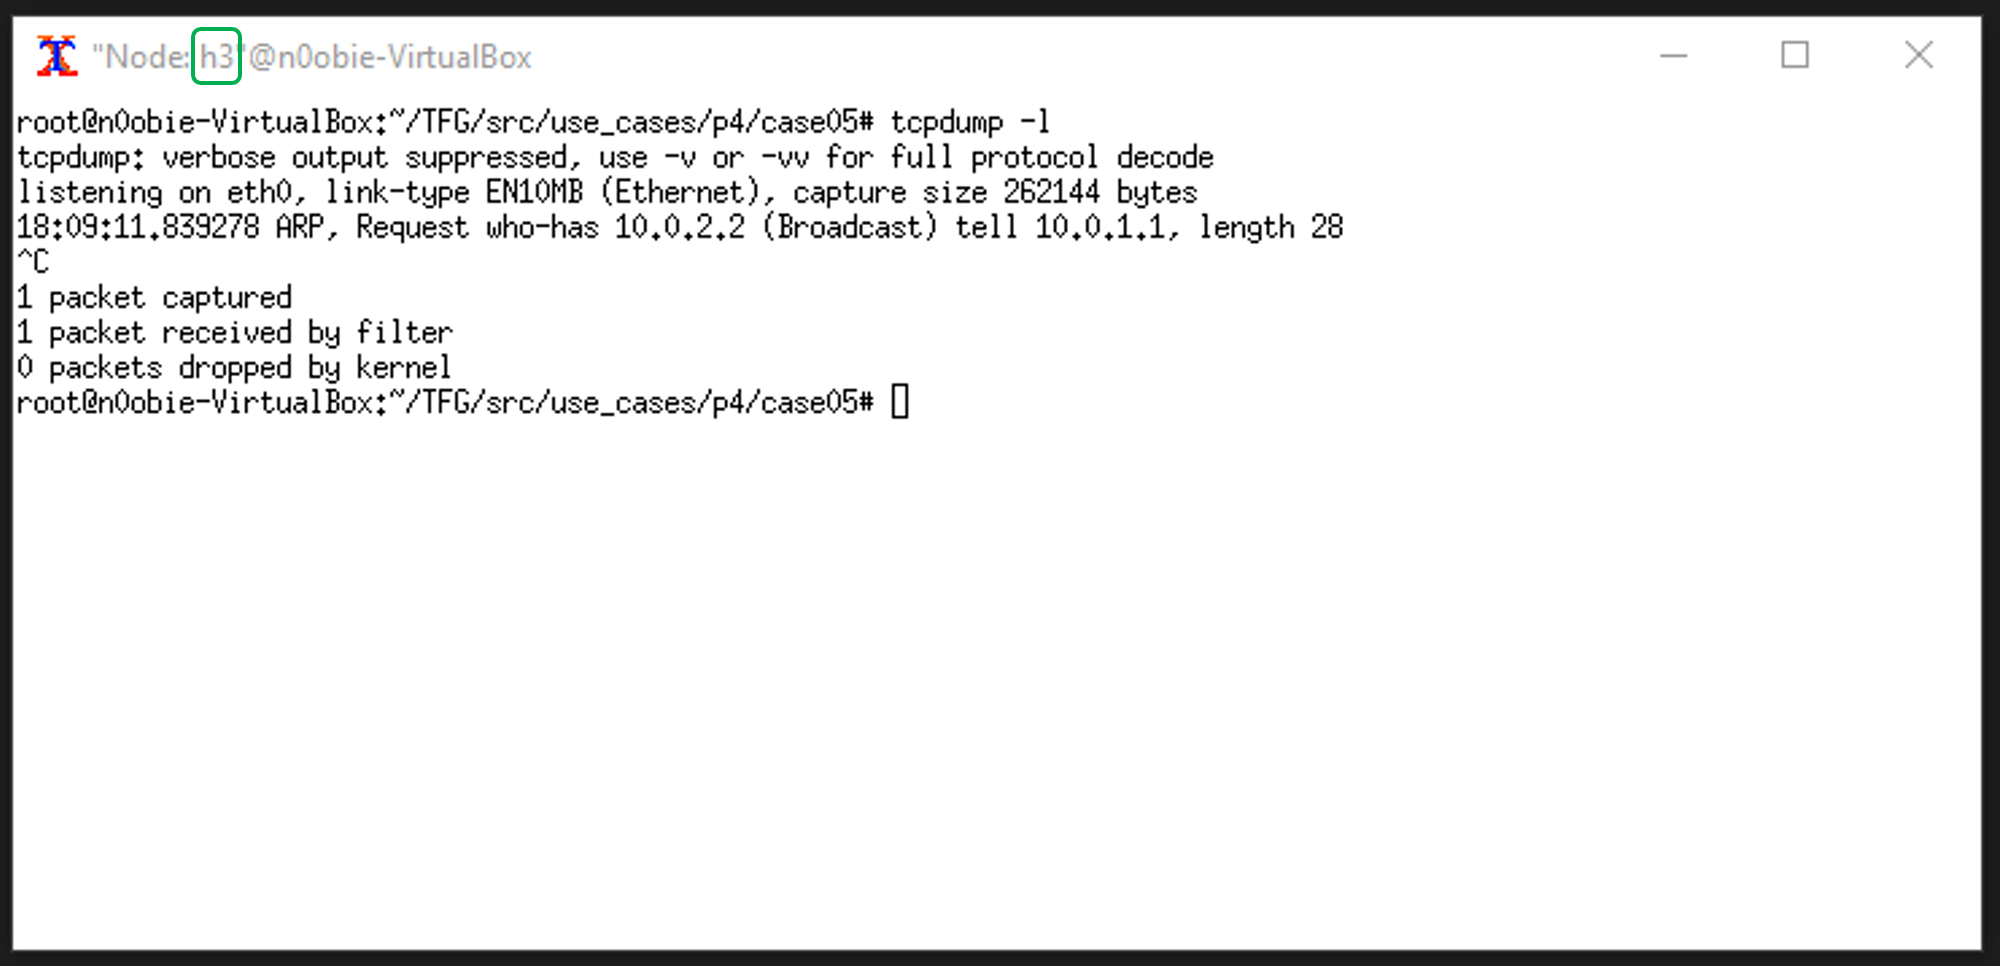
\includegraphics[width=12cm]{archivos/img/dev/p4/case05/demo_case05_2_edited.png}
        \caption{Escucha con Tcpdump en el Host3}
        \label{fig:case05_p4_ether_func_list1}
    \end{subfigure}
    \par\bigskip
    \begin{subfigure}[b]{\textwidth}
    	\centering
        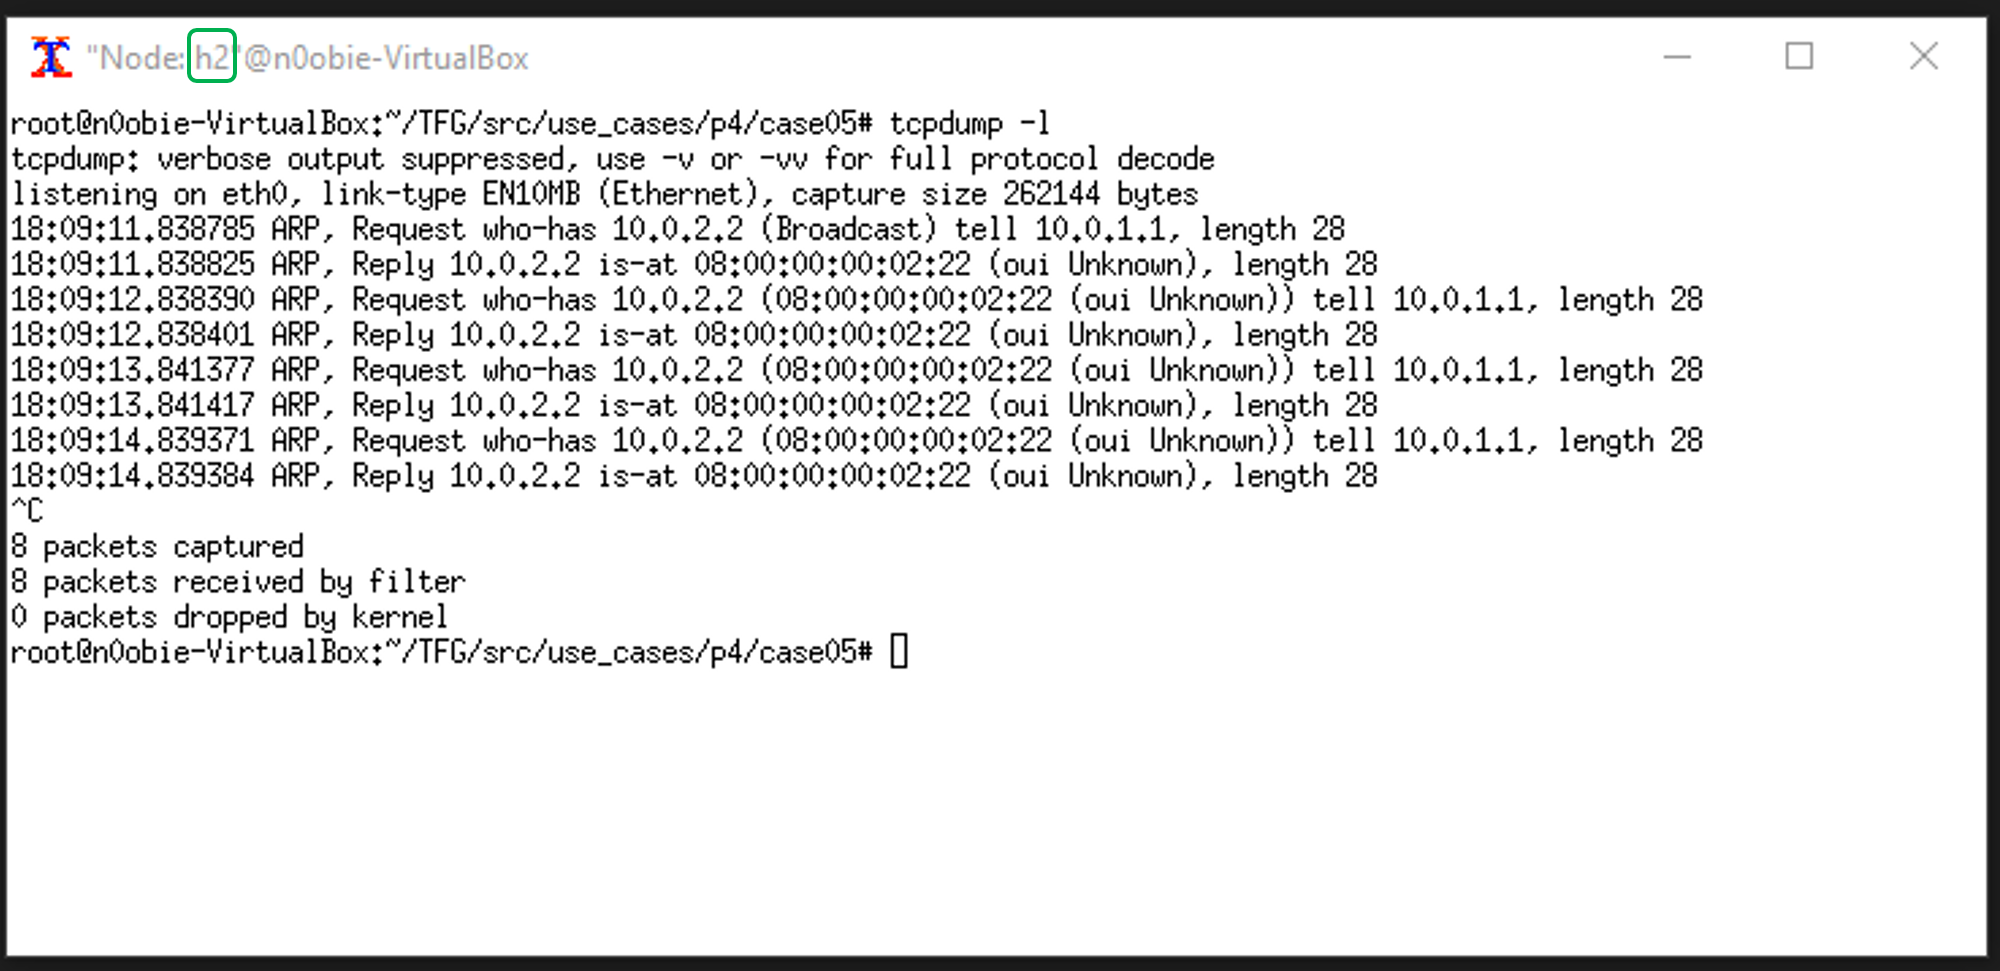
\includegraphics[width=12cm]{archivos/img/dev/p4/case05/demo_case05_3_edited.png}
        \caption{Escucha con Tcpdump en el Host2}
        \label{fig:case05_p4_ether_func_list2}
    \end{subfigure}
    
    \caption{Comprobación de funcionamiento del Case05 - P4}
    \label{fig:case05_p4_ether_func1}
\end{figure}

\newpage


%%%%%%%%%%%%%%%%%%%%%%%%%%%%%%%%%%%%%%%%%%%%%%%%%%%%%%%%%%%%%%%%%%%%%%%%%%%%%%%%%%%%%%%%

\section{Casos de uso P4 en medios inalámbricos}

En esta sección se introducirán todos los casos de uso realizados con la tecnología P4 en entornos inalámbricos. Todos ellos se han nombrado siguiendo la misma sintaxis que en el repositorio del \gls{tfg}, alojado en GitHub. Para \textbf{la instalación de las dependencias} de la tecnología P4, se ha dejado escrito el anexo \ref{deps} donde se detallan todos los pasos a seguir. De forma adicional, será necesario la instalación de Mininet-WiFi.\footnote{Más adelante se indicará que versión se debe instalar.} \\
\par

Estos casos de uso, al igual que los anteriores, se han dividido en partes diferenciadas con la finalidad de que la lectura de estos sea más clara y ordenada. Puesto que muchos conceptos/desarrollos serán iguales que en los casos de uso P4 en entornos cableados, se referenciará directamente al lector a las secciones correspondientes.

\begin{itemize}
    \item \textbf{Introducción}: En esta parte se abordará las explicaciones teóricas complementarias, explicaciones propias sobre el caso de uso y comentarios sobre el código P4 desarrollado.
    
    \item \textbf{Compilación}: En esta parte se explicará al lector cómo proceder para compilar el programa P4. 
    
    \item \textbf{Puesta en marcha del escenario}: En esta parte se explicará cómo levantar el escenario. 
    
    \item \textbf{Evaluación del funcionamiento}: Por último se hará una evaluación sobre el funcionamiento del caso de uso haciendo uso de la CLI de Mininet-WiFi.
\end{itemize}

Para que el lector pueda seguir el desarrollo de los casos de uso P4, a continuación se indica la tabla \ref{tab:P4_wifi_usecases}, la cual expone en qué ruta del repositorio del \gls{tfg} se puede encontrar dicho caso de uso, y un vídeo demostración donde el autor va comentando paso a paso el caso de uso y su evaluación. \\
\par

\begin{table}[ht]
\centering
\resizebox{\textwidth}{!}{%
\begin{tabular}{|l|c|c|}
\hline
\rowcolor[HTML]{EFEFEF} 
\multicolumn{1}{|c|}{\cellcolor[HTML]{EFEFEF}\textbf{Caso de uso}} & \textbf{Enlace al repositorio} & \textbf{Enlace al vídeo demostración  } \\ \hline
case01 - Drop                                                      & \href{https://github.com/davidcawork/TFG/tree/master/src/use_cases/p4-wireless/case01}{\texttt{Enlace al código}}                         & \href{https://youtu.be/7e3NQc4qQEo}{Enlace al vídeo}                                \\ \hline
case02 - Pass                                                      & \href{https://github.com/davidcawork/TFG/tree/master/src/use_cases/p4-wireless/case02}{\texttt{Enlace al código}}                         & \href{https://youtu.be/ZP1oaX3qiD4}{Enlace al vídeo}                                \\ \hline
case03 - Echo server                                               & \href{https://github.com/davidcawork/TFG/tree/master/src/use_cases/p4-wireless/case03}{\texttt{Enlace al código}}                          & \href{https://youtu.be/4C4yPG6MVkI}{Enlace al vídeo}                                \\ \hline
case04 - Layer 3 forwarding                                        & \href{https://github.com/davidcawork/TFG/tree/master/src/use_cases/p4-wireless/case04}{\texttt{Enlace al código}}                           & \href{https://youtu.be/w1mzL-I9Naw}{Enlace al vídeo}                                \\ \hline
case05 - Broadcast                                                 & \href{https://github.com/davidcawork/TFG/tree/master/src/use_cases/p4-wireless/case05}{\texttt{Enlace al código}}                          & \href{https://youtu.be/XU2djyzIyvU}{Enlace al vídeo}                                \\ \hline
\end{tabular}
}
\caption{Resumen de la documentación sobre los casos de uso P4 en entornos inalámbricos}
\label{tab:P4_wifi_usecases}
\end{table}
En esta ocasión, como ya se comentaba en el capitulo de Análisis y Diseño (\ref{analisisPreimplementacion}), la plataforma que se utilizará para evaluar el funcionamiento de los programas P4 en entornos cableados será Mininet-WiFi. Pero como se indicó, la plataforma no contempla ningún tipo de nodo que de soporte al \gls{bmv2}, por lo que será necesario desarrollar previamente una integración del \gls{bmv2} en Mininet-WiFi.


%%%%%%%%%%%%%%%%%%%%%%%%%%%%%%%%%%%%%%%%%%%%%%%%%%%%%%%%%%%%%%%%%%%%%%%%%%%%%%%%%%%%%%%%
%   Integración y Casos de uso P4 medio inalámbricos
\subsection{Integración del \glsentryshort{bmv2} en Mininet-WiFi}
\label{mn-wifi_bmv2_integration}

% Intro
En esta subsección se abordará la integración del \gls{bmv2} en Mininet-WiFi. La integración se ha dividido en tres partes. En las dos primeras se estudiará y analizará, conceptos básicos y desarrollos previos que serán de gran utilidad a la hora de abordar el desarrollo de la interfaz \gls{bmv2} en Mininet-WiFi.

\subsubsection{Análisis de la interfaz \glsentryshort{bmv2} - Mininet}

Desde el equipo de \textit{p4lang} se quiso suministrar un entorno de pruebas donde se pudiera probar los programas P4 desarrollados. El soft-switch donde iban a cargar el programa P4 ya lo tenían, que es el \gls{bmv2}, pero les faltaba una plataforma donde poder desplegar dicho ``switch" e interconectarlo con otras entidades de red. Esta plataforma sería Mininet, una herramienta de emulación de redes.\\
\par

Mininet generalmente se utiliza para emular entornos \gls{sdn} con switches y controladores. Por ello, para lograr la integración de su nuevo switch con los switches ya disponibles en Mininet, tuvieron que añadir una nueva clase llamada \texttt{P4Switch}. Esta nueva clase, heredaría de la clase \texttt{Switch} de Mininet, añadiendo así todos los métodos y atributos necesarios para la orquestación del \gls{bmv2}.\\
\par

Usualmente, cuando se trabaja con Mininet se desarrollan scripts donde se define la topología de la red a emular. En este caso, para brindar de una mayor facilidad a los usuarios de los tutoriales de P4\footnote{\url{https://github.com/p4lang/tutorials}}, las topologías se definen en archivos \texttt{*.json}, los cuales definen toda la topología de red y toda la información del plano de control de cada ``switch" P4. Un ejemplo de dicho archivo pueden encontrarse \href{https://github.com/davidcawork/TFG/blob/master/src/use_cases/p4/case01/scenario/topology.json}{\textbf{aquí}}. De este modo, se consigue abstraer el la definición de la topología del propio script de orquestación de la misma. El script de orquestación de la topología el cual hará uso de la API de Python de Mininet será el script \texttt{run\_exercise.py}, que se puede encontrar \href{https://github.com/davidcawork/TFG/blob/master/src/use_cases/p4/utils/run_exercise.py}{\textbf{aquí}}. De esta manera se tendrá tantos ficheros \texttt{*.json} como topologías se quieran, pero un único script de orquestación.\\
\par

El script \texttt{run\_exercise.py} inicializa un objeto de la clase \texttt{ExerciseRunner} el cual leerá el fichero \texttt{*.json}, procesará la topología con la ayuda de la clase \texttt{ExerciseTopo} y levantará la topología haciendo uso de la API de Python de Mininet. A continuación, en la figura \ref{fig:analysis_p4_wifi_1} se puede apreciar un diagrama UML donde se indica la relación de clases del entrypoint en el levantamiento de los distintos casos de uso.\\
\par

Como ya se comentaba anteriormente, para lograr la integración del \gls{bmv2} en Mininet se tuvo que crear la clase \texttt{P4Switch}. Esta nueva clase, heredaría de la clase \texttt{Switch} de Mininet. A su vez, se crearían nuevas clases hijas de la clase \texttt{P4Switch}, la más importante \texttt{P4RuntimeSwitch} la cual se utilizaría para configurar dicho ``switch" vía P4Runtime. Si se desea ver una vista más amplia de esta relación de clases, ir a la figura \ref{fig:analysis_p4_wifi_2}.

\newpage

% uml_1
% figura escenario
\begin{figure}[ht]
    \centering
    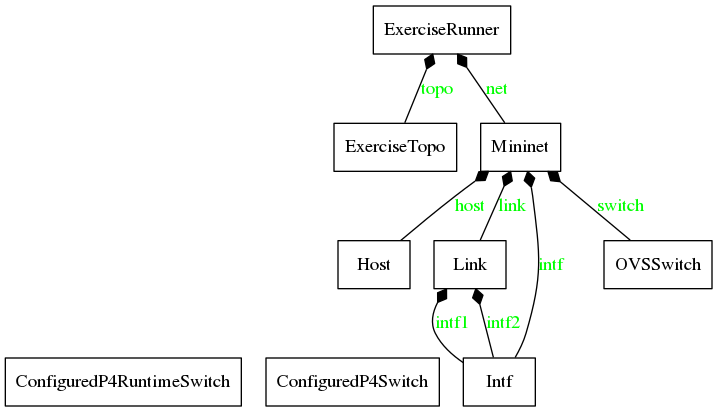
\includegraphics[width=13cm]{archivos/img/dev/p4-wifi/analysis/run_exercise_pertenencia.png}
    \caption{UML del punto de entrada de la interfaz BMv2 - Mininet}
    \label{fig:analysis_p4_wifi_1}
\end{figure}

%uml_2
% figura escenario
\begin{figure}[h!]
    \centering
    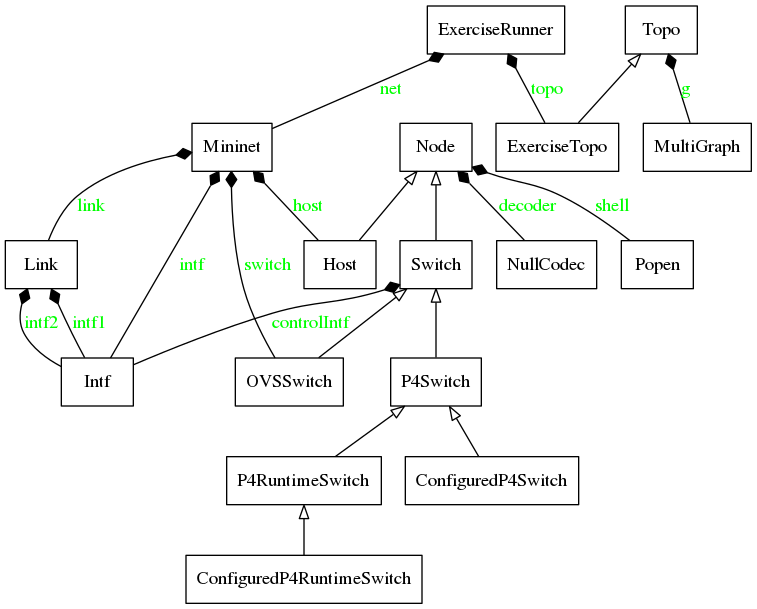
\includegraphics[width=13.5cm]{archivos/img/dev/p4-wifi/analysis/run_exercise_class_names_only.png}
    \caption{UML interfaz BMv2 - Mininet}
    \label{fig:analysis_p4_wifi_2}
\end{figure}



\subsubsection{Análisis del funcionamiento interno de Mininet-WiFi}

Una vez que se revisó el funcionamiento interno de la API de Mininet-P4, se da paso a analizar Mininet-WiFi en profuncidad. Como se comentaba en el capítulo \ref{estadoArte}, Mininet-WiFi es una herramienta de emulación de redes wireless que ha nacido de Mininet, es decir es un fork de este. Al ser un fork comparte gran parte de la jerarquía de clases así como su capacidad para simular ciertos elementos de la red. Aun así, si bien se ha mencionado en numerosas ocasiones que Mininet-WiFi esta desarrollado a partir de Mininet, la capacidad de emulación de interfaces \textit{Wireless} la toma de subsistema wireless de Linux.\\
\par

La arquitectura de virtualización empleada en Mininet-WiFi funciona de forma similar a la Mininet; se hace uso de la herramienta \texttt{mnexec}\footnote{\url{https://github.com/intrig-unicamp/mininet-wifi/blob/master/mnexec.c}} para lanzar distintos procesos de bash en nuevas \textit{Network Namespaces}, uno por cada nodo independiente de la red. De estos procesos colgarán todos los procesos relativos a los distintos nodos de la red. Cuando la emulación haya terminado, se matarán dichos procesos de bash, consiguiendo que no haya ninguna condición de referenciación de las \textit{Network Namespaces}, y estas sean eliminadas por el Kernel.\\
\par

De esta manera, los nodos de la red ya estarían aislados entre sí, por loque lo único que quedaría por virtualizar son las capacidades \textit{wireless} de los nodos que las requieran. Para ellos se hará uso del subsistema \textit{wireless}  del Kernel de Linux, más concretamente el módulo \texttt{mac80211\_hwsim} el cual creará las interfaces \textit{wireless}  en nuestro equipo. Este módulo se comunicará con framework \texttt{mac80211} el cual proveerá de las capacidades de gestión de acceso al medio de la interfaz \textit{wireless} . Además, en el espacio de Kernel aun hay un bloque más, llamado cfg80211, el cual servirá de API para la configuración de las cabeceras 802.11. Esta configuración puede ser realizada por la interfaz netlink de espacio de usuario llamada nl80211. Para la configuración de los puntos de acceso, se hará uso del programa \texttt{HostApd} el cual indicándole la configuración del punto de acceso y la interfaz sobre la cual debe correr, emulará el funcionamiento de un punto de acceso estándar. En la  figura \ref{fig:analysis_p4_wifi_3} se puede ver de manera resumida la arquitectura básica de Mininet-WiFi.\\
\par

% foto arch Mininet-wifis
% figura escenario
\begin{figure}[ht]
    \centering
    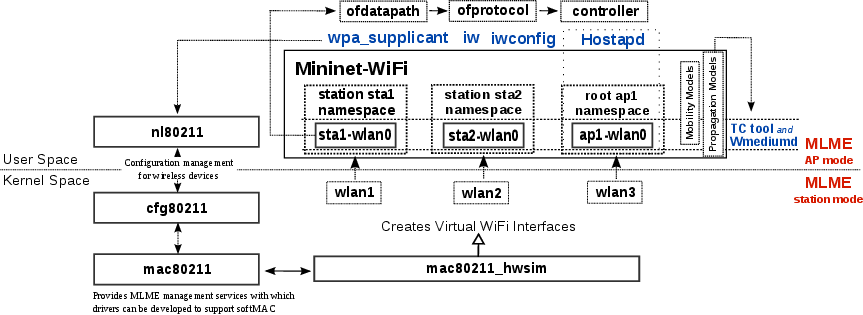
\includegraphics[width=15cm]{archivos/img/dev/p4-wifi/analysis/mininet_wifi_components.png}
    \caption{Arquitectura Mininet-WiFi \cite{7367387}}
    \label{fig:analysis_p4_wifi_3}
\end{figure}


En cuanto a la jerarquía de clases,únicamente cabe mencionar que es bastante similar a la de Mininet. Por destacar dos clases claves en la jerarquía de Mininet-WiFi, serían Node\_Wifi, de la cual heredan todos los nodos con capacidades wireless que posee Mininet-WiFi y por último, la clase IntfWireless, de la cual heredan todos los tipos de enlaces disponibles de Mininet-WiFi (Bajo el estándar \texttt{ieee80211}). A continuación,  en la figuras \ref{fig:analysis_p4_wifi_4} y \ref{fig:analysis_p4_wifi_5}, se indican los UML referentes a dichas clases.\\
\par

% uml_3 wifis
% figura escenario
\begin{figure}[ht]
    \centering
    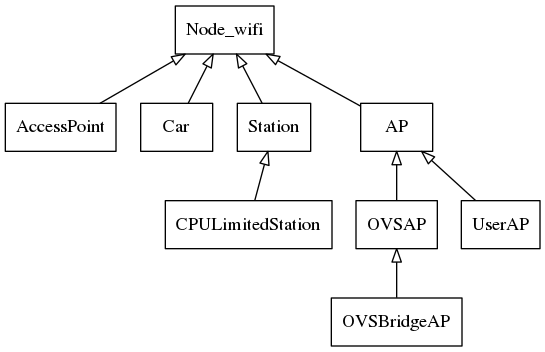
\includegraphics[width=8cm]{archivos/img/dev/p4-wifi/analysis/uml_node.png}
    \caption{UML sobre las relaciones de las clases de tipo Nodo.}
    \label{fig:analysis_p4_wifi_4}
\end{figure}



Como se puede apreciar en los esquemas UML, se ha conseguido aislar la funcionalidad común en las clases padres, con la finalidad de optimizar la cantidad de código de las clases hijas. De esta forma, añadir nuevos tipos de enlaces y nodos en Mininet-WiFi resulta bastante asequible.\\
\par

% uml_4 wifis
% figura escenario
\begin{figure}[ht]
    \centering
    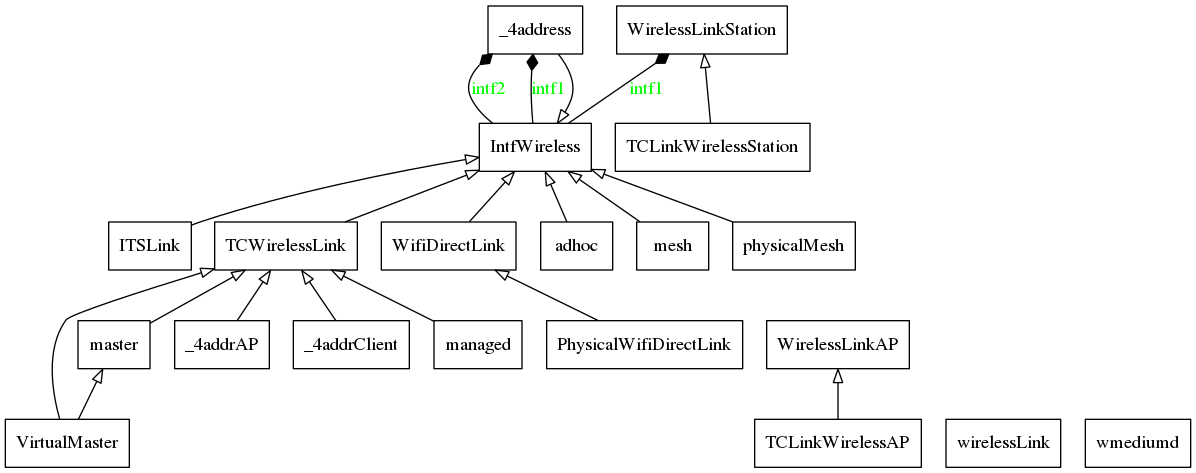
\includegraphics[width=15cm]{archivos/img/dev/p4-wifi/analysis/uml_link.png}
    \caption{UML sobre las relaciones de las clases de tipo Interfaz.}
    \label{fig:analysis_p4_wifi_5}
\end{figure}



\vspace{1cm}
\textbf{Linux Wireless Subsystem}\\
\par

El subsistema \textit{wireless} de Linux consiste en un set de varios módulos que se encuentran en el Kernel de Linux. Estos manejan la configuración del hardware bajo el estándar \texttt{ieee80211}, además de la gestión de la transmisión y la escucha de los paquetes de datos. Yendo de desde abajo hacia arriba en la arquitectura del subsistema, el primer bloque que se encuentra es el módulo mac80211\_hwsim. Este módulo como ya se comentaba es el responsable de crear las interfaces \textit{wireless} virtuales en Mininet-WiFi.\\
\par

% arch LWS
% figura escenario
\begin{figure}[ht]
    \centering
    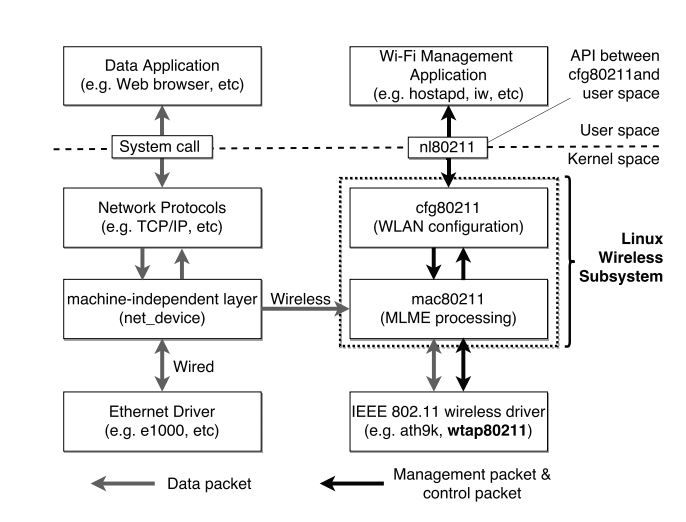
\includegraphics[width=14cm]{archivos/img/dev/p4-wifi/analysis/linux_wireless_subsystem.JPG}
    \caption{Arquitectura del subsistema Wireless de Linux \cite{8330098}}
    \label{fig:analysis_p4_wifi_6}
\end{figure}

El objetivo principal de este módulo mac80211\_hwsim es facilitar a los desarrolladores de drivers de tarjetas \textit{wireless} la prueba de su código e interacción con el siguiente bloque llamado mac80211. Las interfaces virtualizadas no tienen ciertas limitaciones, es decir, a diferencia del hardware real, resulta más sencillo la creación de distintas pruebas con distintas configuraciones sin estar cohibidos por falta de recursos materiales. Este módulo generalmente recibe un único parámetro, que es el número de ``radios", interfaces virtuales, a virtualizar. Dado que las posibilidades que ofrece este módulo eran un poco reducidas, muchos \textit{wrappers} (``envoltorios al software original") han sido creados para ofrecer más funcionalidad a parte de la dada por el propio módulo. La mayoría de herramientas creadas hacen uso de la librería Netlink para comunicarse directamente con el subsistema en el Kernel y así conseguir configuraciones extra, como pueden ser añadir un \gls{rssi} o darle nombre a la interfaz. Un ejemplo de dichas herramientas sería la herramienta \texttt{mac80211\_hwsim\_mgmt}, la cual es usada por Mininet-WiFi para gestionar la creación de las interfaces \textit{wireless} en cada nodo que las requiera.\\
\par

Es importante mencionar el cambio de paradigma que existe en el subsistema \textit{wireless} de Linux con el concepto de interfaz. Generalmente se está acostumbrado a pensar en el concepto de interfaz como un elemento que gestiona el acceso al medio, capa dos, y el propio hardware, capa física, un ejemplo de ello sería una interfaz de Ethernet. Bien, pues en el subsistema wireless se desglosa la interfaz en dos capas \cite{8330098}. Una de ellas es la capa física (\textit{PHY}) donde se puede gestionar por ejemplo en que canal está escuchando la tarjeta wireless emulada. La otra capa es el acceso al medio, representado por las interfaces virtuales que ``cuelgan" de una tarjeta wireless.\\
\par
 La idea detrás de este paradigma, es que puede tener \textit{N} interfaces virtuales asociadas a la misma tarjeta WiFi emulada, lo que resultó sorprendente es que las interfaces virtuales funcionan principalmente con Ethernet (dejando de lado las que están en modo monitor).

\vspace{0.5cm}
\textbf{Limitaciones encontradas}\\
\par
\label{limitacionesEncontradas}

Como ya se ha comentado, la mayoría de interfaces virtuales asociadas a una tarjeta wireless emulada son del tipo de Ethernet, por lo que todos los paquetes que llegan vienen con cabeceras Ethernet. Esto supone una limitación ya que en los casos de uso se quería gestionar las cabeceras WiFi, pero si todas las interfaces virtuales son generalmente del de tipo Ethernet, no será posible.

% foto downstream
% figura escenario
\begin{figure}[ht]
    \centering
    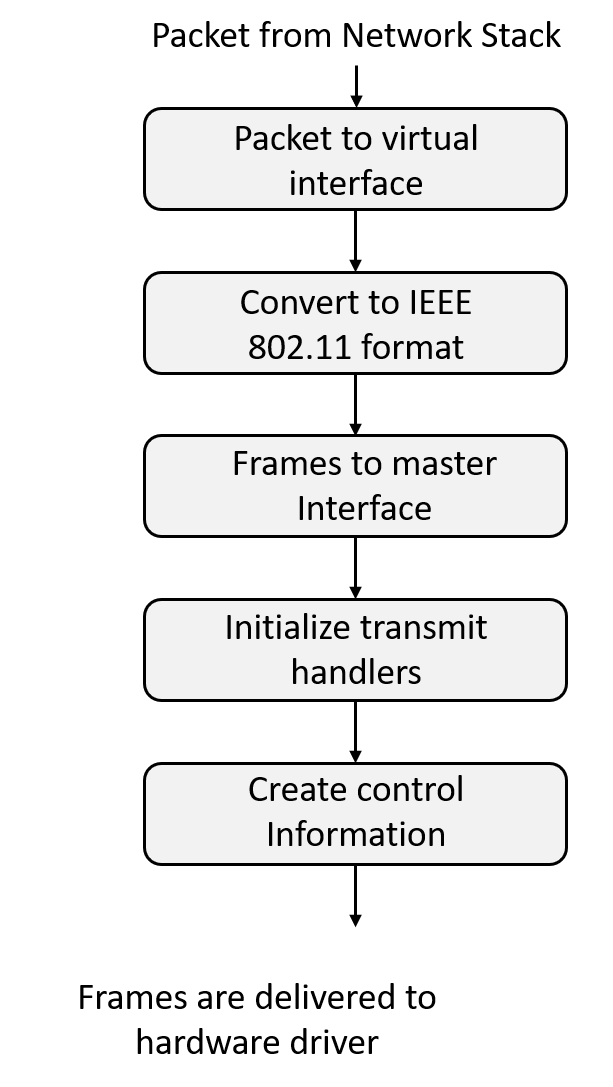
\includegraphics[width=4cm]{archivos/img/dev/p4-wifi/analysis/linux_wireless_subsystem_tx.png}
    \caption{Flujo para la transmisión con el módulo mac80211\_hwsim \cite{5415877}}
    \label{fig:analysis_p4_wifi_7}
\end{figure}

Pero, ¿Qué sentido tiene tener convertir las cabeceras WiFi a cabeceras Ethernet? De momento la única razón que se ha encontrado de esta decisión de diseño, es hacer un diseño más sencillo de todos los drivers que operan bajo el módulo mac80211\_hwsim, que convierten a Ethernet y se lo entregan al stack de red para que lo gestione como un paquete más de una red cableada. De esta forma, las aplicaciones que operen a nivel de interfaz serán más extrapolables. 

% foto upstream
% figura escenario
\begin{figure}[ht]
    \centering
    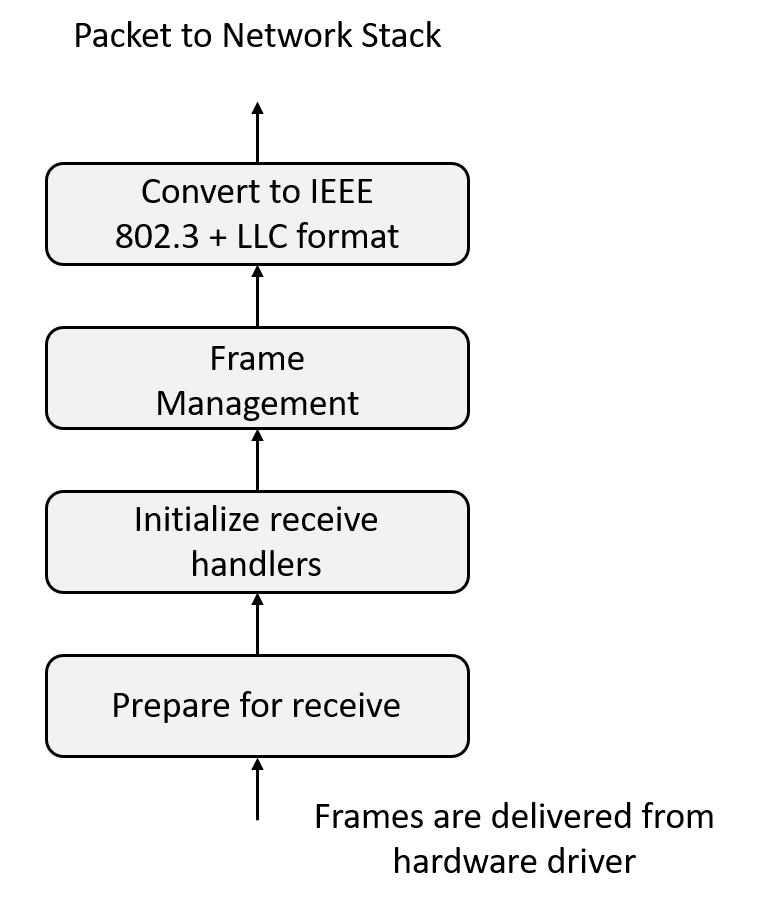
\includegraphics[width=5cm]{archivos/img/dev/p4-wifi/analysis/linux_wireless_subsystem_rx.png}
    \caption{Flujo para la recepción con el módulo mac80211\_hwsim \cite{5415877}}
    \label{fig:analysis_p4_wifi_8}
\end{figure}

Pero, hay que mencionar que esto supone un gasto de recursos considerable, ya que el paquete es encolado hasta tres veces (driver, ethernet queue, qdisc queue) y se tiene que invertir tiempo y recursos en el proceso de traducción de las cabeceras.  \href{https://elixir.bootlin.com/linux/latest/C/ident/__ieee80211_data_to_8023}{\textbf{Aquí}}\footnote{\url{https://elixir.bootlin.com/linux/latest/C/ident/__ieee80211_data_to_8023}} se puede ver la función en el kernel donde se lleva a cabo ese proceso.\\
\par

Esto sucede generalmente y no siempre ya que en el único modo que una interfaz puede llegar a escuchar los paquetes WiFi es en el modo monitor. Pero el modo monitor está pensado únicamente para escuchar paquetes, no para transmitir. Este modo puede ser llevado al limite haciendo una inyección de paquetes (packet injection) por la interfaz.\\
\par

De esta forma se conseguiría el objetivo de manejar las cabeceras WiFi, pero dadas las competencias del \gls{tfg}, este desarrollo se escapa completamente. Ni si quiera Mininet-WiFi, siendo la herramienta de facto para emular redes \textit{wireless}, contempla el manejo de cabeceras WiFi. Por ello, este objetivo se plantea como un desarrollo a posteriori y se mencionará en el trabajo futuro (Ver sección \ref{trabajoFuturo}). \\
\par
El desarrollo pues sobre Mininet-WiFi, consistirá en la integración del \gls{bmv2} en Mininet-WiFi, y probar los casos de uso desarrollados para P4, bajo Mininet-WiFi. Las cabeceras que llegarán a la pipeline serán las de Ethernet, pero como ya se ha explicado, es el propio Kernel quien se encarga de hacer un \textit{casting} de las cabeceras WiFi hacia cabeceras Ethernet.\\
\par

\subsubsection{Desarrollo de la interfaz BMV2 - Mininet-WiFi}

Ahora que ya se tiene una idea sobre el funcionamiento interno de ambas herramientas, vamos a proceder a su integración. A la par que se estaba trabajando en el desarrollo de la integración del \gls{bmv2} en Mininet-WiFi, el investigador Ramon Fontes (desarrollador de la herramienta) abrió un Issue (es decir, una publicación de debate y ampliación de funcionalidad de GitHub) donde se exponía la intención de crear dicha integración. En este issue se pudo debatir con Ramon Fontes cómo debía hacerse dicho desarrollo.\\
\par

En concreto, se decidió hacer un jerarquía de clases genérica para el \gls{bmv2} para que de estas se puedan crear clases personalizadas con añadidos nuevos. Por así decirlo, estas clases serán la base para clases que controlen el \gls{bmv2} de una forma más particular.\\
\par
Una clase \texttt{P4AP}, la cual contiene todos los atributos y métodos comunes al \gls{bmv2} como son el path de ejecución del \gls{bmv2}, el json compilado del programa P4, el thrift-port, configuración de log y identificador básico del \gls{bmv2}. De esta clase se quiere que herede una clase llamada \texttt{P4RuntimeAP}, la cual proporcionará todos los elementos necesarios para dar soporte a la configuración vía P4Runtime vía gRPC-port del \gls{bmv2}.\\
\par

% Foto uml propio
% figura escenario
\begin{figure}[ht]
    \centering
    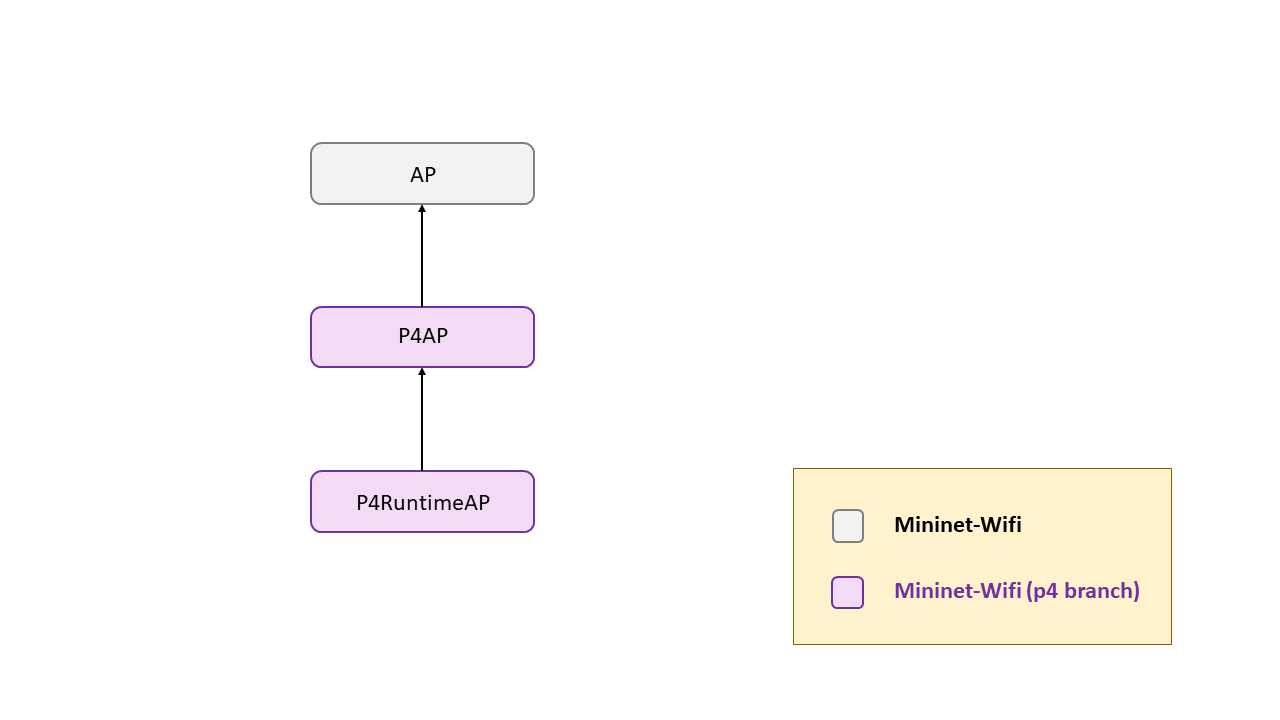
\includegraphics[width=15.5cm]{archivos/img/dev/p4-wifi/analysis/p4_Mininet_Wifi_UML.png}
    \caption{UML de la integración BMv2 - Mininet-WiFi}
    \label{fig:analysis_p4_wifi_9}
\end{figure}

Además debatiendo con Ramon Fontes sobre la implementación de estas clases,  indicó que sería de gran utilidad que dichas clases tuvieran soporte de ejecución en Network Namespaces, por lo que de forma paralela se tuvo que crear una clase llamada \texttt{Netns\_mgmt}\footnote{\url{https://github.com/davidcawork/TFG/tree/master/src/netns_mgmt}}. Esta clase ayudará a gestionar la ejecución de código Python en \textit{runtime} en una Network namespace indicada haciendo uso de la llamada al sistema \textbf{setns} la cual asocia el procesos sobre la cual se realiza esta llamada, a una \textit{Namespace} indicada.\\
\par

Con la ayuda de esta clase, \texttt{Netns\_mgmt}, se pudo conseguir configurar cada \gls{bmv2} en su propia \textit{Network Namespace}, por lo que la integración se dio por terminada. Adicionalmente se añadieron dos ejemplos a Mininet-WiFi con la finalidad de ayudar a las personas que vayan hacer uso de clase. Dichos ejemplos pueden ser encontrados \href{https://github.com/davidcawork/mininet-wifi/tree/p4/examples/p4}{\textbf{aquí}}.\footnote{\url{https://github.com/davidcawork/mininet-wifi/tree/p4/examples/p4}}\\
\par
Todo este desarrollo se llevo a cabo en un fork de Mininet-WiFi, y dentro de este en una rama en particular, en la cual se llevan a cabo todos los desarrollos de P4. Una vez finalizada la integración, se ofreció el desarrollo al repositorio oficial de Mininet-WiFi vía pull-request. Actualmente se ha dejado a la espera de hacer un \textit{upgrade} a las dependencias donde fue llevada a cabo la integración, ya que Mininet-WiFi está trabajando con las últimas versiones. En cambio, para el desarrollo de los casos de uso P4-wireless, se hará uso de las últimas versiones  estables de las dependencias del entorno P4.

\vspace{1cm}
\textbf{Puesta en marcha del Mininet-WiFi modificado}\\
\par
\label{mn_wifi_own_deps}

Para poder probar el desarrollo llevado a cabo con Mininet-WiFi se deberán seguir los pasos indicados en el bloque \ref{code:wifi_bmv2_integration_deps} previamente. Se deberá bajar el repositorio del fork de Mininet-WiFi. Se hará un checkout para moverse desde la rama master del repositorio a la rama de desarrollo de elementos P4.

\begin{lstlisting}[language= bash, style=Consola, caption={Instalación de Mininet-WiFi modificado},label=code:wifi_bmv2_integration_deps]
    # Se descarga el repositorio
    git clone https://github.com/davidcawork/mininet-wifi
    
    # Se adquieren las etiquetas y se cambia de rama
    cd mininet-wifi && git fetch
    git checkout p4
    
    # Se "recompilará" Mininet-Wifi
    sudo make install
\end{lstlisting}
\vspace{0.5cm}

Como la rama de desarrollo añade módulos nuevos a Mininet-WiFi se deberá ``recompilar" de nuevo haciendo un make install desde el directorio \texttt{/mininet-wifi}. Para que los módulos añadidos funcionen correctamente se deberán tener las dependencias del entorno P4, en la tabla \ref{tab:mn-wifi_bmv2_integration_deps} se pueden comprobar que versiones son requeridas.\\
\par

\begin{table}[ht]
\centering

\begin{tabular}{|c|c|}
\hline
\rowcolor[HTML]{EFEFEF} 
{\color[HTML]{24292E} \textbf{Dependencia}} & {\color[HTML]{24292E} \textbf{Versión requerida}} \\ \hline
\href{https://github.com/p4lang/behavioral-model}{\textbf{BMV2}}                                        & \texttt{b447ac4c0cfd83e5e72a3cc6120251c1e91128ab}          \\ \hline
\href{https://github.com/p4lang/PI}{\textbf{PI}}                                          & \texttt{41358da0ff32c94fa13179b9cee0ab597c9ccbcc}          \\ \hline
\href{https://github.com/p4lang/p4c}{\textbf{P4C}}                                         & \texttt{69e132d0d663e3408d740aaf8ed534ecefc88810}         \\ \hline
\href{https://github.com/protocolbuffers/protobuf}{\textbf{PROTOBUF}}                                    & \texttt{v3.2.0}                                        \\ \hline
\href{https://github.com/grpc}{\textbf{GRPC}}                                        & \texttt{v1.3.2}                                           \\ \hline
\end{tabular}%
\caption{Resumen de las versiones requeridas de la interfaz BMv2 - Mininet-WiFi}
\label{tab:mn-wifi_bmv2_integration_deps}
\end{table}


\subsection{Case01 - Drop}
\label{p4_wifi_case01}

En este caso de uso se probará que es posible descartar todos los paquetes recibidos con un programa P4 en una interfaz virtual \textit{Wireless}. Como tal el programa P4 no es suficiente para probar esta funcionalidad ya que requiere de una plataforma que sea capaz de soportar el lenguaje P4. Se hará uso de software switch llamado behavioral-model, \gls{bmv2} en adelante, para testear los programas P4, y de la integración desarrollada anteriormente con Mininet-WiFi como escenario para recrear las topologías de Red.\\
\par

Como este caso de uso ya se ha explicado anteriormente en el case01 de P4 cableado (Ver subsección \ref{p4_ether_case01}), y no hay ninguna diferencia inducida en el cambio de entorno según se explico en las sección anterior,  únicamente se harán indicaciones sobre como poder compilarlo y ejecutarlo. Importante, si usted está replicando este caso de uso, sin antes haber adecuado las dependencias necesarias de Mininet-WiFi con soporte del \gls{bmv2}, vuelva a este punto \ref{mn_wifi_own_deps} y siga los pasos indicados.

% figura escenario
\begin{figure}[ht]
    \centering
    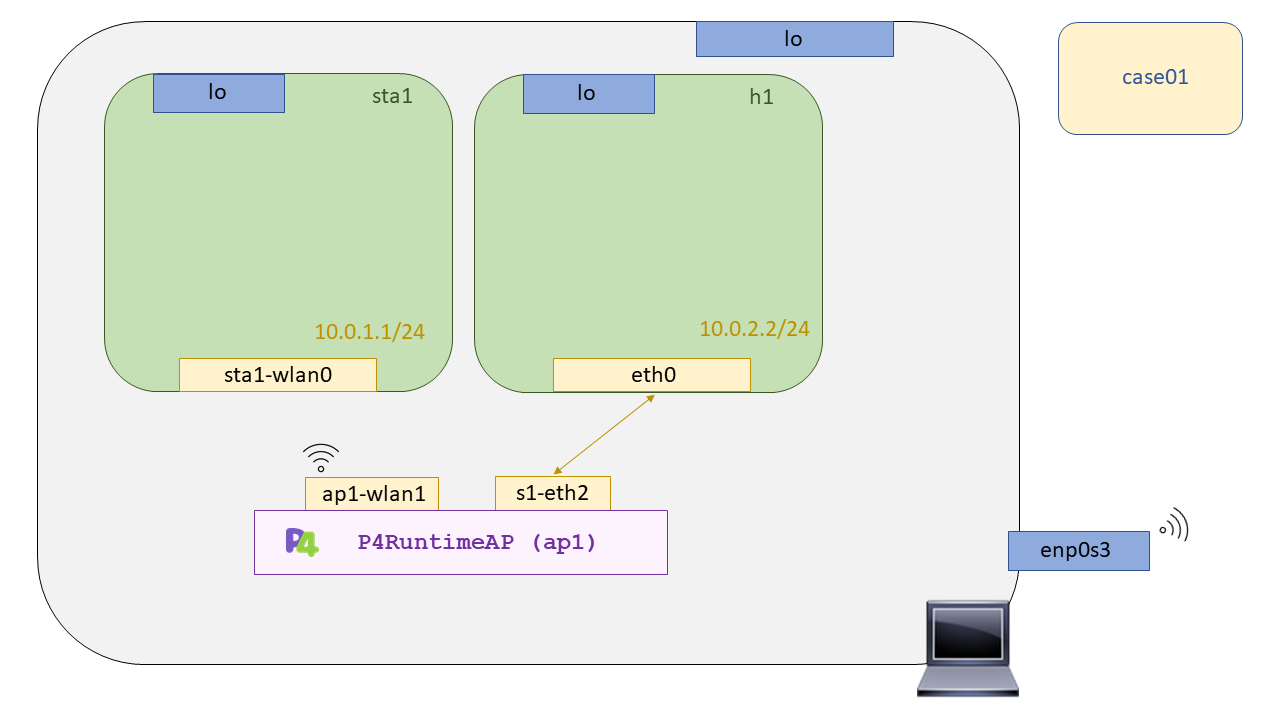
\includegraphics[width=16cm]{archivos/img/dev/p4-wifi/case01/scenario.png}
    \caption{Escenario del Case01 - P4 Wireless}
    \label{fig:case01_p4_wifi_scenario}
\end{figure}

\vspace{0.2cm}
\textbf{Compilación}\\
\par

Para la compilación de este caso de uso, se ha dejado preparado un Makefile, por tanto no es necesario que el usuario aprenda a utilizar el compilador p4c. Si se quiere saber más sobre como funciona el proceso de compilación, qué etapas hay, como se le "inyecta" el \texttt{json} generado al \gls{bmv2}, o qué distintos \textit{targets} hay en función de la arquitectura, le recomendamos que vuelva al case01 (\ref{p4_ether_case01}). Para llevar a cabo la compilación solo se tendrá que seguir los pasos indicados en el bloque \ref{code:case01_p4_wifi_load}.

\begin{lstlisting}[language= bash, style=Consola, caption={Compilación programa P4  - Case01},label=code:case01_p4_wifi_load]
    # Entramos al directorio 
    cd TFG/src/use_cases/p4-wireless/case01

    # Hacemos uso del Makefile
    sudo make
\end{lstlisting}
\vspace{0.5cm}


Una vez ejecutado el make, se habrá generado una estructura de directorios que se utilizarán en el lanzamiento del caso de uso. Bajo el directorio \texttt{build} se podrá encontrar el \texttt{json} generado por el compilador, será este \texttt{json} quien tenga toda la información requerida para conformar el \gls{bmv2}.\\
\par

\vspace{0.2cm}
\textbf{Puesta en marcha del escenario}\\
\par

Al igual que en la compilación, se ha dejado preparado un script en Python para automatizar la puesta en marcha del escenario. Este script describe la topología que se utilizará en este caso de uso. Recordemos que es necesario volver hacer un \texttt{make install} para instalar los módulos adicionales generados para la integración del \gls{bmv2} y Mininet-WiFi, además de tener instaladas las versiones indicadas en el análisis de la integración. Estas dependencias se pueden encontrar en el apartado \ref{mn_wifi_own_deps} \\
\par

Una vez comprobado que posee todas la dependencias, simplemente se tendrá que ejecutar el script con el interprete de Python. Este script levantará la topología descrita en la figura \ref{fig:case01_p4_wifi_scenario}, compuesto por dos hosts y por una instancia del nodo \texttt{P4RuntimeAP}. El nodo \texttt{ap1}, del tipo \texttt{P4RuntimeAP}, tendrá dos interfaces, una wireless y un par de \gls{veth}.



\begin{lstlisting}[language= bash, style=Consola, caption={Puesta en marcha del escenario  - Case01},label=code:case01_p4_wifi_run]
    sudo python scenario.py
\end{lstlisting}
\vspace{0.2cm}


\vspace{0.5cm}
\textbf{Comprobación del funcionamiento}\\
\par

Tras las ejecución del script \texttt{scenario.py}, se tendría el escenario \ref{fig:case01_p4_wifi_scenario} levantado, y la CLI de Mininet-WiFi abierta. Para la comprobación de funcionamiento de este caso de uso, se van a seguir los mismos pasos que en el case01 (\ref{p4_ether_case01}) - P4 en un entorno alámbrico. Por tanto no se entrará en hacer explicaciones que se creen redundantes, se indicarán los pasos seguidos para llevar a cabo la comprobación de funcionamiento y los resultados de dichas pruebas. 

\begin{lstlisting}[language= bash, style=Consola, caption={Pasos a seguir para comprobar el funcionamiento - Case01},label=code:case01_p4_wifi_func1]
    mininet-wifi>  xterm sta1 h1
    
    # Se hará ping desde la estación Wifi al Host
    [sta1] ping 10.0.2.2
    
    
    # Se pondrá a escuchar en el Host
    [h1] tcpdump -l

\end{lstlisting}
\vspace{0.5cm}


% Figura
% figura escenario
\begin{figure}[ht]
    \centering
    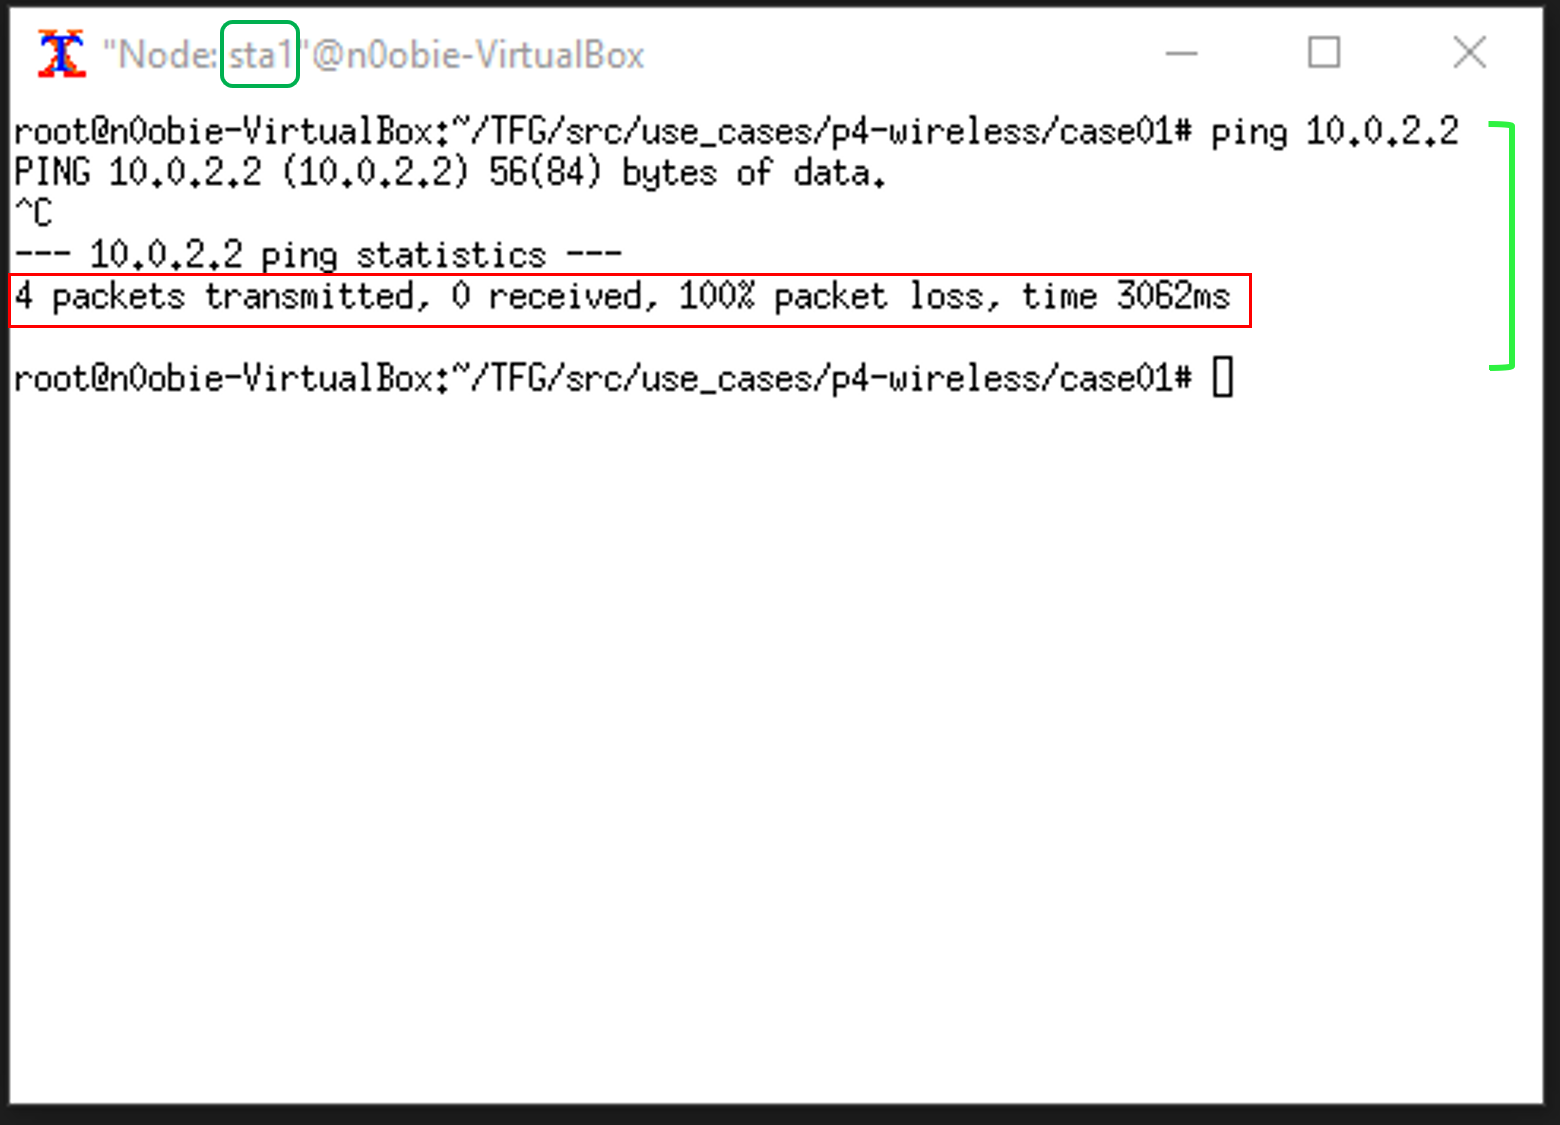
\includegraphics[width=14cm]{archivos/img/dev/p4-wifi/case01/demo_case01_1_edited.png}
    \caption{Comprobación de funcionamiento (Ping) del Case01 - P4 Wireless}
    \label{fig:case01_p4_wifi_func1}
\end{figure}
\vspace{0.5cm}

Como se puede ver en la figura \ref{fig:case01_p4_wifi_func1}, no hay conectividad entre ambos nodos dado que el ping \fcolorbox{black}{green}{\rule{0pt}{2.5pt}\rule{2.5pt}{0pt}}\hspace{1mm} no está llegando. Por lo que, el programa P4 está funcionando según lo esperado, tirando los paquetes que llegan a su \textit{pipeline} de procesamiento. Para asegurarse de que realmente se está ejecutando el \textit{action} para tirar paquetes podemos consultar los logs del \gls{bmv2}, los cuales generan un fichero de log por cada instancia \textit{target} del \texttt{P4RuntimeAP} que se haya levantado.\\
\par

\newpage

\begin{figure}[ht]
    \centering
    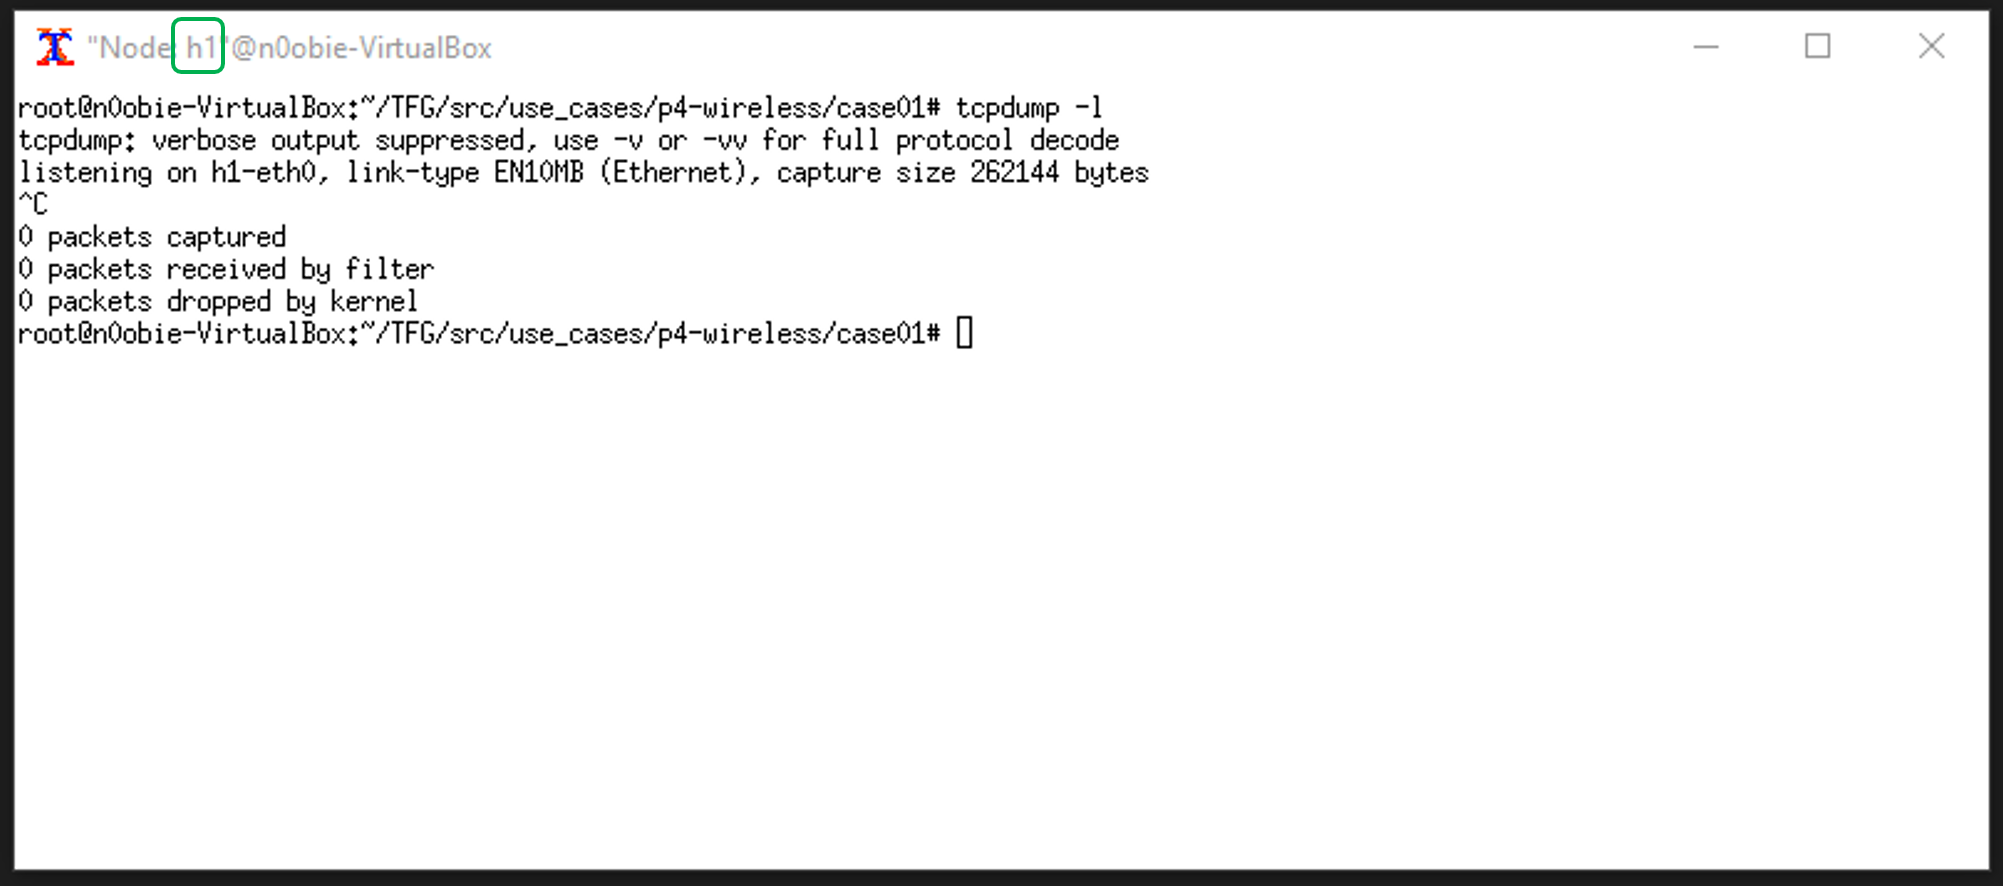
\includegraphics[width=14cm]{archivos/img/dev/p4-wifi/case01/demo_case01_2_edited.png}
    \caption{Comprobación de funcionamiento (Sniffer) del Case01 - P4 Wireless}
    \label{fig:case01_p4_wifi_func2}
\end{figure}
\subsection{Case02 - Pass}
\label{p4_wifi_case02}


Como se puede apreciar, en este directorio no hay ningún programa P4, al igual que en caso de uso P4, case02 (\ref{P4_ether_case02}),  en entornos cableados. Esto se debe a que no hay equivalente en P4 del código de retorno \texttt{XDP\_PASS}, por ello, no se puede hacer nada en este caso de uso. El código de de retorno en \gls{xdp} es una forma para llevar a cabo una acción con el paquete que llega a la interfaz, en la cual hay anclado un programa \gls{xdp}. En este caso el código de retorno  \texttt{XDP\_PASS} implica que el paquete se pasa al siguiente punto del procesamiento del \textit{stack} de red en el Kernel de Linux. Es decir, si el programa está anclado a la \gls{nic}, se dejará pasar el paquete al \gls{tc}, de ahí al propio \textit{stack} de red para parsear sus cabeceras, y más adelante, dárselo de comer a la interfaz de sockets.\\
\par

En P4, el entorno donde se llevaran a cabo los casos de uso será Mininet-WiFi con \gls{ap}s (\gls{bmv2}) y host. Los \gls{ap}s (\gls{bmv2}) son un software switch en los que podemos inyectar código P4, con el cual podemos definir el \textit{datapath} del mismo.\\
\par

Ahora bien, aquí viene la gran diferencia entre ambas tecnologías, con \gls{xdp} siempre es posible pasarle el paquete al Kernel para que se encargue el del procesamiento, pero en P4, debemos definir nosotros de forma exclusiva todo el \textit{datapath}, por lo que no hay a quien delegar el paquete, se debe encargar el propia programa P4. Entonces, como tal, no habría equivalente del  \texttt{XDP\_PASS} en P4, como es obvio ni en escenarios cableados ni inalámbricos, es una característica de la propia tecnología.\\
\par
\subsection{Case03 - Echo server}
\label{p4_wifi_case03}

 En este caso de uso desarrollaremos un servidor de echo que responda todos los pings que le lleguen al \gls{bmv2}. Como tal el programa P4 no es suficiente para probar esta funcionalidad ya que requiere de una plataforma que sea capaz de soportar el lenguaje P4. Se hará uso de software switch \gls{bmv2}, para testear los programas P4, y de la integración desarrollada anteriormente con Mininet-WiFi como escenario para recrear las topologías de Red. Como el \gls{bmv2} será configurado vía P4Runtime se hará uso de la clase de \texttt{P4RuntimeAP}.\\
\par

Dado que este caso de uso ya se ha explicado anteriormente en el case03 de P4 cableado (Ver subsección \ref{P4_ether_case03}), y no hay ninguna diferencia inducida en el cambio de entorno según se explico en las sección anterior,  únicamente se harán indicaciones sobre como poder compilarlo y ejecutarlo. Importante, si usted está replicando este caso de uso, sin antes haber adecuado las dependencias necesarias de Mininet-WiFi con soporte del \gls{bmv2}, vuelva a este punto \ref{mn_wifi_own_deps} y siga los pasos indicados.\\
\par

% figura escenario
\begin{figure}[ht]
    \centering
    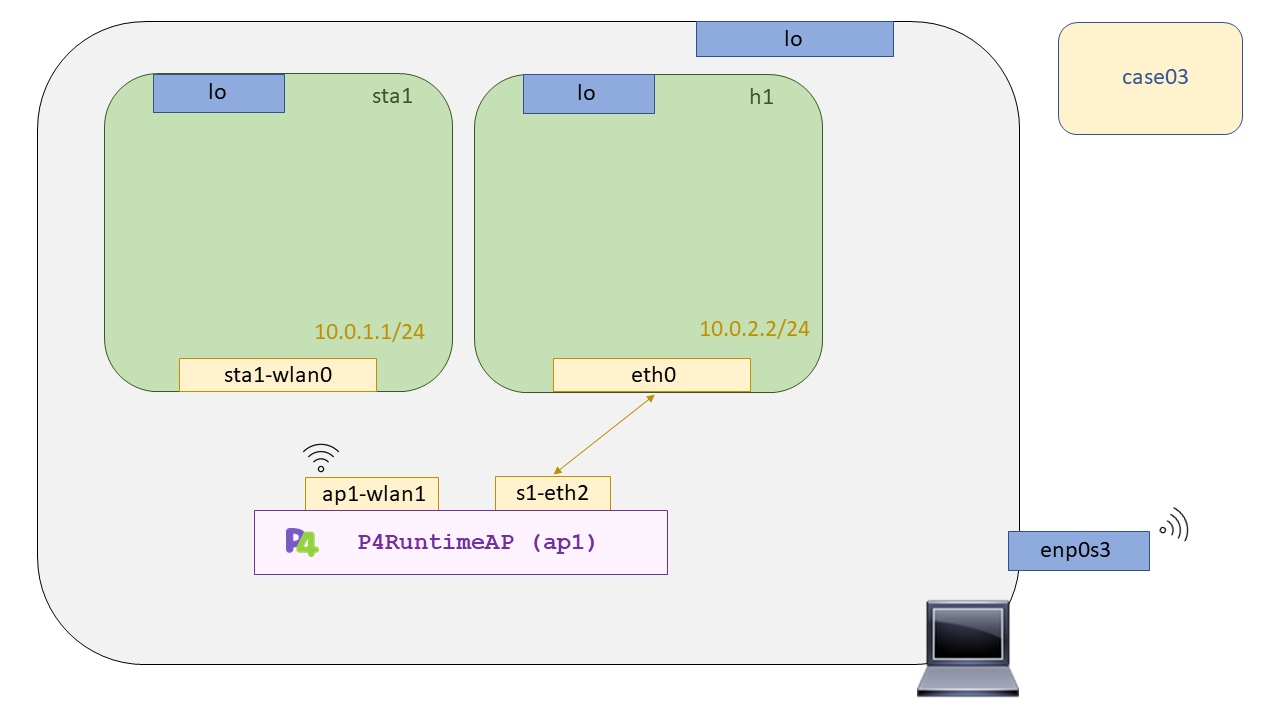
\includegraphics[width=16cm]{archivos/img/dev/p4-wifi/case03/scenario.png}
    \caption{Escenario del Case03 - P4 Wireless}
    \label{fig:case03_p4_wifi_scenario}
\end{figure}

\vspace{0.2cm}
\textbf{Compilación}\\
\par

Para la compilación de este caso de uso, al igual que en los casos de uso anteriores se ha dejado preparado un Makefile, por tanto no es necesario que el usuario haga un uso directo del compilador p4c. Si se quiere saber más sobre como funciona el proceso de compilación, qué etapas hay, como se le ``inyecta" el \texttt{json} generado al \gls{bmv2}, o qué distintos \textit{targets} hay en función de la arquitectura, le recomendamos que vuelva al case01 (\ref{p4_ether_case01}). Para llevar a cabo la compilación solo se tendrá que seguir los pasos indicados en el bloque \ref{code:case03_p4_wifi_load}.

\newpage

\begin{lstlisting}[language= bash, style=Consola, caption={Compilación programa P4  - Case03},label=code:case03_p4_wifi_load]
    # Entramos al directorio 
    cd TFG/src/use_cases/p4-wireless/case03

    # Hacemos uso del Makefile
    sudo make
\end{lstlisting}
\vspace{0.3cm}


Una vez ejecutado el make, se habrá generado una estructura de directorios que se utilizarán en el lanzamiento del caso de uso. Bajo el directorio \texttt{build} se podrá encontrar el \texttt{json} generado por el compilador, será este \texttt{json} quien tenga toda la información requerida para conformar el \gls{bmv2}. Los directorios \texttt{log} y \texttt{pcap}, se utilizarán respectivamente para almacenar los logs del \gls{bmv2} y para guardar las capturas de paquetes de las interfaces asociadas a la instancia \gls{bmv2}.\\
\par



\vspace{0.2cm}
\textbf{Puesta en marcha del escenario}\\
\par

Al igual que en la compilación, se ha dejado preparado un script en Python para automatizar la puesta en marcha del escenario. Este script describe la topología que se utilizará en este caso de uso. Recordar que es necesario volver hacer un \texttt{make install} para instalar los módulos adicionales generados para la integración del \gls{bmv2} y Mininet-WiFi, además de tener instaladas las versiones indicadas en el análisis de la integración. Estas dependencias se pueden encontrar en el apartado \ref{mn_wifi_own_deps}. Una vez comprobado que posee todas la dependencias, simplemente se tendrá que ejecutar el script con el interprete de Python. Este script levantará la topología descrita en la figura \ref{fig:case03_p4_wifi_scenario}, compuesto por dos estaciones WiFi y por una instancia del nodo \texttt{P4RuntimeAP}. El nodo \texttt{ap1}, del tipo \texttt{P4RuntimeAP}, tendrá dos interfaces, una wireless y un par de \gls{veth}.


\begin{lstlisting}[language= bash, style=Consola, caption={Puesta en marcha del escenario  - Case03},label=code:case03_p4_wifi_run]
    sudo python scenario.py
\end{lstlisting}

\vspace{0.4cm}
\textbf{Comprobación del funcionamiento}\\


Tras las ejecución del script \texttt{scenario.py}, se tendría el escenario \ref{fig:case03_p4_wifi_scenario} levantado, y la CLI de Mininet-WiFi abierta. Para la comprobación de funcionamiento de este caso de uso, se van a seguir los mismos pasos que en el case03 (\ref{P4_ether_case03}) - P4 en un entorno alámbrico, adaptados en Mininet-WiFi. Por tanto solo se indicarán los pasos seguidos para llevar a cabo la comprobación de funcionamiento y los resultados de dichas pruebas. 

% figura escenario
\begin{figure}[ht]
    \centering
    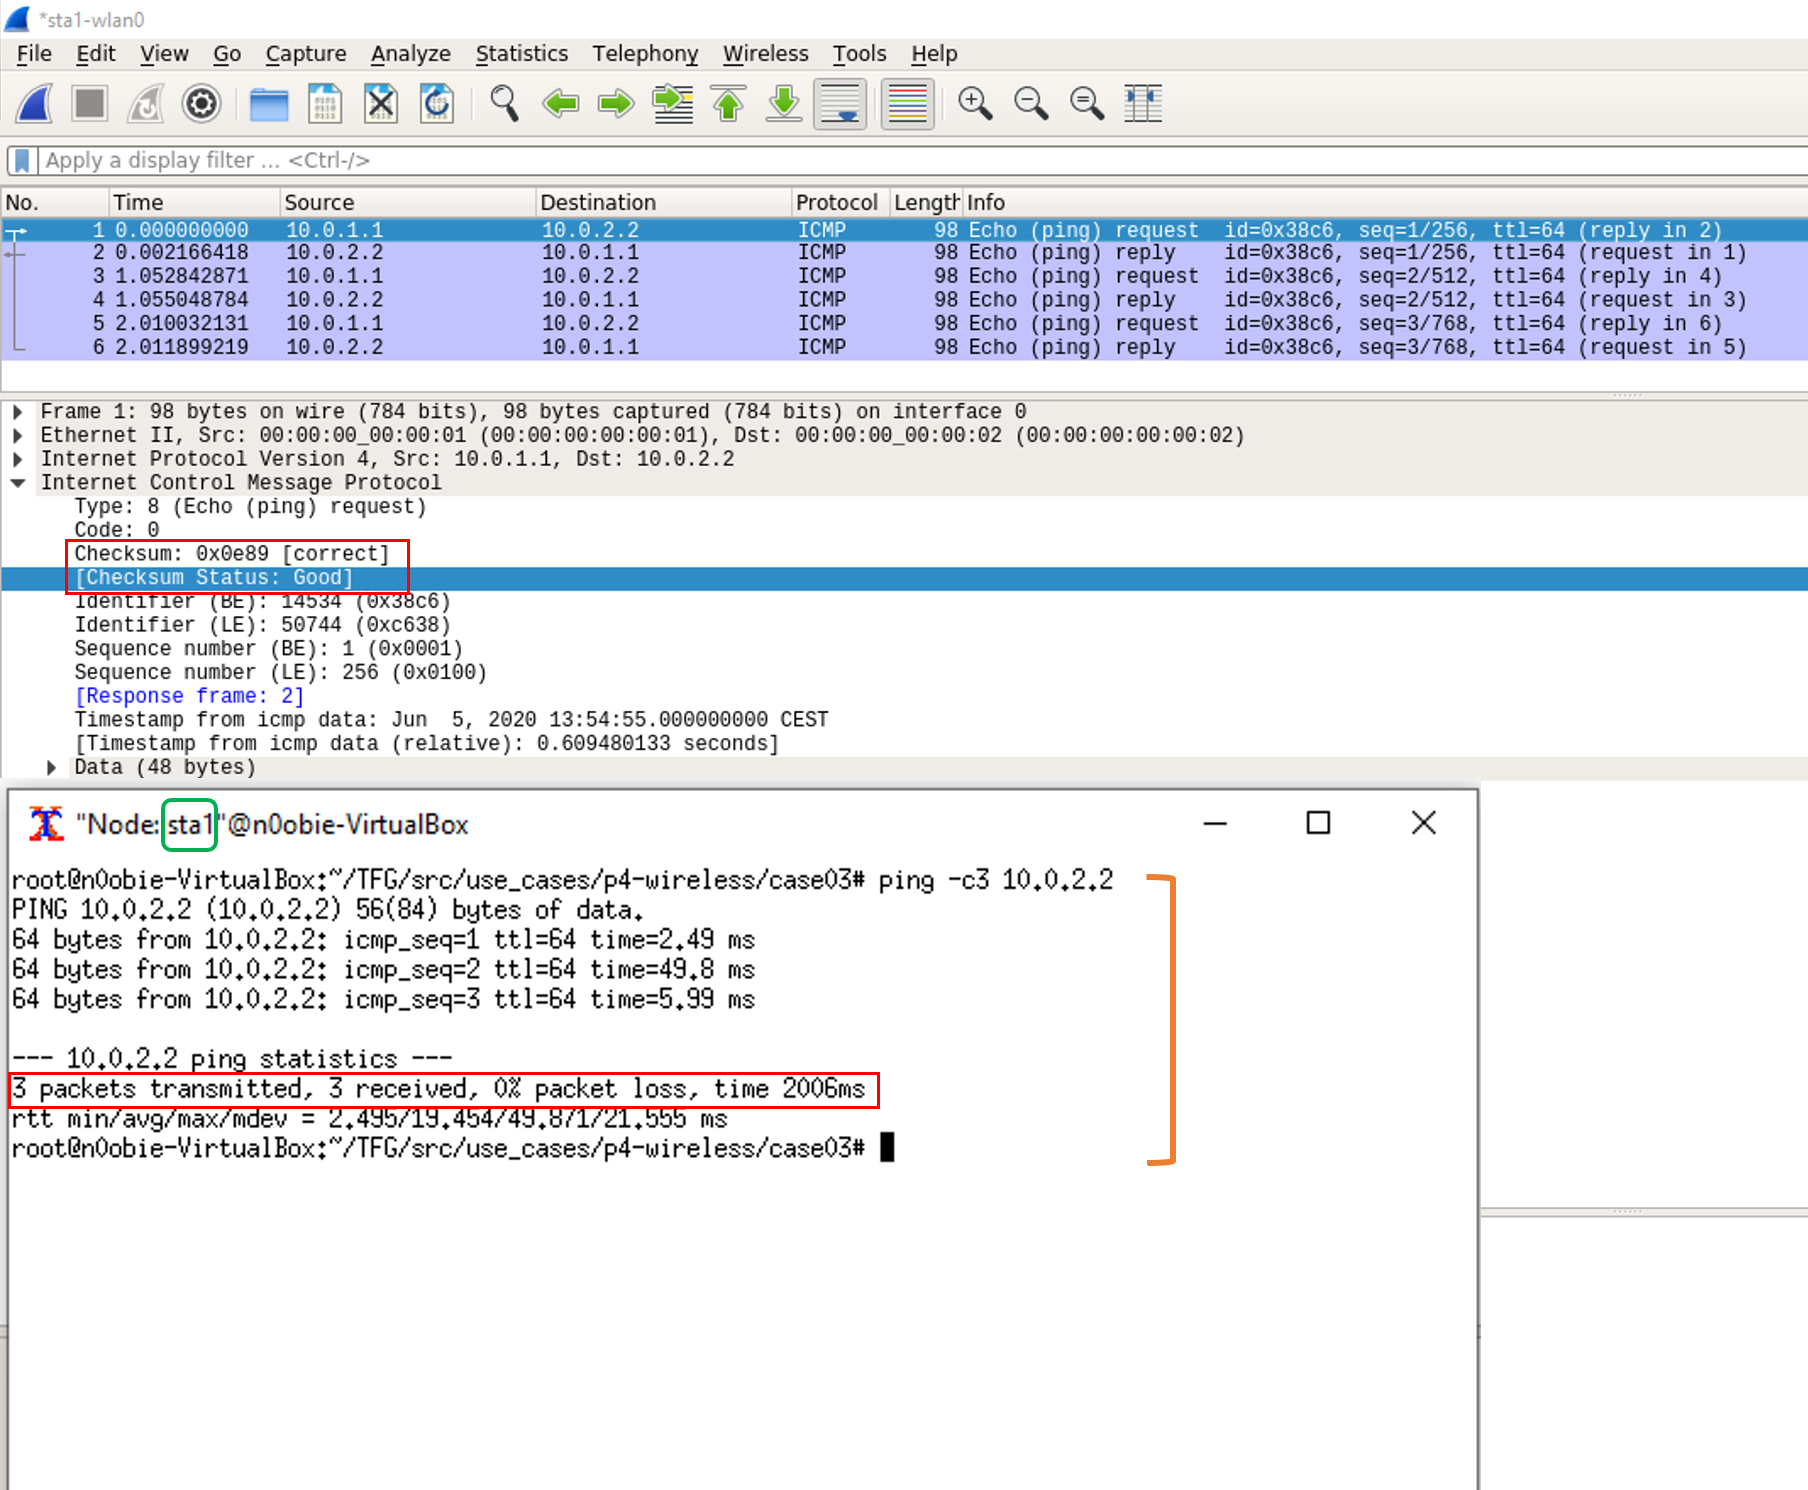
\includegraphics[width=14cm]{archivos/img/dev/p4-wifi/case03/demo_case03_edited.png}
    \caption{Comprobación de funcionamiento del Case03 - P4 Wireless}
    \label{fig:case03_p4_wifi_func1}
\end{figure}

\begin{lstlisting}[language= bash, style=Consola, caption={Pasos a seguir para comprobar el funcionamiento - Case03},label=code:case03_p4_wifi_func1]
    mininet-wifi>  xterm sta1
    
    # Se hará ping desde la estación Wifi al Host.
    [sta1] wireshark &
    [sta1] ping 10.0.2.2
\end{lstlisting}
\vspace{0.5cm}

Como se puede ver en la figura \ref{fig:case03_p4_wifi_func1}, todo funciona correctamente ya que se están recibiendo respuesta a los pings \fcolorbox{black}{orange}{\rule{0pt}{2.5pt}\rule{2.5pt}{0pt}}\hspace{1mm}. De forma adicional, se puede comprobar con Wireshark como el \textit{checksum} de la cabecera ICMP viene correctamente calculado.
\subsection{Case04 - Layer 3 forwarding}
\label{p4_wifi_case04}


 En este caso de uso trataremos de implementar un forwarding a nivel de red, capa 3, por ello nuestro hipotético "switch" será ahora un un router muy básico y con muy pocas funcionalidades. Al igual que en los casos de uso anteriores, se hará uso de software switch llamado \gls{bmv2}, para testear los programas P4, y de la integración desarrollada anteriormente con Mininet-WiFi como escenario para recrear las topologías de Red. En este caso también, el \gls{bmv2} será configurado vía P4Runtime  por lo que se hará uso de la clase de \texttt{P4RuntimeAP}. En el caso de querer configurar el \gls{bmv2} vía Thrift-port se podría utilizar la clase desarrollada \texttt{P4AP}.\\
\par

Dado que toda la información relativa a este caso de uso ya se ha explicado anteriormente en el case04 de P4 cableado (Ver subsección \ref{P4_ether_case04}), y no hay ninguna diferencia inducida en el cambio de entorno según se explico en las sección anterior,  únicamente se harán indicaciones sobre como poder compilarlo y ejecutarlo. Importante, si usted está replicando este caso de uso, sin antes haber adecuado las dependencias necesarias de Mininet-WiFi con soporte del \gls{bmv2}, vuelva a este punto \ref{mn_wifi_own_deps} y siga los pasos indicados.\\
\par

% figura escenario
\begin{figure}[ht]
    \centering
    \includegraphics[width=16cm]{archivos/img/dev/p4-wifi/case04/scenario.png}
    \caption{Escenario del Case04 - P4 Wireless}
    \label{fig:case04_p4_wifi_scenario}
\end{figure}



\vspace{0cm}
\textbf{Compilación}\\
\par

Para la compilación de este caso de uso, al igual que en los casos de uso anteriores se ha dejado preparado un Makefile, por tanto no es necesario que el usuario haga un uso directo del compilador p4c. Si se quiere saber más sobre como funciona el proceso de compilación, qué etapas hay, como se le "inyecta" el \texttt{json} generado al \gls{bmv2}, o qué distintos \textit{targets} hay en función de la arquitectura, le recomendamos que vuelva al case01 (\ref{p4_ether_case01}). Para llevar a cabo la compilación solo se tendrá que seguir los pasos indicados en el bloque \ref{code:case04_p4_wifi_load}.

\begin{lstlisting}[language= bash, style=Consola, caption={Compilación programa P4  - Case04},label=code:case04_p4_wifi_load]
    # Entramos al directorio 
    cd TFG/src/use_cases/p4-wireless/case04

    # Hacemos uso del Makefile
    sudo make
\end{lstlisting}
\vspace{0.5cm}


Una vez ejecutado el make, se habrá generado una estructura de directorios que se utilizarán en el lanzamiento del caso de uso. Bajo el directorio \texttt{build} se podrá encontrar el \texttt{json} generado por el compilador, será este \texttt{json} quien tenga toda la información requerida para conformar el \gls{bmv2}. Los directorios \texttt{log} y \texttt{pcap}, se utilizarán respectivamente para almacenar los logs del \gls{bmv2} y para guardar las capturas de paquetes de las interfaces asociadas a la instancia \gls{bmv2}. Comentar que la interfaz desarrollada admite opciones para no generar información de log, ni pcaps, se podrá configurar a medida desde el propio script que lanza el escenario.\\
\par



\vspace{0.2cm}
\textbf{Puesta en marcha del escenario}\\
\par

Al igual que en la compilación, se ha dejado preparado un script en Python para automatizar la puesta en marcha del escenario. Este script describe la topología que se utilizará en este caso de uso. Recordar que es necesario volver hacer un \texttt{make install} para instalar los módulos adicionales generados para la integración del \gls{bmv2} y Mininet-WiFi, además de tener instaladas las versiones indicadas en el análisis de la integración. Estas dependencias se pueden encontrar en el apartado \ref{mn_wifi_own_deps}. Una vez comprobado que posee todas la dependencias, simplemente se tendrá que ejecutar el script con el interprete de Python. Este script levantará la topología descrita en la figura \ref{fig:case04_p4_wifi_scenario}, compuesto por tres estaciones WiFi y por tres instancias del nodo \texttt{P4RuntimeAP}. Los nodos \texttt{apX}, del tipo \texttt{P4RuntimeAP}, tendrán tres interfaces, una wireless y dos par de \gls{veth} para comunicarse entre los distintos puntos de acceso.


\begin{lstlisting}[language= bash, style=Consola, caption={Puesta en marcha del escenario  - Case04},label=code:case04_p4_wifi_run]
    sudo python scenario.py
\end{lstlisting}


\vspace{0.5cm}
\textbf{Comprobación del funcionamiento}\\
\par


Tras las ejecución del script \texttt{scenario.py}, se tendría el escenario \ref{fig:case04_p4_wifi_scenario} levantado, y la CLI de Mininet-WiFi abierta. Para la comprobación de funcionamiento de este caso de uso, se van a seguir los mismos pasos que en el case05 (\ref{P4_ether_case05}) - P4 en un entorno alámbrico. Por tanto no se entrará hacer explicaciones que se creen redundantes, se indicarán los pasos seguidos para llevar a cabo la comprobación de funcionamiento y los resultados de dichas pruebas. 

\begin{lstlisting}[language= bash, style=Consola, caption={Pasos a seguir para comprobar el funcionamiento - Case04},label=code:case04_p4_wifi_func1]
    mininet-wifi>  pingall
\end{lstlisting}
\vspace{0.5cm}


% figura escenario
\begin{figure}[ht]
    \centering
    \includegraphics[width=10cm]{archivos/img/dev/p4-wifi/case04/demo_case04_edited.png}
    \caption{Comprobación de funcionamiento del Case04 - P4 Wireless}
    \label{fig:case04_p4_wifi_func1}
\end{figure}


Según se puede apreciar en la figura \ref{fig:case04_p4_wifi_func1}, hay perfecta conectividad entre todos los hosts de la topología. Además, se podría hacer uso de un \textit{sniffer} para comprobar que los paquetes llegan con el campo \texttt{ttl} modificado, en función de los saltos que ha dado el paquete. 
\subsection{Case05 - Broadcast}
\label{p4_wifi_case05}


En este test desarrollaremos un programa p4 que haga Broadcast. En este caso únicamente haremos Broadcast a nivel de enlace, capa 2. La motivación de este caso de uso es ver la diferencia de dificultad respecto del entorno XDP donde tuvimos que anclar de manera adicional un \textit{bytecode} e\gls{bpf} en el \gls{tc} además de propio programa \gls{xdp} anclado en la interfaz para lograr hacer un broadcast. Al igual que en los casos de uso anteriores, se hará uso de software switch llamado \gls{bmv2}, para testear los programas P4, y de la integración desarrollada anteriormente con Mininet-WiFi como escenario para recrear las topologías de Red.\\
\par


Dado que toda la información relativa a este caso de uso ya se ha explicado anteriormente en el case05 de P4 cableado (Ver subsección \ref{P4_ether_case05}), y no hay ninguna diferencia inducida en el cambio de entorno según se explico en las sección anterior,  únicamente se harán indicaciones sobre como poder compilarlo y ejecutarlo. Importante, como ya se ha indicado, si usted está replicando este caso de uso, sin antes haber adecuado las dependencias necesarias de Mininet-WiFi con soporte del \gls{bmv2}, vuelva a este punto \ref{mn_wifi_own_deps} y siga los pasos indicados.

% figura escenario
\begin{figure}[ht]
    \centering
    \includegraphics[width=16cm]{archivos/img/dev/p4-wifi/case05/scenario.png}
    \caption{Escenario del Case05 - P4 Wireless}
    \label{fig:case05_p4_wifi_scenario}
\end{figure}

\newpage

\vspace{0.2cm}
\textbf{Compilación}\\
\par

Para la compilación de este caso de uso, al igual que en los casos de uso anteriores se ha dejado preparado un Makefile, por tanto no es necesario que el usuario haga un uso directo del compilador p4c. Si se quiere saber más sobre como funciona el proceso de compilación, qué etapas hay, como se le "inyecta" el \texttt{json} generado al \gls{bmv2}, o qué distintos \textit{targets} hay en función de la arquitectura, le recomendamos que vuelva al case01 (\ref{p4_ether_case01}). Para llevar a cabo la compilación solo se tendrá que seguir los pasos indicados en el bloque \ref{code:case04_p4_wifi_load}.

\begin{lstlisting}[language= bash, style=Consola, caption={Compilación programa P4  - Case05},label=code:case05_p4_wifi_load]
    # Entramos al directorio 
    cd TFG/src/use_cases/p4-wireless/case05

    # Hacemos uso del Makefile
    sudo make
\end{lstlisting}
\vspace{0.5cm}


Una vez ejecutado el make, se habrá generado una estructura de directorios que se utilizarán en el lanzamiento del caso de uso. Bajo el directorio \texttt{build} se podrá encontrar el \texttt{json} generado por el compilador, será este \texttt{json} quien tenga toda la información requerida para conformar el \gls{bmv2}. Los directorios \texttt{log} y \texttt{pcap}, se utilizarán respectivamente para almacenar los logs del \gls{bmv2} y para guardar las capturas de paquetes de las interfaces asociadas a la instancia \gls{bmv2}.\\
\par



\vspace{0.2cm}
\textbf{Puesta en marcha del escenario}\\
\par

Al igual que en la compilación, se ha suministrado un script en Python para automatizar la puesta en marcha del escenario. Este script conformará la topología que se utilizará en este caso de uso. Se quiere recordar que es necesario volver hacer un \texttt{make install} para instalar los módulos adicionales generados para la integración del \gls{bmv2} y Mininet-WiFi, además de tener instaladas las versiones indicadas en el análisis de la integración. Estas dependencias se pueden encontrar en el apartado \ref{mn_wifi_own_deps} \\
\par

Una vez comprobadas la dependencias, simplemente se tendrá que ejecutar el script con el interprete de Python. Este script levantará la topología descrita en la figura \ref{fig:case05_p4_wifi_scenario}, compuesto por tres estaciones WiFi y por una instancia del nodo \texttt{P4RuntimeAP}. El nodo \texttt{ap1}, del tipo \texttt{P4RuntimeAP}, tendrá una interfaz,  del tipo wireless, con la cual se comunicará con todas las estaciones WiFi.



\begin{lstlisting}[language= bash, style=Consola, caption={Puesta en marcha del escenario  - Case05},label=code:case05_p4_wifi_run]
    sudo python scenario.py
\end{lstlisting}
\vspace{0.2cm}

\vspace{0.5cm}
\textbf{Comprobación del funcionamiento}\\
\par


Tras las ejecución del script \texttt{scenario.py}, se tendría el escenario \ref{fig:case05_p4_wifi_scenario} levantado, y la CLI de Mininet-WiFi abierta. Para la comprobación de funcionamiento de este caso de uso, se van a seguir los mismos pasos que en el case05 (\ref{P4_ether_case05}) - P4 en un entorno alámbrico. Por tanto no se entrará hacer explicaciones que se creen redundantes, se indicarán los pasos seguidos para llevar a cabo la comprobación de funcionamiento y los resultados de dichas pruebas. 

\begin{lstlisting}[language= bash, style=Consola, caption={Pasos a seguir para comprobar el funcionamiento - Case05},label=code:case05_p4_wifi_func1]
    mininet-wifi>  xterm sta1 sta2 sta3
    
    # Nos ponemos a escuchar en las estaciones wifi destino
    [sta2] tcpdump -l
    [sta3] tcpdump -l
    
    
    # Generamos ARP-Request desde sta1
    [sta1] arping 10.0.2.2
\end{lstlisting}
\vspace{0.5cm}


Como se puede apreciar en la figura \ref{fig:case05_p4_wifi_func1} el ARP-Request llega correctamente. Se ve como los paquetes ARP-Request están llegando tanto al \texttt{sta2} como a la \texttt{sta3}. Pero solo será la \texttt{sta2}, en este caso, la que contesta ya que va dirigido a ésta. \\
\par

Esto se debe a que al completarse la resolución ARP, la \texttt{sta1} ya conoce la dirección MAC de la \texttt{sta2}, por tanto los ARP-Request que se generen a posteriori llevarán la MAC destino la de la estación WiFi \texttt{sta2}, entonces el \gls{ap} no lo difundirá por todos su puertos, se lo pasará directamente a la \texttt{sta2}.

\newpage

\begin{figure}[h!]
    \centering
    \begin{subfigure}[b]{\textwidth}
    	\centering
        \includegraphics[width=8cm]{archivos/img/dev/p4-wifi/case05/demo_case05_1_edited.png}
        \caption{Ejecución de arping hacia la estación WiFi sta2}
        \label{fig:case05_p4_wifi_func_ping}
    \end{subfigure}
    \par\bigskip
    \begin{subfigure}[b]{\textwidth}
    	\centering
        \includegraphics[width=12cm]{archivos/img/dev/p4-wifi/case05/demo_case05_2_edited.png}
        \caption{Escucha con Tcpdump en la estación WiFi sta3}
        \label{fig:case05_p4_wifi_func_list1}
    \end{subfigure}
    \par\bigskip
    \begin{subfigure}[b]{\textwidth}
    	\centering
        \includegraphics[width=12cm]{archivos/img/dev/p4-wifi/case05/demo_case05_3_edited.png}
        \caption{Escucha con Tcpdump en la estación WiFi sta2}
        \label{fig:case05_p4_wifi_func_list2}
    \end{subfigure}
    
    \caption{Comprobación de funcionamiento del Case05 - P4 Wireless}
    \label{fig:case05_p4_wifi_func1}
\end{figure}


%%%%%%%%%%%%%%%%%%%%%%%%%%%%%%%%%%%%%%%%%%%%%%%%%%%%%%%%%%%%%%%%%%%%%%%%%%%%%%%%%%%%%%%%
\section{Casos de uso \glsentryshort{xdp} en medios inalámbricos}

En esta sección se introducirán todos los casos de uso realizados con la tecnología \gls{xdp} en entornos inalámbricos. Todos los casos de uso se han nombrado siguiendo la misma sintaxis que en el repositorio del \gls{tfg}, alojado en GitHub. Para \textbf{la instalación de las dependencias} de la tecnología \gls{xdp} se ha dejado escrito el Anexo \ref{deps}, donde se detallan todos los pasos a seguir. De forma adicional, y como se comentó en el capítulo \ref{analisisPreimplementacion}, se hará uso de Mininet-WiFi como plataforma para probar los casos de uso desarrollados en un entorno inalámbrico.\\
\par

Los casos de uso se han dividido en cinco partes, con la finalidad de que la lectura de estos sea más clara y ordenada.

\begin{itemize}
    \item \textbf{Introducción}: En esta parte se abordará las explicaciones teóricas complementarias en caso de que sean necesario, muchas de ellas se habrán dado ya en los casos de uso \gls{xdp} en entornos cableados, por lo que se referenciará a dichas explicaciones.
    
    \item \textbf{Compilación}: En esta parte se explicará al lector cómo proceder para compilar el programa \gls{xdp}.
    
    \item \textbf{Puesta en marcha del escenario}: En esta parte se explicará al lector cómo levantar el escenario y cómo poder limpiarlo tras finalizar la comprobación de funcionamiento.
    \item \textbf{Carga de los programas \gls{xdp}}, en esta parte se indicará sobre qué interfaz se producirá la carga de los programas \gls{xdp}, y se ha realizado dicha carga, ya que se hará de forma automática en el script que levanta el escenario.
    
    \item \textbf{Evaluación del funcionamiento}: Por último se hará una evaluación sobre el funcionamiento del caso de uso.
\end{itemize}

\vspace{1cm}

Para que el lector pueda seguir el desarrollo con los casos de uso, a continuación se indica la tabla \ref{tab:XDP_wifi_usecases}, la cual expone en qué ruta del repositorio del \gls{tfg} se puede encontrar dicho caso de uso, y un vídeo demostración donde el autor va comentando paso a paso el caso de uso y su evaluación. 

\begin{table}[ht]
\centering
\resizebox{\textwidth}{!}{%
\begin{tabular}{|l|c|c|}
\hline
\rowcolor[HTML]{EFEFEF} 
\multicolumn{1}{|c|}{\cellcolor[HTML]{EFEFEF}\textbf{Caso de uso}} & \textbf{Enlace al repositorio} & \textbf{Enlace al vídeo demostración  } \\ \hline
case01 - Drop                                                      & \href{https://github.com/davidcawork/TFG/tree/master/src/use_cases/xdp-wireless/case01}{\texttt{Enlace al código}}                         & \href{https://youtu.be/7v-Fsw43Zew}{Enlace al vídeo}                                \\ \hline
case02 - Pass                                                      & \href{https://github.com/davidcawork/TFG/tree/master/src/use_cases/xdp-wireless/case02}{\texttt{Enlace al código}}                         & \href{https://youtu.be/8ua-d7t0d_M}{Enlace al vídeo}                                \\ \hline
case03 - Echo server                                               & \href{https://github.com/davidcawork/TFG/tree/master/src/use_cases/xdp-wireless/case03}{\texttt{Enlace al código}}                          & \href{https://youtu.be/02zlWZM_mEk}{Enlace al vídeo}                                \\ \hline
case04 - Layer 3 forwarding                                        & \href{https://github.com/davidcawork/TFG/tree/master/src/use_cases/xdp-wireless/case04}{\texttt{Enlace al código}}                           & \href{https://youtu.be/QL9lTdYmQ8s}{Enlace al vídeo}                                \\ \hline
case05 - Broadcast                                                 & \href{https://github.com/davidcawork/TFG/tree/master/src/use_cases/xdp-wireless/case05}{\texttt{Enlace al código}}                          & \href{https://youtu.be/hNnrkMMN3W8}{Enlace al vídeo}                                \\ \hline
\end{tabular}
}
\caption{Resumen de la documentación sobre los casos de uso XDP en entornos inalámbricos}
\label{tab:XDP_wifi_usecases}
\end{table}

\newpage

%%%%%%%%%%%%%%%%%%%%%%%%%%%%%%%%%%%%%%%%%%%%%%%%%%%%%%%%%%%%%%%%%%%%%%%%%%%%%%%%%%%%%%%%%%%%%%%
%   Casos de uso XDP medio Cableados 
\subsection{Case01 - Drop}
\label{xdp_wifi_case01}

En este caso de uso se probará que es posible descartar todos los paquetes recibidos haciendo uso de la tecnología XDP en un entorno inalámbrico. Para la realizar la prueba, primero se debe compilar el programa XDP y segundo levantar el escenario donde se va a realizar la prueba  de funcionamiento. En el proceso del levantamiento de la topología en Mininet-WiFi se anclará el binario a un interfaz del escenario, por lo que únicamente se tendrá que preocupar de observar los resultados cuando se genere tráfico que atraviese dicha interfaz.\\
\par
\vspace{0.5cm}
\textbf{Compilación}\\
\par

Para compilar el programa \gls{xdp} se ha dejado un Makefile preparado en este directorio al igual que en los casos de uso \gls{xdp} en entornos cableados. Por lo tanto, para compilarlo únicamente hay que seguir las indicaciones del bloque \ref{code:case01_xdp_wifi_compilacion}.

\begin{lstlisting}[language= bash, style=Consola, caption={Compilación programa XDP - Case01},label=code:case01_xdp_wifi_compilacion]
    # En caso de no haber entrado en el directorio asignado del caso de uso
    cd TFG/src/use_cases/xdp-wireless/case01
    
    
    # Hacemos uso del Makefile suministrado 
    sudo make
\end{lstlisting}
\vspace{0.5cm}

Si tiene dudas sobre el proceso de compilación del programa \gls{xdp} le recomendamos que vuelva al case02 (\gls{xdp} - Cableado \ref{xdp_ether_case02}) donde se hace referencia al \textit{flow} dispuesto para la compilación de los programas \gls{xdp}.



\vspace{1cm}
\textbf{Puesta en marcha del escenario}\\
\par

Para testear los programas \gls{xdp} en un entorno inalámbrico, se hará uso de Mininet-WiFi para emular las topologías de red. Para levantar el escenario solo se tendrá que ejecutar el script en Python que hace uso de la API de Mininet-WiFi para generar toda la topología de red. Una vez ejecutado este abrirá la interfaz de linea de comandos de Mininet-WiFi, desde la cual se podrá comprobar el funcionamiento del caso de uso. En este caso, se realiza la carga del programa \gls{xdp} desde el propio script de Python, haciendo uso de la herramienta xdp\_loader desarrollada para ello. Por tanto, como se ha dicho este script está auto-contenido, por lo que solo se deberá ejecutarlo. \\
\par

Para limpiar la máquina del escenario recreado anteriormente con Mininet-WiFi se podría realizar un \texttt{sudo mn -c}, pero se recomienda al usuario que haga uso del \textit{target} del Makefile destinado para ello, ya que adicionalmente limpiará los ficheros intermedios generados en el proceso de compilación de nuestro programa \gls{xdp}. Ejecutando el siguiente comando se limpiaría la máquina.

\begin{lstlisting}[language= bash, style=Consola, caption={Compilación programa XDP - Case01},label=code:case01_xdp_wifi_run]
    # Levantamos el escenario
    sudo python runenv.py
    
    
    # Limpiamos el escenario
    sudo make clean
\end{lstlisting}
\vspace{0.5cm}

Por último, únicamente indicar que el escenario recreado es el siguiente, compuesto exclusivamente de dos estaciones \textit{wireless}, aisladas en sus propias \textit{Network Namespaces}, y un punto de acceso corriendo el \textit{daemon} de HostApd para intercomunicar dichas estaciones WiFi.

% figura escenario
\begin{figure}[ht]
    \centering
    \includegraphics[width=16cm]{archivos/img/dev/xdp-wifi/case01/scenario.png}
    \caption{Escenario inalámbrico del Case01 - XDP}
    \label{fig:case01_xdp_wifi_scenario}
\end{figure}

\vspace{0.5cm}
\textbf{Carga del programa XDP}\\
\par

Como ya se ha comentado, la carga del programa \gls{xdp}, se llevará a cabo en el proceso del levantamiento del escenario, descrito en el script de Python para crear la topología. La carga del programa \gls{xdp}, se hará con el programa \texttt{xdp\_loader}, utilizado anteriormente para cargar los programas \gls{xdp} en interfaces alámbricas. 

\begin{lstlisting}[language= bash, style=Consola, caption={Carga del programa XDP - Case01},label=code:case01_xdp_wifi_load]
    # Linea 38 del script runenv.py
    sta1.cmd("./xdp_loader -S -d sta1-wlan0 -F --progsec xdp_case01")
\end{lstlisting}
\newpage
Es importante señalar, que el comando ejecutado dentro de la \textit{Network Namespace} de la estación WiFi \texttt{sta1}, no se ha lanzado con permisos de root, ya que esta orden los heredará al lanzar el script que levanta la topología en Mininet-WiFi. 

\vspace{1cm}
\textbf{Comprobación del funcionamiento}\\
\par

Una vez que el programa \gls{xdp} fue anclado a la interfaz de la estación WiFi \texttt{sta1}, es necesario comprobar si realmente funciona según lo esperado, y ver si las interfaces generadas por el módulo mac80211\_hwsim son compatibles con \gls{xdp}. Esto se hará generando tráfico desde una estación WiFi hacia la otra, para que atraviese por la interfaz que tiene anclado el programa \gls{xdp}. En este caso el comportamiento esperado es que haga un \textit{drop} de los paquetes nada más llegar a la interfaz, en este caso la interfaz \texttt{sta1-wlan0}.\\
\par
Como en anteriores casos de uso, se ha habilitado la recolección de estadísticas sobre los códigos de retorno \gls{xdp}, por lo que sería una buena práctica comprobar si se están empleando códigos de retorno \texttt{XDP\_DROP}.


% figura escenario
\begin{figure}[ht]
    \centering
    \includegraphics[width=14cm]{archivos/img/dev/xdp-wifi/case01/demo_case01_edited.png}
    \caption{Comprobación de funcionamiento del Case01 - XDP Wireless}
    \label{fig:case01_xdp_wifi_func}
\end{figure}

Como se puede apreciar en la figura \ref{fig:case01_xdp_wifi_func}, inicialmente se realiza un ping \fcolorbox{black}{orange}{\rule{0pt}{2.5pt}\rule{2.5pt}{0pt}}\hspace{1mm} entre las estaciones WiFi, pero no hay conectividad debido a que el programa \gls{xdp} está tirando los paquetes. Acto seguido se quita el programa \gls{xdp} de la interfaz y se vuelve a probar la conectividad entre las estaciones WiFi ejecutando un segundo ping \fcolorbox{black}{green}{\rule{0pt}{2.5pt}\rule{2.5pt}{0pt}}\hspace{1mm}. Se ve que una vez desanclado el programa, la conectividad vuelve, por lo que se puede afirmar que el funcionamiento es el esperado.  
\subsection{Case02 - Pass}
\label{xdp_wifi_case02}

En este caso de uso se probará que es posible admitir todos los paquetes recibidos haciendo uso de la tecnología \gls{xdp} en un entorno inalámbrico. ¿Qué significa ``Admitir”? se quiere comprobar si es posible dejar pasar los paquetes, sin afectarles el plano de datos programado con la tecnología, ya que, aunque \gls{xdp} mucha gente lo concibe para hacer un \textit{by-pass} al \textit{stack} de red del Kernel de Linux, una completa redefinición del mismo, en muchas ocasiones será útil trabajar en conjunto para conseguir la funcionalidad deseada. En este caso, además se verá si existe alguna diferencia inducida por el cambio de entorno, de alámbrico a \textit{wireless}.\\
\par


\vspace{0.5cm}
\textbf{Compilación}\\
\par

Para compilar el programa \gls{xdp}, al igual que en casos de uso anteriores, se ha dejado un Makefile preparado en este directorio. Por lo tanto, para compilarlo únicamente hay que seguir las indicaciones del bloque \ref{code:case02_xdp_wifi_compilacion}.\\
\par

\begin{lstlisting}[language= bash, style=Consola, caption={Compilación programa XDP - Case02},label=code:case02_xdp_wifi_compilacion]
    # En caso de no haber entrado en el directorio asignado del caso de uso
    cd TFG/src/use_cases/xdp-wireless/case02
    
    
    # Hacemos uso del Makefile suministrado 
    sudo make
\end{lstlisting}
\vspace{0.5cm}

Si tiene dudas sobre el proceso de compilación del programa \gls{xdp} le recomendamos que vuelva al case02 (\gls{xdp} - Cableado \ref{xdp_ether_case02}) donde se hace referencia al \textit{flow} dispuesto para la compilación de los programas \gls{xdp}.\\
\par



\vspace{1cm}
\textbf{Puesta en marcha del escenario}\\
\par

Para testear los programas \gls{xdp} en un entorno inalámbrico, se hará uso de Mininet-WiFi para emular las topologías de red. Para levantar el escenario solo se tendrá que ejecutar el script en Python que hace uso de la API de Mininet-WiFi para generar toda la topología de red. Una vez ejecutado este abrirá la interfaz de linea de comandos de Mininet-WiFi, desde la cual se podrá comprobar el funcionamiento del caso de uso. En este caso, se realiza la carga del programa \gls{xdp} desde el propio script de Python, haciendo uso de la herramienta xdp\_loader desarrollada para ello. Por tanto, como se ha dicho este script está auto-contenido, por lo que solo se deberá ejecutarlo. \\
\par

Para limpiar la máquina del escenario recreado anteriormente con Mininet-WiFi se podría realizar un \texttt{sudo mn -c}, pero se recomienda al usuario que haga uso del \textit{target} del Makefile destinado para ello, ya que adicionalmente limpiará los ficheros intermedios generados en el proceso de compilación de nuestro programa \gls{xdp}. Ejecutando el siguiente comando se limpiaría la máquina.\\
\par

\begin{lstlisting}[language= bash, style=Consola, caption={Compilación programa XDP - Case02},label=code:case02_xdp_wifi_run]
    # Levantamos el escenario
    sudo python runenv.py
    
    
    # Limpiamos el escenario
    sudo make clean
\end{lstlisting}
\vspace{0.5cm}


Por último, únicamente indicar que el escenario recreado es el siguiente, compuesto exclusivamente de dos estaciones \textit{wireless}, aisladas en sus propias \textit{Network Namespaces}, y un punto de acceso corriendo el \textit{daemon} de HostApd para intercomunicar dichas estaciones WiFi.\\
\par

% figura escenario
\begin{figure}[ht]
    \centering
    \includegraphics[width=16cm]{archivos/img/dev/xdp-wifi/case02/scenario.png}
    \caption{Escenario inalámbrico del Case02 - XDP}
    \label{fig:case02_xdp_wifi_scenario}
\end{figure}


\vspace{0.5cm}
\textbf{Carga del programa XDP}\\
\par
Como ya se ha comentado, la carga del programa \gls{xdp}, se llevará a cabo en el proceso del levantamiento del escenario, descrito en el script de Python para crear la topología. La carga del programa \gls{xdp}, se hará con el programa \texttt{xdp\_loader}, utilizado anteriormente para cargar los programas \gls{xdp} en interfaces alámbricas. \\
\par

\begin{lstlisting}[language= bash, style=Consola, caption={Carga del programa XDP - Case02},label=code:case02_xdp_wifi_load]
    # Linea 37 del script runenv.py
    sta1.cmd("./xdp_loader -S -d sta1-wlan0 -F --progsec xdp_case02")
\end{lstlisting}
\vspace{0.5cm}
En estos primeros casos de uso \gls{xdp} en un entorno inalámbrico, la carga de los programas se está realizando en el propio script que levanta la topología en Mininet-WiFi, pero más adelante en el case04 (Ir a subsección \ref{xdp_wifi_case04}) se verá como se puede ejecutar comandos dentro de la \textit{Network Namespace} indicada para lograr la carga de un programa \gls{xdp} en una interfaz de un nodo independiente de la red desde la propia CLI de Mininet-WiFi.\\
\par



\vspace{0.5cm}
\textbf{Comprobación del funcionamiento}\\
\par

Una vez que el programa \gls{xdp} fue anclado a la interfaz de la estación WiFi \texttt{sta1}, es necesario asegurarse de que funciona según lo esperado, y ver si el funcionamiento obtenido difiere al funcionamiento de este mismo caso de uso en un medio cableado.  La prueba que se va a realizar puede que sea un poco simple, pero es válida, ya que únicamente queremos verificar que el programa anclado en la interfaz está delegando los paquetes que le llegan al \textit{stack} de red.\\
\par



\begin{lstlisting}[language= bash, style=Consola, caption={Comprobación del funcionamiento - Case02},label=code:case02_xdp_wifi_func1]
    # Hacemos ping desde una estación wifi hacia la otra. Deberíamos tener conectividad.
    mininet-wifi> sta2 ping sta1
    
    # Comprobamos los códigos de retorno XDP
    mininet-wifi> sta1 ./xdp_stats -d sta1-wlan0
\end{lstlisting}

% figura escenario
\begin{figure}[ht]
    \centering
    \includegraphics[width=12cm]{archivos/img/dev/xdp-wifi/case02/demo_case02_1_edited.png}
    \caption{Comprobación de funcionamiento (Ping) del Case02 - XDP Wireless}
    \label{fig:case02_xdp_wifi_func1}
\end{figure}
\newpage
% figura escenario
\begin{figure}[ht!]
    \centering
    \includegraphics[width=14cm]{archivos/img/dev/xdp-wifi/case02/demo_case02_2_edited.png}
    \caption{Comprobación de funcionamiento (Stats) del Case02 - XDP Wireless}
    \label{fig:case02_xdp_wifi_func2}
\end{figure}

Según se puede ver en la figura \ref{fig:case02_xdp_wifi_func1}, hay perfecta conectividad entre las estaciones WiFi dado que el ping \fcolorbox{black}{green}{\rule{0pt}{2.5pt}\rule{2.5pt}{0pt}}\hspace{1mm} está funcionando correctamente. Por lo que, se presupone que el programa \gls{xdp} está dejando pasar los paquetes ICMP hacia el \textit{stack} de red. Apreciando la figura \ref{fig:case02_xdp_wifi_func1}, dicha presuposición se confirma, atendiendo al contador de los códigos de retorno \texttt{XDP\_PASS}. 
\subsection{Case03 - Echo server}
\label{xdp_wifi_case03}

En este caso de uso se explorará el análisis de paquetes, su filtrado y manejo. En los anteriores caso de uso exclusivamente se definía un comportamiento de los paquetes haciendo un uso exclusivo de los códigos de retorno \gls{xdp}, más concretamente \texttt{XDP\_DROP} para tirar los paquetes y \texttt{XDP\_PASS} para admitir los paquetes.\\
\par
Por tanto, en este test se filtrarán los paquetes por sus cabeceras, haciendo uso de las estructuras indicadas en este mismo caso de uso en un entorno cableado (Ir a \ref{xdp_ether_case03}). Se filtrarán los paquetes ICMP con el código \texttt{ECHO-Request}, se modificarán sus campos para conformar su respuesta, y se reenviará dicho paquete a la misma interfaz por la cual llegó para que sea entregado a su emisor. De esta forma se conformará un servidor de Echo, que responderá a todos los pings que lleguen a la interfaz que tenga cargado este programa \gls{xdp}. 

\vspace{0.5cm}
\textbf{Compilación}\\
\par

Para compilar el programa \gls{xdp}, al igual que en casos de uso anteriores, se ha dejado un Makefile preparado en este directorio. Por lo tanto, para compilarlo únicamente hay que seguir las indicaciones del bloque \ref{code:case03_xdp_wifi_compilacion}.

\begin{lstlisting}[language= bash, style=Consola, caption={Compilación programa XDP - Case03},label=code:case03_xdp_wifi_compilacion]
    # En caso de no haber entrado en el directorio asignado del caso de uso
    cd TFG/src/use_cases/xdp-wireless/case03
    
    
    # Hacemos uso del Makefile suministrado 
    sudo make
\end{lstlisting}
\vspace{0.5cm}

Si tiene dudas sobre el proceso de compilación del programa \gls{xdp} le recomendamos que vuelva al case02 (\gls{xdp} - Cableado \ref{xdp_ether_case02}) donde se hace referencia al \textit{flow} dispuesto para la compilación de los programas \gls{xdp}.\\
\par



\vspace{0.5cm}
\textbf{Puesta en marcha del escenario}\\
\par

Para testear los programas \gls{xdp} en un entorno inalámbrico, se hará uso de Mininet-WiFi para emular las topologías de red. Para levantar el escenario solo se tendrá que ejecutar el script en Python que hace uso de la API de Mininet-WiFi para generar toda la topología de red. Una vez ejecutado este abrirá la interfaz de linea de comandos de Mininet-WiFi, desde la cual se podrá comprobar el funcionamiento del caso de uso. En este caso, se realiza la carga del programa XDP desde el propio script de Python, haciendo uso de la herramienta xdp\_loader desarrollada para ello. \\
\par

Para limpiar la máquina del escenario recreado anteriormente con Mininet-WiFi se podría realizar un \texttt{sudo mn -c}, pero se recomienda al usuario que haga uso del \textit{target} del Makefile destinado para ello, ya que adicionalmente limpiará los ficheros intermedios generados en el proceso de compilación de nuestro programa \gls{xdp}. Ejecutando el siguiente comando se limpiaría la máquina.
\newpage
\begin{lstlisting}[language= bash, style=Consola, caption={Compilación programa XDP - Case03},label=code:case03_xdp_wifi_run]
    # Levantamos el escenario
    sudo python runenv.py
    
    
    # Limpiamos el escenario
    sudo make clean
\end{lstlisting}
\vspace{0.7cm}


Por último, únicamente indicar que el escenario recreado es el siguiente, compuesto exclusivamente de dos estaciones \textit{wireless}, aisladas en sus propias \textit{Network Namespaces}, y un punto de acceso corriendo el \textit{daemon} de HostApd para intercomunicar dichas estaciones WiFi.\\
\par

% figura escenario
\begin{figure}[ht]
    \centering
    \includegraphics[width=16cm]{archivos/img/dev/xdp-wifi/case03/scenario.png}
    \caption{Escenario inalámbrico del Case03 - XDP}
    \label{fig:case03_xdp_wifi_scenario}
\end{figure}


\vspace{0.6cm}
\textbf{Carga del programa XDP}\\
\par
Como ya se ha comentado, la carga del programa \gls{xdp}, se llevará a cabo en el proceso del levantamiento del escenario, descrito en el script de Python para crear la topología. La carga del programa \gls{xdp}, se hará con el programa \texttt{xdp\_loader}, utilizado anteriormente para cargar los programas \gls{xdp} en interfaces alámbricas. 

\newpage

\begin{lstlisting}[language= bash, style=Consola, caption={Carga del programa XDP - Case03},label=code:case03_xdp_wifi_load]
    # Linea 37 del script runenv.py
    ap1.cmd("./xdp_loader -S -d ap1-wlan1 -F --progsec xdp_case03")
\end{lstlisting}
\vspace{0.5cm}
En este caso, se puede apreciar como la carga del programa \gls{xdp} se está llevando a cabo sobre la interfaz del punto de acceso \texttt{ap1}. Dado que únicamente son los paquetes ICMP los que serán interceptados y contestados, los paquetes de control del punto de acceso no se verán afectados, irán directamente al \textit{daemon} HostApd haciendo uso del código de retorno \texttt{XDP\_PASS}.\\
\par


\vspace{0.5cm}
\textbf{Comprobación del funcionamiento}\\
\par

La comprobación del funcionamiento del programa \gls{xdp} anclado a la interfaz \texttt{ap1-wlan1} se llevará a cabo generando pings desde las estaciones wireless hacia el punto de acceso, para que la interfaz \texttt{ap1-wlan1} los filtre, analice y nos genere una respuesta. Si todo funciona correctamente deberíamos ver como los códigos de retorno mayormente empleados son los de \texttt{XDP\_TX} siempre y cuando no hayamos detenido el ping desde dentro de la \textit{Network Namespace}. 


\begin{lstlisting}[language= bash, style=Consola, caption={Comprobación del funcionamiento - Case03},label=code:case03_xdp_wifi_func1]
    # Lanzamos un ping desde una estación wireless hacia cualquier máquina
    mininet-wifi> sta1 ping 9.9.9.9
    
    # En una consola aparte lanzamos el programa xdp_stats para ir viendo a tiempo real
    # los códigos de retorno XDP empleados
    mininet-wifi> ap1 ./xdp_stats -d ap1-wlan1
\end{lstlisting}

% figura escenario
\begin{figure}[ht!]
    \centering
    \includegraphics[width=12cm]{archivos/img/dev/xdp-wifi/case03/demo_case03_1_edited.png}
    \caption{Comprobación de funcionamiento (Ping) del Case03 - XDP Wireless}
    \label{fig:case03_xdp_wifi_func1}
\end{figure}

Como se puede ver en la figura \ref{fig:case03_xdp_wifi_func1}, se está realizando ping hacia una máquina inexistente, pero como en el script de aprovisionamiento se le han indicado a todas las estaciones WiFi un hipotético \textit{gateway}, y se ha añadido en la tabla ARP la MAC de ese hipotético \textit{gateway}, no habrá una resolución ARP previa al envío del ping. Por tanto se generará el ping \fcolorbox{black}{orange}{\rule{0pt}{2.5pt}\rule{2.5pt}{0pt}}\hspace{1mm}, que llegará a la interfaz la cual tiene cargado el programa \gls{xdp}, y como se puede apreciar en la figura \ref{fig:case03_xdp_wifi_func2}, dichos pings \fcolorbox{black}{orange}{\rule{0pt}{2.5pt}\rule{2.5pt}{0pt}}\hspace{1mm} son contestados correctamente por el programa devolviendo códigos de retorno \texttt{XDP\_TX}.

% figura escenario
\begin{figure}[ht!]
    \centering
    \includegraphics[width=15.5cm]{archivos/img/dev/xdp-wifi/case03/demo_case03_2_edited.png}
    \caption{Comprobación de funcionamiento (Stats) del Case03 - XDP Wireless}
    \label{fig:case03_xdp_wifi_func2}
\end{figure}


\subsection{Case04 - Layer 3 forwarding	}
\label{xdp_wifi_case04}

En este caso de uso se explorará el forwarding de paquetes, en este punto ya se debe conocer como filtrar por las cabeceras de los paquetes, analizarlos y establecer una lógica asociada a ese filtrado con los códigos de retorno \gls{xdp}. La gran diferencia en este entorno inalámbrico es el número de interfaces que suele tener un dispositivo \textit{wireless}. Generalmente en entornos cableados, un nodo suele tener tantas interfaces Ethernet como enlaces tenga con otros nodos, en cambio, en entornos wireless, con una misma interfaz puede tener enlaces con otros nodos siempre y cuando se encuentren en rango.\\
\par
Por tanto, los programas \gls{xdp} en entornos inalámbricos podrían realizar todo su forwarding haciendo uso de un único código de retorno \gls{xdp}, \texttt{XDP\_TX}. Con dicho código se reenviarían los paquetes recibidos a la interfaz a la cual llegaron los paquetes. Dado que en los entornos cableados, se tuvieron que hacer uso de los \textit{helpers} \gls{bpf} indicados en el bloque \ref{code:case04_xdp_ether_kernprog1}, se van a plantear escenarios similares donde sea necesario hacer un forwarding de una interfaz A a otra B. De esta forma, se verificará que dichas funciones siguen operativas en interfaces creadas con el módulo mac80211\_hwsim.\\
\par
No se ha querido plantear este caso de uso haciendo solo uso  del código de retorno \texttt{XDP\_TX}, ya que en el case03 \gls{xdp} \textit{Wireless} (Ir a \ref{xdp_wifi_case03}),  ya se hizo uso de este código y se vio que funcionaba correctamente, por lo que se entendía que era preferible explorar los \textit{helpers} \gls{bpf} en entornos inalámbricos.
 


\vspace{0.5cm}
\textbf{Compilación}\\
\par

Para compilar el programa \gls{xdp}, al igual que en casos de uso anteriores, se ha dejado un Makefile preparado en este directorio. Por lo tanto, para compilarlo únicamente hay que seguir las indicaciones del bloque \ref{code:case04_xdp_wifi_compilacion}.

\begin{lstlisting}[language= bash, style=Consola, caption={Compilación programa XDP - Case04},label=code:case04_xdp_wifi_compilacion]
    # En caso de no haber entrado en el directorio asignado del caso de uso
    cd TFG/src/use_cases/xdp-wireless/case04
    
    
    # Hacemos uso del Makefile suministrado 
    sudo make
\end{lstlisting}
\vspace{0.5cm}

Si tiene dudas sobre el proceso de compilación del programa \gls{xdp} le recomendamos que vuelva al case02 (\gls{xdp} - Cableado \ref{xdp_ether_case02}) donde se hace referencia al \textit{flow} dispuesto para la compilación de los programas \gls{xdp}.\\
\par



\vspace{0.5cm}
\textbf{Puesta en marcha del escenario}\\
\par

Para testear los programas \gls{xdp} en un entorno inalámbrico, se hará uso de Mininet-WiFi para emular las topologías de red. Para levantar el escenario solo se tendrá que ejecutar el script en Python que hace uso de la API de Mininet-WiFi para generar toda la topología de red. Una vez ejecutado este abrirá la interfaz de linea de comandos de Mininet-WiFi, desde la cual se podrá comprobar el funcionamiento del caso de uso. \\
\par

Para limpiar la máquina del escenario recreado anteriormente con Mininet-WiFi se podría realizar un \texttt{sudo mn -c}, pero se recomienda al usuario que haga uso del \textit{target} del Makefile destinado para ello, ya que adicionalmente limpiará los ficheros intermedios generados en el proceso de compilación de nuestro programa \gls{xdp}. Ejecutando el siguiente comando se limpiaría la máquina.

\begin{lstlisting}[language= bash, style=Consola, caption={Compilación programa XDP - Case04},label=code:case04_xdp_wifi_run]
    # Levantamos el escenario
    sudo python runenv.py
      
    # Limpiamos el escenario
    sudo make clean
\end{lstlisting}
\vspace{0.5cm}

%%%%%%%%%%%%%%%%%%%%%%%%%%%%%%%%%%%%%%%%%%%%%%%%%%%%%%%%%%%%%%%%%%%%%%%%%%%%%%%%%%%%
\subsubsection{Hardcoded forwarding}
\label{xdp_wifi_case04_hard}

La primera forma de implementación del forwarding es lo que denominaremos como Hardcoded forwarding. Como ya se comentó, es necesario hardcodear información de forwarding en el propio programa \gls{xdp}. El escenario levantado (Ver figura \ref{fig:case04_xdp_wifi_scenario}), está compuesto de una estación wireless y un host, que corren dentro de su respectivas \textit{Network Namespaces}, y un punto de acceso corriendo un proceso de HostApd para comunicar las dos estaciones wireless entre sí. De forma adicional, y por consistencia del caso de uso, se ha decidido correr dicho switch dentro de su propia \textit{Network Namespace} para que no haya lugar a dudas de que el forwarding se está realizando correctamente y no está habiendo \textit{by-passes} de ningún tipo. En este caso el forwarding lo haremos desde la interfaz \texttt{ap1-wlan1} hacia la interfaz \texttt{ap1-eth2}.\\
\par

% figura escenario
\begin{figure}[ht]
    \centering
    \includegraphics[width=14cm]{archivos/img/dev/xdp-wifi/case04/scenario.png}
    \caption{Escenario inalámbrico Hardcoded forwarding del Case04 - XDP}
    \label{fig:case04_xdp_wifi_scenario}
\end{figure}


\vspace{0.5cm}
\textbf{Carga del programa XDP}\\
\par

Antes de realizar la carga del programa se deben obtener dos datos, la \textit{ifindex} de la interfaz \texttt{ap1-eth2} a la cual se va a mandar los paquetes generados desde la estación wireless \texttt{sta1}. Y la MAC de la interfaz del host1, ya que será necesario que los paquetes que se dirijan a la interfaz \texttt{ap1-wlan1} lleven como MAC destino la de la \texttt{ap1-eth2} para que así los paquetes no sean descartados. \\
\par
Una vez se tengan estos datos anotados se abrirá el programa \gls{xdp} (\texttt{*.c}) cuan cualquier editor de texto,  se irá a la declaración de variables y se hardcodeará tanto el \textit{ifindex} como la MAC. Véase un ejemplo en el bloque \ref{code:case04_xdp_ether_kernprog2}.\\
\par

Una vez que se tenga hardcodeado los datos para realizar el forwarding se deberá recompilar el programa \gls{xdp} para que el \textit{bytecode} que se ancle a la interfaz \texttt{ap1-wlan1} haga correctamente el forwarding. Por ello, simplemente se tiene que hacer un \texttt{make} nuevamente. Ahora sí, ya se tiene todo preparado para anclar de nuevo el programa \gls{xdp}. En este caso la carga del programa \gls{xdp} se llevará a cabo una vez levantado el escenario vía CLI de Mininet-WiFi como se puede apreciar en el bloque \ref{code:case04_xdp_wifi_load1}.

\begin{lstlisting}[language= bash, style=Consola, caption={Carga del programa XDP Hardcoded forwarding - Case04},label=code:case04_xdp_wifi_load1]
    # Antes que nada, debemos lanzar el escenario en caso de que no lo hayamos hecho todavía.
    sudo python runenv.py
    
    
    # Ejecutamos el siguiente comando dentro de la Network Namespace del AP1, cargando así el
    # programa XDP en la interfaz ap1-wlan1.
    mininet-wifi> ap1 ./xdp_loader -d ap1-wlan1 -F --progsec xdp_case04 -S
\end{lstlisting}

\vspace{0.7cm}
\textbf{Comprobación del funcionamiento}\\
\par

La comprobación de funcionamiento de este programa \gls{xdp} es bastante básica: se van a generar paquetes desde la estación \textit{wireless} \texttt{sta1} hacia el host, \texttt{h1}. Para ello se abrirán dos terminales, en cada una de ellas se llevará a cabo una tarea.

\begin{lstlisting}[language= bash, style=Consola, caption={Comprobación del funcionamiento Hardcoded forwarding - Case04},label=code:case04_xdp_wifi_func1]
    # Abrimos las dos terminales
    mininet-wifi> xterm h1 sta1
    
    # En la terminal del host1 pondremos a un sniffer a escuchar los paquetes que nos lleguen.
    [Terminal:h1] tcpdump -l
    
    # En la terminal de la sta1 lanzaremos pings contra el h1
    [Terminal:sta1] ping 10.0.0.2
    
    # Por último, opcionalmente, podemos ejecutar el programa que actuaba como recolector de estadísticas sobre los códigos de retorno XDP
    mininet-wifi> ap1 ./xdp_stats -d ap1-wlan1
\end{lstlisting}

Atendiendo a la figura \ref{fig:case04_xdp_wifi_func1}, se puede ver como el ping \fcolorbox{black}{ProcessBlue}{\rule{0pt}{2.5pt}\rule{2.5pt}{0pt}}\hspace{1mm} no funciona, y podría surgir la siguiente pregunta, ¿por qué no hay conectividad? No es que el programa no funcione, lo que sucede es que la comunicación actualmente solo está soportada en un sentido, ya que solo se está soportando el forwarding de la interfaz \texttt{ap1-wlan1} a la interfaz \texttt{ap1-eth2}. Actualmente el proceso de ping está detenido en la resolución ARP de la MAC asociada a la dirección IP \texttt{10.0.0.2}, llegando los ARP-Request pero los ARP-Reply nunca llegarán a su destino.\\
\par

% figura escenario
\begin{figure}[ht!]
    \centering
    \includegraphics[width=10cm]{archivos/img/dev/xdp-wifi/case04/demo_case04_hard_1_edited.png}
    \caption{Ping Hardcoded forwarding del Case04 - XDP Wireless}
    \label{fig:case04_xdp_wifi_func1}
\end{figure}

% figura escenario
\begin{figure}[ht!]
    \centering
    \includegraphics[width=10cm]{archivos/img/dev/xdp-wifi/case04/demo_case04_hard_2_Edited.png}
    \caption{Sniffer Hardcoded forwarding del Case04 - XDP Wireless}
    \label{fig:case04_xdp_wifi_func2}
\end{figure}

Se puede, de forma adicional, añadir la entrada ARP de forma estática a la \textit{Network Namespace} de la estación \textit{wireless} \texttt{sta1} pero el ping seguiría sin funcionar, ya que los paquetes \texttt{ECHO-Reply} asociados a los \texttt{ECHO-Request} recibidos nunca podrán llegar de vuelta a la estación \textit{wireless} \texttt{sta1}. En el siguiente escenario de forwarding se abordará esta carencia en la comunicación con un nuevo planteamiento para conseguir bidireccionalidad en la comunicación, a la par que escalabilidad.

%%%%%%%%%%%%%%%%%%%%%%%%%%%%%%%%%%%%%%%%%%%%%%%%%%%%%%%%%%%%%%%%%%%%%%%%%%%%%%%%%%%%
\subsubsection{Semi-Hardcoded forwarding (BPF maps)}
\label{xdp_wifi_case04_semihard}

La segunda forma de implementar el forwarding se denominará Semi-Hardcoded forwarding, como ya se comentó, la información irá hardcodeada, pero no en el propio programa \gls{xdp}, sino, en los mapas \gls{bpf}. El escenario levantado (Ver figura \ref{fig:case04_xdp_wifi_scenario2}), está compuesto de una estación wireless y un host, que corren dentro de su respectivas \textit{Network Namespaces}, y un punto de acceso corriendo un proceso de HostApd para comunicar las dos estaciones wireless entre sí. De forma adicional, y por consistencia del caso de uso, se ha decidido ejecutar dicho switch dentro de su propia \textit{Network Namespace} para que no haya lugar a dudas de que el forwarding se está realizando correctamente y no está habiendo \textit{by-passes} de ningún tipo. En este caso el forwarding se hará desde la interfaz \texttt{ap1-wlan1} hacia la interfaz \texttt{ap1-eth2} y viceversa.


% figura escenario
\begin{figure}[ht]
    \centering
    \includegraphics[width=16cm]{archivos/img/dev/xdp-wifi/case04/scenario_b.png}
    \caption{Escenario inalámbrico Semi-Hardcoded forwarding del Case04 - XDP Wireless}
    \label{fig:case04_xdp_wifi_scenario2}
\end{figure}


\vspace{0.5cm}
\textbf{Carga del programa XDP}\\
\par

Esta manera de hacer el forwarding no requiere de hardcodear datos en el propio programa XDP. En cambio, se usarán los mapas BPF como medio para guardar información de forwarding (ifindex y MACs destino) desde espacio de usuario, para que posteriormente el programa anclado en el Kernel sea capaz de leer los mapas, obtener la información de forwarding y realizarlo en base a la información percibida de los mapas BPF. Es importante señalar que los programas anclados previamente deben ser eliminados, por lo que una opción sería hacer un \textit{clean} del escenario haciendo uso del Makefile dado (\texttt{sudo make clean}) y empezar de nuevo. Por tanto, para anclar los programas \gls{xdp} se deberán seguir las indicaciones del bloque \ref{code:case04_xdp_wifi_load1}.

\begin{lstlisting}[language= bash, style=Consola, caption={Carga del programa XDP Semi-Hardcoded forwarding - Case04},label=code:case04_xdp_wifi_load2]
    # Lnazamos el script que levanta el escenario
    sudo python runenv.py
    
    # Anclamos el programa XDP en cada interfaz para conseguir un comunicación bidireccional 
    mininet-wifi> ap1 ./xdp_loader -d ap1-wlan1 -F --progsec xdp_case04_map -S
    mininet-wifi> ap1 ./xdp_loader -d ap1-eth2 -F --progsec xdp_case04_map -S
    
    # Almacenamos la información necesaria para realizar el forwarding y populamos los mapas BPF
    # con la información útil para llevar a cabo el forwarding en ambas direcciones.
    mininet-wifi> ap1 ./redirect.sh
\end{lstlisting}

\vspace{0.5cm}
\textbf{Comprobación del funcionamiento}\\
\par

La comprobación de funcionamiento de este programa puede ser llevada a cabo desde un extremo u otro debido a que, si todo funciona correctamente, existirá una comunicación bidireccional. Por lo que en este caso se harán las pruebas desde la estación wireless \texttt{sta1} hacia el host \texttt{h1}. 

\begin{lstlisting}[language= bash, style=Consola, caption={Comprobación del funcionamiento Semi-Hardcoded forwarding - Case04},label=code:case04_xdp_wifi_func2]
    # Hacemos un ping desde el h1 a la sta1, o al revés
    mininet-wifi> sta1 ping h1
    
    # Comprobamos con el recolector de estadísticas que se están produciendo XDP_REDIRECT
    mininet-wifi> ap1 sudo ./xdp_stats -d ap1-wlan1
\end{lstlisting}

% figura escenario
\begin{figure}[ht!]
    \centering
    \includegraphics[width=9cm]{archivos/img/dev/xdp-wifi/case04/demo_case04_semihard_3_edited.png}
    \caption{Ping Semi-Hardcoded forwarding del Case04 - XDP Wireless}
    \label{fig:case04_xdp_wifi_func3}
\end{figure}

\vspace{0.5cm}

Como se puede apreciar en la figura \ref{fig:case04_xdp_wifi_func3}, hay perfecta conectividad, ya que el ping \fcolorbox{black}{green}{\rule{0pt}{2.5pt}\rule{2.5pt}{0pt}}\hspace{1mm} se ejecuta sin problemas entre la estación WiFi y el host, además los códigos de retorno \texttt{XDP\_REDIRECT} van aumentando (Ver figura \ref{fig:case04_xdp_wifi_func4}) siendo esto un indicador de que el programa efectivamente está llevando a cabo el forwarding.

\newpage

% figura escenario
\begin{figure}[ht!]
    \centering
    \includegraphics[width=15.5cm]{archivos/img/dev/xdp-wifi/case04/demo_case04_semihard_2_edited.png}
    \caption{Stats Semi-Hardcoded forwarding del Case04 - XDP Wireless}
    \label{fig:case04_xdp_wifi_func4}
\end{figure}

%%%%%%%%%%%%%%%%%%%%%%%%%%%%%%%%%%%%%%%%%%%%%%%%%%%%%%%%%%%%%%%%%%%%%%%%%%%%%%%%%%%%
\subsubsection{Forwarding auto (Kernel FIBs)}
\label{xdp_wifi_case04_auto}

En esta última alternativa, no se pudo replicar  debido a que existía una incompatibilidad del escenario propuesto con ese tipo de forwarding. Esto debe a que el forwarding automático se alimentaba de las rutas de la FIB del Kernel, pero al estar aislado el punto de acceso en su propia \textit{Network Namespace}, no era capaz de obtener dicha información.
\subsection{Case05 - Broadcast}
\label{xdp_wifi_case05}
\vspace{0.3cm}
Por último, en este caso de uso exploraremos la capacidad de broadcast de \gls{xdp} en entornos inalámbricos. Por ello se ha intentado replicar un escenario básico de broadcast en un escenario inalámbrico. Se ha planteado hacer uso de la herramienta arping para emular una resolución ARP, generando ARP-Request, estos llevan su MAC destino todo a \texttt{FF:FF:FF:FF:FF:FF} y su dominio de difusión englobaría todos aquellos nodos de la red que operen hasta capa 2.\\
\par

% figura escenario
\begin{figure}[ht]
    \centering
    \includegraphics[width=16cm]{archivos/img/dev/xdp-wifi/case05/scenario.png}
    \caption{Escenario inalámbrico del Case05 - XDP}
    \label{fig:case05_xdp_wifi_scenario}
\end{figure}


El escenario propuesto para este caso de uso se puede apreciar en la figura \ref{fig:case05_xdp_wifi_scenario}. Este estaría compuesto de dos estaciones wireless conectadas a un punto de acceso, sobre el cual irá toda la lógica XDP, y por último, un host desde el que podremos empezar las resoluciones ARP para ver así su difusión en un medio wireless. En este caso, sí es viable hacer Broadcast debido a la condición de un medio inalámbrico, ya que al tener una única interfaz \textit{wireless} para interconectar todos los nodos inalámbricos, solo sería necesario enviar el paquete con MAC destino todo a \texttt{FF:FF:FF:FF:FF:FF} para lograr el Broadcast. 


\vspace{0.5cm}
\textbf{Compilación}\\
\par

Para compilar el programa \gls{xdp}, al igual que en casos de uso anteriores, se ha dejado un Makefile preparado en este directorio. Por lo tanto, para compilarlo únicamente hay que seguir las indicaciones del bloque \ref{code:case05_xdp_wifi_compilacion}.

\begin{lstlisting}[language= bash, style=Consola, caption={Compilación programa XDP - Case05},label=code:case05_xdp_wifi_compilacion]
    # En caso de no haber entrado en el directorio asignado del caso de uso
    cd TFG/src/use_cases/xdp-wireless/case05
    
    
    # Hacemos uso del Makefile suministrado 
    sudo make
\end{lstlisting}
\vspace{0.5cm}

Si tiene dudas sobre el proceso de compilación del programa \gls{xdp} le recomendamos que vuelva al case02 (\gls{xdp} - Cableado \ref{xdp_ether_case02}) donde se hace referencia al \textit{flow} dispuesto para la compilación de los programas \gls{xdp}.\\
\par



\vspace{0.5cm}
\textbf{Puesta en marcha del escenario}\\
\par

Para testear los programas \gls{xdp} en un entorno inalámbrico, se hará uso de Mininet-WiFi para emular las topologías de red. Para levantar el escenario solo se tendrá que ejecutar el script en Python que hace uso de la API de Mininet-WiFi para generar toda la topología de red. Una vez ejecutado este abrirá la interfaz de linea de comandos de Mininet-WiFi, desde la cual se podrá comprobar el funcionamiento del caso de uso. Para limpiar la máquina del escenario recreado anteriormente con Mininet-WiFi se podría realizar un \texttt{sudo mn -c}, pero se  recomienda al usuario que haga uso del \textit{target} del Makefile destinado para ello, ya que adicionalmente limpiará los ficheros intermedios generados en el proceso de compilación de nuestro programa \gls{xdp}. Ejecutando el siguiente comando se limpiaría la máquina.

\begin{lstlisting}[language= bash, style=Consola, caption={Compilación programa XDP - Case05},label=code:case05_xdp_wifi_run]
    # Levantamos el escenario
    sudo python runenv.py
    
    
    # Limpiamos el escenario
    sudo make clean
\end{lstlisting}


\vspace{0.5cm}
\textbf{Carga del programa XDP}\\
\par

Una vez compilado tanto el programa \gls{xdp}, y nuestro escenario lanzado con la ejecución del script \texttt{runenv.py}, vamos a proceder con la carga del programa \gls{xdp} haciendo uso de la herramienta xdp\_loader.

\begin{lstlisting}[language= bash, style=Consola, caption={Carga del programa XDP - Case05},label=code:case05_xdp_wifi_load]
    # Antes que nada, debemos lanzar el escenario en caso de que no lo hayamos hecho todavía.
    sudo python runenv.py
    
    
    # Ejecutamos el siguiente comando dentro de la Network Namespace del AP1, cargando así el
    # programa XDP en la interfaz ap1-eth2.
    mininet-wifi> ap1 ./xdp_loader -d ap1-eth2 -F --progsec xdp_case05 -S
\end{lstlisting}



\vspace{0.5cm}
\textbf{Comprobación del funcionamiento}\\
\par

Para comprobar el funcionamiento del sistema de Broadcast se realizará la siguiente prueba, desde el host \texttt{h1} se generarán paquetes ARP-Request preguntando por alguna de las MACs de las estaciones \textit{wireless}. Si el sistema de Broadcast funciona, escuchando en las estaciones \textit{wireless} destino \texttt{sta1} y \texttt{sta2} se debería ver como los paquetes ARP-Request llegan sin problemas.

\begin{lstlisting}[language= bash, style=Consola, caption={Comprobación del funcionamiento - Case05},label=code:case05_xdp_wifi_func1]
    # Generamos el ARP-REQUEST
    mininet-wifi> h1 arping 10.0.0.1-2
    
    # Escuchamos en las estaciones wireless a la espera de ver ARP-REQUEST.
    mininet-wifi> staX tcpduml -l arp
\end{lstlisting}

\newpage

\begin{figure}[h!]
    \centering
    \begin{subfigure}[b]{\textwidth}
    	\centering
        \includegraphics[width=7cm]{archivos/img/dev/xdp-wifi/case05/demo_case05_1_edited.png}
        \caption{Ejecución de arping hacia la estación WiFi sta1}
        \label{fig:case05_xdp_wifi_func_ping}
    \end{subfigure}
    \par\bigskip
    \begin{subfigure}[b]{\textwidth}
    	\centering
        \includegraphics[width=14cm]{archivos/img/dev/xdp-wifi/case05/demo_case05_2_edited.png}
        \caption{Escucha con Tcpdump en la estación WiFi sta1}
        \label{fig:case05_xdp_wifi_func_list1}
    \end{subfigure}
    \par\bigskip
    \begin{subfigure}[b]{\textwidth}
    	\centering
        \includegraphics[width=14cm]{archivos/img/dev/xdp-wifi/case05/demo_case05_3_edited.png}
        \caption{Escucha con Tcpdump en la estación WiFi sta2}
        \label{fig:case05_xdp_wifi_func_list2}
    \end{subfigure}
    
    \caption{Comprobación de funcionamiento del Case05 - XDP Wireless}
    \label{fig:case05_xdp_wifi_func1}
\end{figure}


Como se puede apreciar en la figura \ref{fig:case05_xdp_wifi_func1}, ambas estaciones WiFi reciben el ARP-Request, siendo solo \texttt{sta1} quien conteste. La resolución ARP no se puede completar ya que no se ha implementado un sistema de forwarding en la \textit{Network Namespace} del \texttt{ap1}. Al igual que en el case05 (XDP Cableado \ref{xdp_ether_case05}), se propone hacer uso del los programas \gls{xdp} desarrollados en el caso de uso anterior para implementar un forwarding, y que así, las resoluciones se completasen. 




%%%%%%%%%%%%%%%%%%%%%%%%%%%%%%%%%%%%%%%%%%%%%%%%%%%%%%%%%%%%%%%%%%%%%%%%%%%%%%%%%%%%%%%%